%\documentclass[a4paper, 10pt, parskip=half]{report}
\documentclass[a4paper, 11pt, parskip=half]{report}
\usepackage[utf8x]{inputenc}
\usepackage{graphicx}
\usepackage{epstopdf}
\usepackage{amsmath,amssymb,amstext}
\usepackage{url}
\usepackage[colorlinks=false, pdfborder={0 0 0}]{hyperref}
\usepackage{xcolor}
\usepackage{listings, color}
\usepackage{subfigure}
\usepackage{geometry}
\usepackage[font=footnotesize]{caption}
%\geometry{a4paper} 
\bibliographystyle{alpha}
\lstdefinestyle{BashInputStyle}{
  language=Ada,
  basicstyle=\small\sffamily,
  %numbers=left,
  numberstyle=\tiny,
  numbersep=3pt,
  frame=tb,
  columns=fullflexible,
  backgroundcolor=\color{yellow!20},
  linewidth=0.9\linewidth,
  xleftmargin=0.1\linewidth
}% for the comment line
\newcommand*{\Package}[1]{\texttt{#1}}%
\begin{document}
	\renewcommand{\familydefault}{\sfdefault}
	\normalfont
	\linespread {1.2}\selectfont
	%\linespread {1.6}\selectfont	
	\definecolor{light-gray}{rgb}{0.97,0.97,0.97}
	\lstset{language=Ada, keywordstyle=\color{blue}, stringstyle=\color{red}, breaklines=true, basicstyle=\small, backgroundcolor=\color{light-gray}, tabsize=3}
	\begin{titlepage}
		\vspace*{12em}
		\linespread {3}\selectfont
		\center\textbf{\huge Ada Crypto Lib (ACL)\\ Version 0.5.6\\
		 Programmers' Guide}\\
		\linespread {1.66}\selectfont	
		\vspace{5em}
		\large
		Hui Xue, 91375\\
		Bauhaus-Universita\"t Weimar\\
		\vspace{5em}
		1st Reviewer: Prof. Dr. Stefan Lucks\\
		2nd Reviewer: Prof. Dr. Benno Stein\\
		\quad Dipl.-Wirt.-Inf. Christian Forler
	\end{titlepage}
\pagebreak
\pagenumbering{arabic}
%\setcounter{page}{51}
\tableofcontents
\chapter{Introduction}
The Ada Crypto Lib (ACL) is a free cryptographic library written in Ada.
One of the two main design objectives of this library is to create
an \textbf{intuitive and clean API}. The other goal is to use a clean
programming style in order to actively support and simplify formal code
verification. Due to this, the ACL has been coded without the
following "features":
\begin{itemize}
\item inline assembler
\item tagged types (objects)
\item goto statements
\end{itemize}

Goto statements have been avoided as they make the source more complex
and might cause problems during formal verification of the code. No
tagged types have been used as procedures and methods may be
overwritten, and the actual method that is being utilised is
determined during runtime (dynamic dispatching). This results in
massive problems during formal code verification. Inline assembler has
been avoided cause it involves a very unclean programming style and
can be used for omitting the strict typing of Ada. Due to these
restrictions, the actual code quality increases with respect to
verification and security, however they also lead to decreased
performance.  If you favor performance over clean design, you should
possibly look for another cryptographic library. Unfortunately, there
are currently no other free cryptographic libraries for Ada we can
refer to.

The ACL is in the status of a "proof of concept". There might be the
possibility that sensible materials, such as the key, might still be
resident within the RAM after a program using the ACL has been
terminated. A storage pool dealing with this restriction is currently
being developed. Most of the other cryptographic libraries that share
this limitation do not inform about the possible weakness. Those
libraries should not be used as they can not be considered reliable.

The following subsumes the disadvantages of the ACL:
\begin{itemize}
\item missing cleanup of stack and heap
\item no "big-endian" support
\item bad performance
\end{itemize}

This documentation subsumes briefly the installation and the
topological structure.  Then it solely describes the API. Each package
and its API are introduced in a separate chapter. Each chapter
concludes with one or more examples.

If you have any questions about the ACL, encounter a bug or want to
contribute one or several packages, feel free to contact us via email:
cforler@gmx.de.

%%%%%%%%%%%%%%%%%%%%%%%%%%%%%%%%%%%%%%%%%%%%%%%%%%%%%%%%%%%%%%%%%%%%%%%%%%%

\section{Installation HOWTO}
On a Linux system, the following packages are required to install the ACL:
\begin{itemize}
\item \texttt{gnat}
\item \texttt{make}
\item \texttt{binutils}
\item \texttt{git}
\item \texttt{GCOV, LCOV (optional)}
\end{itemize}

\subsubsection{Compilation}
The following commands can be used to get and compile the ACL as
well as the regression test included. \bigskip
\begin{lstlisting}[style=BashInputStyle]
    # git clone git://github.com/cforler/Ada-Crypto-Library.git
    # cd Ada-Crypto-Library
    # make
    # make acltest
\end{lstlisting}

\subsubsection{Testing}
Before you actually install the ACL you should run the regression test
in order to make sure the ACL properly works on your computer
system. The following command sequence can be used to run the
regression test.\bigskip
\begin{lstlisting}[style=BashInputStyle]
    # cd test
    # ./test-tests
    # cd ..
\end{lstlisting}
Since the total regression test may last a few minutes, the tests are
additionally divided into five main categories, which can be run
seperately (Figure \ref{ACLTEST}): \texttt{Test-Big\_Number},
\texttt{Test-Symmetric\_Ciphers}, \texttt{Test-Asymmetric\_Ciphers},
\texttt{Test-Hash} and \texttt{Test-MISC}.

\subsubsection{Installation and De-installation}
If no errors were encountered during the regression test, the ACL can
be installed by issuing the following command:\bigskip
\begin{lstlisting}[style=BashInputStyle]
    # sudo make install
\end{lstlisting}
The following command can be used to remove the ACL:\bigskip
\begin{lstlisting}[style=BashInputStyle]
    # sudo make uninstall
\end{lstlisting}

\subsubsection{Recompilation}
The following commands can be used to recompile the ACL:\bigskip
\begin{lstlisting}[style=BashInputStyle]
    # make clean
    # make
    # make acltest
\end{lstlisting}

\subsubsection{Installiation and De-installation -Shared Library}
The ACL may be installed as a shared library (libacl.so) with the
following commands:\bigskip
\begin{lstlisting}[style=BashInputStyle]
    # make shared
    # make install-shared
\end{lstlisting}
The shared library can be de-installed with the following command:\bigskip
\begin{lstlisting}[style=BashInputStyle]
    # sudo make uninstall-shared
\end{lstlisting}

\subsubsection{Documentation}
The tetex-bin (latex) and the tetex-extra packages are needed to
install this documentation. The complete ACL documentation (german \&
english) can be generated with the following command:\bigskip
\begin{lstlisting}[style=BashInputStyle]
    # make doc
\end{lstlisting}
The documentation will be copied to
\texttt{/usr/local/share/doc/libadacrypt-dev} with the following command:\bigskip
\begin{lstlisting}[style=BashInputStyle]
    # sudo make install-doc
\end{lstlisting}
The documentation in \texttt{/usr/local/share/doc/libadacrypt-dev} can
be uninstalled with the following command:\bigskip
\begin{lstlisting}[style=BashInputStyle]
    # sudo make uninstall-doc
\end{lstlisting}

\subsubsection{Adaptations}
The \texttt{Makefiles} can be found in the \texttt{src} directory. It can be used to
adapt the following variables:
\begin{itemize}
\item LIBDIR : installation path for the shared library.
\item INSTDIR : installation path for the ACL.
\end{itemize}

%%%%%%%%%%%%%%%%%%%%%%%%%%%%%%%%%%%%%%%%%%%%%%%%%%%%%%%%%%%%%%%%%%%%%%%%%%%

\section{Directories and Package Layout}
\subsubsection{Directories}
\begin{itemize}
\item doc : documentation
\item ref : references and specifications
\item src : source code
\item test : regression test
\end{itemize}

%%%%%%%%%%%%%%%%%%%%%%%%%%%%%%%%%%%%%%%%%%%%%%%%%%%%%%%%%%%%%%%%%%%%%%%%%%%

\subsubsection{Package Layout}
Figure \ref{Layout_of_ACL} shows the composed packages of the ACL.
\begin{figure}[h]
  \centering
  \includegraphics[scale=0.9]{./images/Layout_of_the_ACL.eps}
  \caption{Layout of the ACL.} \label{Layout_of_ACL}
\end{figure}
\begin{description}
\item[Crypto:]\ \\
  It is the root package of the ACL. All other ACL packages start with the prefix \texttt{Crypto}.
\item[Crypto.Types:] \ \\
  Fundamental and derived types (such as bytes and blocks) with their corresponding functionalities are in this package. Utilization of the ACL is very limited without including this package.
\item[Crypto.Types.Random:] \ \\
  It provides an interface between an external random bit generator and the ACL.
\item[Crypto.Types.Elliptic\_Curves:] \ \\
  This package provides types based on the rules of elliptic curves.
\item[Crypro.Types.Big\_Numbers:] \ \\
  This package provides a generic type, whose length is a multiple of 32 bits.
\item[Crypto.Types.Nonces:] \ \\
  This package is used to provide nonce (number used once) values.
\item[Crypto.Symmetric:]\ \\
  This is the root package of the symmetric branch.
\item[Crypto.Symmetric.Algorithm:]\ \\
  This package contains the symmetric algorithms for blockciphers and hashfunctions.
\item[Crypto.Symmetric.Algorithm.Oneway:]\ \\
  Each algorithm has an one-way algorithm, which is contained in this package. 
\item[Crypto.Symmetric.Blockcipher:]\ \\
  This generic package is used to generate a blockcipher from a symmetric algorithm.
\item[Crypto.Symmetric.Oneway\_Blockcipher:]\ \\
  This package can be used to generate a one-way blockcipher from a
  symmetric one-way algorithm.
\item[Crypto.Symmetric.Tweakable\_Blockcipher:] \ \\
  This kind of blockcipher serves by using a tweak value.
\item[Crypto.Symmetric.Hashfunction:] \ \\
  It is used to generate a hash function building block.
\item[Crypto.Symmetric.Mode:]\ \\
  This package contains several modes of operation based on blockciphers.
\item[Crypto.Symmetric.Mode.Oneway:]\ \\
  This package contains several modes of operation based on one-way blockciphers.
\item[Crypto.Symmetric.MAC:] \ \\
  This package provides MAC (Message Authentication Code) operations.
\item[Crypto.Symmetric.AE:] \ \\
  This package provides AE (Authenticated Encryption) schemes.
\item[Crypto.Asymmetric:]\ \\
  This is the root package of the asymmetric branch.
\item[Crypto.Asymmetric.RSA:]\ \\
  This package provides the RSA algorithm.
\item[Crypto.Asymmetric.DSA:]\ \\
  This package contains the DSA (Digital Signature Algorithm) algorithm.
\item[Crypto.Asymmetric.ECDSA:]\ \\
  This package provides the elliptic curve DSA algorithm.
  \item[Crypto.Asymmetric.ECDH:]\ \\
  This package provides the ECDH (Elliptic Curve Diffie–Hellman) algorithm.
\item[Crypto.Asymmetric.ECIES:]\ \\
  This package provides the ECIES (Elliptic Curve Integrated Encryption Scheme) algorithm.
\item[Crypto.Test.Suite:]\ \\
  This package contains the regression test for the ACL.
\end{description}

\part{Basics}
\chapter{Crypto.Types}
This package provides the fundamental and derived types with their
basic functionalities for the ACL.

\paragraph{IMPORTANT.} Applying in the ACL by importing the package:
\begin{lstlisting}
  with Crypto.Types;
\end{lstlisting}
%%%%%%%%%%%%%%%%%%%%%%%%%%%%%%%%%%%%%%%%%%%%%%%%%%%%%%%%%%
\section{Elemental Types}
The elemental or primary types here are only for modular types, i.e.,
overflow or underflow of a variable does not cause an exception. If
the result of an operation is not in the value range of the modular
type, then as long as $n:=2**$ Type'Size = Type'Last+1, the value will
be added or subtracted until the result is again in the range.
\begin{lstlisting}{}
  type Bit is mod 2;
  for  Bit'Size use 1;

  type Byte  is mod 2 ** 8;
  for  Byte'Size use 8;

  type DByte  is mod 2 ** 16;
  for  DByte'Size use 16;

  type Word is mod 2 ** 32;
  for  Word'Size use 32;
  type DWord is mod 2 ** 64;
  for  DWord'Size use 64;

  type Mod_Type is mod 2**32;
  for  Mod_Type'Size use 32;
\end{lstlisting}
The type \texttt{Mod\_Type} has the size of a CPU-word, in the ACL it
is 32 bits.

\subsubsection*{Example}
\begin{lstlisting}{Example}
  with Crypto.Types;
  with Ada.Text_IO;
  use Crypto.Types;
  procedure Example_Types is
    A, B : Byte;  -- Byte has a value range from 0 to 255;
  begin
    A := 100;
    B := A + 250; -- Overflow
    A := A - 250; -- Underflow
    Ada.Text_IO.Put_Line("A: " &  A'IMG);
    Ada.Text_IO.Put_Line("B: " &  B'IMG);
  end Example_Types;
\end{lstlisting}
Result of the program:
\begin{lstlisting}{Example}
A:  106
B:  94
\end{lstlisting}

%%%%%%%%%%%%%%%%%%%%%%%%%%%%%%%%%%%%%%%%%%%%%%%%%%%%%%%%
%%%%%%%%%%%%%%%%%%%%%%%%%%%%%%%%%%%%%%%%%%%%%%%%%%%%%%%%

\section{Derived Types}
Derived types are types, which are derived from the elementary
types. Regularly, these are arrays, consisting of elementary
types. \textbf{All non-private arrays consisting of elementary types
  are interpreted as n-bit numbers within the ACL}, where the first
element ('First) is considered to be the most significant and the last
element ('Last) the least significant element of the number. This is a
fundamental characteristic of the ACL.
\subsubsection*{Bit}
\begin{lstlisting}{Bits}
  type Bits is array (Integer range <>) of Bit;
\end{lstlisting}
\subsubsection*{Bytes}
\begin{lstlisting}{Bytes}
  type Bytes is array (Integer range <>) of Byte;
  subtype Byte_Word  is Bytes (0 .. 3);
  subtype Byte_DWord is Bytes (0 .. 7);

  type B_Block32  is Bytes (0 ..  3);
  type B_Block48  is Bytes (0 ..  5);
  type B_Block56  is Bytes (0 ..  6);
  type B_Block64  is Bytes (0 ..  7);
  type B_Block128 is Bytes (0 .. 15);
  type B_Block160 is Bytes (0 .. 19);
  type B_Block192 is Bytes (0 .. 23);
  type B_Block256 is Bytes (0 .. 31);
\end{lstlisting}
The type B\_BlockN consists of a n-bit array, separated into n/8
bytes, e.g., the type \texttt{B\_Block256} is a 256-bit string,
separated into an array of 32 bytes. In Ada, it can be also
represented as a byte array consisting of 32 elements.

\hhline
%%%%%%%%%%%%%%%%%%%%%%%%%%%%%%%%%%%%%%%%%%%%%%%%%%%%%%%%%%%%%%%%%%%%%%%%%%%
\subsubsection*{Words}
\begin{lstlisting}{Words}
  type Words is array (Integer range <>) of Word;
  
  type W_Block128  is Words(0 ..  3);
  type W_Block160  is Words(0 ..  4);
  type W_Block192  is Words(0 ..  5);
  type W_Block256  is Words(0 ..  7);
  type W_Block512  is Words(0 .. 15);
\end{lstlisting}
The type W\_BlockN consists of a n-bit array, separated into n/32
words, e.g., the type \texttt{W\_Block256} is a 256-bit string,
separated into an array of 8 words. In Ada, it can be also represented
as a word array consisting of 8 elements.

\hhline
%%%%%%%%%%%%%%%%%%%%%%%%%%%%%%%%%%%%%%%%%%%%%%%%%%%%%%%%%%%%%%%%%%%%%%%%%%%
\subsubsection*{DWords}
\begin{lstlisting}{DWords}
  type DWords is array (Integer range <>) of DWord;
  
  type DW_Block128   is DWords(0 ..  1);
  type DW_Block256   is DWords(0 ..  3);
  type DW_Block384   is DWords(0 ..  5);
  type DW_Block512   is DWords(0 ..  7);
  type DW_Block1024  is DWords(0 .. 15);
\end{lstlisting}
The type DW\_BlockN consists of a n-bit array, separated into n/64
DWords, e.g., the type \texttt{DW\_Block256} is a 256-bit string,
separated into 4 DWords. In Ada, it can be represented as a DWord
array of 4 elements.

\hhline
%%%%%%%%%%%%%%%%%%%%%%%%%%%%%%%%%%%%%%%%%%%%%%%%%%%%%%%%%%%%%%%%%%%%%%%%%%%

\subsubsection*{Strings}
\begin{lstlisting}{Strings}
  subtype Hex_Byte  is String (1..  2);
  subtype Hex_Word  is String (1..  8);
  subtype Hex_DWord is String (1.. 16);
\end{lstlisting}
The subtype \texttt{Hex\_Byte} is a string, which consists of 2
characters. It can be used to convert a byte to a string in
hexadecimal. The subtype \texttt{Hex\_Word} is used to convert a word
to a string in hexadecimal, and \texttt{Hex\_DWord} is used for a
dword.

\hhline
%%%%%%%%%%%%%%%%%%%%%%%%%%%%%%%%%%%%%%%%%%%%%%%%%%%%%%%%%%%%%%%%%%%%%%%%%%%
\subsubsection*{Message Block Length}
\begin{lstlisting}{Message blocks}
  subtype Message_Block_Length512  is Natural range 0 ..  64;
  subtype Message_Block_Length1024 is Natural range 0 .. 128;
\end{lstlisting}
The two Message\_Block\_Length types indicate the length of the actual
message stored within a message block in bytes. For example, splitting
a 1152-bit message by 512-bit blocks results in three 512-bit
blocks. The actual message length of the last block is 16 ($1152 - 2
\cdot 512 = 128$ bits $= 16$ bytes).  The remaining 384 bits of the
last message block are ''empty'', which means that they do not contain
any part of the original message. These two types are used for message
block padding.  More information about padding can be found in Chapter
\ref{Hash}.

%%%%%%%%%%%%%%%%%%%%%%%%%%%%%%%%%%%%%%%%%%%%%%%%%%%%%%%%%%%%%%%%%%%%%%%%%%%
%%%%%%%%%%%%%%%%%%%%%%%%%%%%%%%%%%%%%%%%%%%%%%%%%%%%%%%%%%%%%%%%%%%%%%%%%%%

\section{Functions and Procedures}
\subsubsection{Bit-Shifting Functions}
\begin{lstlisting}{}
   function Shift_Left  (Value : Natural;
                		    Amount: Natural) return Natural;
   function Shift_Right (Value : Natural;
   						    Amount: Natural) return Natural;
   function Shift_Left  (Value : Byte; Amount : Natural) return Byte;
   function Shift_Right (Value : Byte; Amount : Natural) return Byte;
   function Rotate_Left (Value : Byte; Amount : Natural) return Byte;
   function Rotate_Right(Value : Byte; Amount : Natural) return Byte;
\end{lstlisting}
These functions are intrinsic. They are used to make a transformation
of the value. They can be also applied on values of type
\texttt{DByte, Word, DWord} and \texttt{Mod\_Type}.

The transformations are made on bit positions. For example, calling
the function \texttt{Shift\_Left()} on a value of type \texttt{Word}
with amount 2 causes the value being shifted two bit positions to left
and padded with two zeros at the end.\\
\begin{lstlisting}{}
   function Shift_Block_Left (B_Block: B_Block128; Amount : Natural) return B_Block128;
   function Shift_Block_Right(B_Block: B_Block128; Amount : Natural) return B_Block128;
\end{lstlisting}
The two functions are used to shift a 128-bit block in a bit position
specified by the \texttt{Amount}.

\hhline
%%%%%%%%%%%%%%%%%%%%%%%%%%%%%%%%%%%%%%%%%%%%%%%%%%%%%%%%%%%%%%%%%%%%%%%%%%%
%%%%%%%%%%%%%%%%%%%%%%%%%%%%%%%%%%%%%%%%%%%%%%%%%%%%%%%%%%%%%%%%%%%%%%%%%%%
\subsubsection*{XOR}
\begin{lstlisting}{}
  function "xor" (Left, Right : Bytes)        return Bytes;
  function "xor" (Left: Bytes ; Right : Byte) return Bytes;
  function "xor" (Left, Right : Words)        return Words;
  function "xor" (Left, Right : DWords)       return DWords;
\end{lstlisting}
These functions perform a field-wise concatenation of the two input
fields by using the XOR operation. Left(Left'First) is XORed with
Right(Right'First) till Left(Left'Last) with Right(Right'Last). Note,
in the second function the Right is XORed with Left(Left'Last).\\

\paragraph{Exceptions.} If the lengths of the two values are not
equal, except the second function:\quad\texttt{Constraint\_Bytes\_Error}\,,
\texttt{Constraint\_Words\_Error} or \texttt{Constraint\_DWords\_Error}.

\begin{lstlisting}{}
  function "xor"(Left, Right : B_Block64)    return   B_Block64;
  function "xor"(Left, Right : B_Block128)   return   B_Block128;
  function "xor"(Left, Right : W_Block512)   return   W_Block512;
  function "xor"(Left, Right : DW_Block512)  return   DW_Block512;
  function "xor"(Left, Right : DW_Block1024) return   DW_Block1024;
\end{lstlisting}
The XOR operations on blocks are needed for generic packages to
convert a specific block.

\hhline
%%%%%%%%%%%%%%%%%%%%%%%%%%%%%%%%%%%%%%%%%%%%%%%%%%%%%%%%%%%%%%%%%%%%%%%%%%%
\subsubsection*{AND}
\begin{lstlisting}{}
 function "and"(Left, Right : Bytes) return Bytes;
\end{lstlisting}
The function is applied to make bit-wise AND of two values of equal
length.\\

\paragraph{Exception.} If the lengths of the two values are not
equal:\quad\texttt{Constraint\_Bytes\_Error}.

\hhline
%%%%%%%%%%%%%%%%%%%%%%%%%%%%%%%%%%%%%%%%%%%%%%%%%%%%%%%%%%%%%%%%%%%%%%%%%%%
\subsubsection*{+}
\begin{lstlisting}{}
  function "+" (Left : Bytes;      Right : Byte)   return Bytes;
  function "+" (Left : Byte;       Right : Bytes)  return Bytes;
  function "+" (Left : Words;      Right : Word)   return Words;
  function "+" (Left : Word;       Right : Words)  return Words;
  function "+" (Left : Words;      Right : Byte)   return Words;
  function "+" (Left : DWords;     Right : DWord)  return DWords;
  function "+" (Left : DWord;      Right : DWords) return DWords;
  function "+" (Left : DWords;     Right : Byte)   return DWords;
  function "+" (Left : B_Block128; Right : Byte)   return B_Block128;
\end{lstlisting}
The "+" function adds values in byte positions.  It calculates from
the least significant ('Last) value to the most significant ('First)
value, i.e., from right to left.\\ \textbf{Example:}
\begin{lstlisting}{}
  procedure Example_Add is
 	  A : Byte := 200;
 	  B : Bytes(0..1) := (0 => 100, 1 => 116);
  begin
  	  B := A + B;  -- B   := 2#11001000# + 2#01100100_01110100#
                  -- B(0) = 2#01100100# = 100
                  -- B(1) = 2#00111100# = 60 -- Overflow
  end Example_Add;
\end{lstlisting}

\hhline
%%%%%%%%%%%%%%%%%%%%%%%%%%%%%%%%%%%%%%%%%%%%%%%%%%%%%%%%%%%%%%%%%%%%%%%%%%%
%%%%%%%%%%%%%%%%%%%%%%%%%%%%%%%%%%%%%%%%%%%%%%%%%%%%%%%%%%%%%%%%%%%%%%%%%%
\subsubsection*{ByteN}
\begin{lstlisting}{}
  function Byte0 (W : Word)  return Byte;
  function Byte1 (W : Word)  return Byte;
  function Byte2 (W : Word)  return Byte;
  function Byte3 (W : Word)  return Byte;

  function Byte0 (D : DWord) return Byte;
  function Byte1 (D : DWord) return Byte;
  function Byte2 (D : DWord) return Byte;
  function Byte3 (D : DWord) return Byte;
  function Byte4 (D : DWord) return Byte;
  function Byte5 (D : DWord) return Byte;
  function Byte6 (D : DWord) return Byte;
  function Byte7 (D : DWord) return Byte;
\end{lstlisting}
Let W $\mathtt{: Word  := B0||B1||B2||B3}$,\\
and D $\mathtt{: DWord := B0||B1||B2||B3||B4||B5||B6||B7}$.\\
Then, \texttt{B0} is the most significant byte, and \texttt{B3} of W
and \texttt{B7} of D are the least significant bytes, respectively.
The first function returns B0 of W, the second B1 of W and so on.

\hhline
%%%%%%%%%%%%%%%%%%%%%%%%%%%%%%%%%%%%%%%%%%%%%%%%%%%%%%%%%%%%%%%%%%%%%%%%%%%
\subsubsection*{To\_Bytes}
\begin{lstlisting}{}
  function To_Bytes(X           : Word)   return Byte_Word;
  function To_Bytes(X           : DWord)  return Byte_DWord;
  function To_Bytes(Word_Array  : Words)  return Bytes;
  function To_Bytes(DWord_Array : DWords) return Bytes;
  function To_Bytes(Message     : String) return Bytes;
\end{lstlisting}
These functions convert the input value of different types into a byte
array. The most significant byte of the first element of the input
array becomes the first byte of the returned byte array und the least
significant byte of the last element becomes the last byte of the
returned byte array. For a message in string, it is converted as ASCII
codes stored in a byte array.

\paragraph{Example:}
\begin{lstlisting}{}
  D : DWord      := 16#AA_BB_CC_DD_EE_FF_11_22#;
  B : Byte_DWord := To_Bytes(D);
      -- B(0) := 16#AA#; B(1) := 16#BB#; B(2) := 16#CC#;
      -- B(3) := 16#DD#; B(4) := 16#EE#; B(5) := 16#FF#;
      -- B(6) := 16#11#; B(7) := 16#22#;
\end{lstlisting}
\begin{lstlisting}
  function To_Bytes(B : B_Block64)   return Bytes;
  function To_Bytes(B : B_Block128)  return Bytes;
  function To_Bytes(B : B_Block192)  return Bytes;
  function To_Bytes(B : B_Block256)  return Bytes;
  function To_Bytes(W : W_Block160)  return Bytes;
  function To_Bytes(W : W_Block256)  return Bytes;
  function To_Bytes(W : W_Block512)  return Bytes;
  function To_Bytes(D : DW_Block512) return Bytes;
\end{lstlisting}
These functions convert blocks to bytes in the same principle, they
are needed for generic packages to convert a specific block.

\hhline

%%%%%%%%%%%%%%%%%%%%%%%%%%%%%%%%%%%%%%%%%%%%%%%%%%%%%%%%%%%%%%%%%%%%%%%%%%%
\subsubsection*{R\_To\_Bytes}
\begin{lstlisting}{}
  function R_To_Bytes (X : Word)  return Byte_Word;
  function R_To_Bytes (X : DWord) return Byte_DWord;
\end{lstlisting}
It transforms a Word resp. DWord into a Byte\_Word resp. Byte\_DWord
in reverse order. The most significant byte of X becomes the last
element in the returned byte array and the least significant byte of X
becomes the first element in the returned byte array.

\hhline
%%%%%%%%%%%%%%%%%%%%%%%%%%%%%%%%%%%%%%%%%%%%%%%%%%%%%%%%%%%%%%%%%%%%%%%%%%
\subsubsection*{To\_Word vs. R\_To\_Word}
\begin{lstlisting}{}
  function To_Word (X       : Byte_Word) return Word;
  function To_Word (A,B,C,D : Byte)      return Word;
  function To_Word (A,B,C,D : Character) return Word;

  function R_To_Word (X : Byte_Word)     return Word;
\end{lstlisting}
The first function converts a Byte\_Word into a Word. X'First becomes
the most significant byte of the Word, and X'Last is the least
significant one.  It can transform four bytes (A, B, C, D) to make a
word. Then, A becomes the most significant byte of the word, and D the
least significant byte.  It can also transform four characters (A, B,
C, D) to make a word. The first character (A'Pos) becomes the most
significant byte of the resulted word, and the last character (D'Pos)
the least significant one.

The function \texttt{R\_To\_Word()} makes a word from the Byte\_Word
in reverse order. X'First becomes the least significant byte of the
word, and X'Last becomes the most significant byte of the
word.

\hhline
%%%%%%%%%%%%%%%%%%%%%%%%%%%%%%%%%%%%%%%%%%%%%%%%%%%%%%%%%%%%%%%%%%%%%%%%%%%
\subsubsection*{To\_Words}
\begin{lstlisting}{}
  function To_Words(Byte_Array : Bytes) return Words;
\end{lstlisting}
This function converts a byte array into a word array
(Word\_Array). Byte\_Array'First becomes the most significant byte of
Word\_Array'First and Byte\_Array'Last becomes the least significant
byte of Word\_Array'Last.

\paragraph{Example:}
\begin{lstlisting}{}
  B : Bytes(1..6):= (16#0A#, 16#14#, 16#1E#, 16#28#, 16#32#, 16#3C#);
  W : Words := To_Words(B);
      -- W(D'First) = 16#0A_14_1E_28#
      -- W(D'Last)  = 16#32_3C_00_00# Zero padding
\end{lstlisting}
Input: B $:=\underbrace{B(1)||B(2)||B(3)||B(4)}_{W(0)}
                    \underbrace{B(5)||B(6)}_{W(1)}$\,,\\ \ \\
Output: W $:=W(0)||W(1)$.

\hhline
%%%%%%%%%%%%%%%%%%%%%%%%%%%%%%%%%%%%%%%%%%%%%%%%%%%%%%%%%%%%%%%%%%%%%%%%%%%
\subsubsection*{To\_DWord vs. R\_To\_DWord}
\begin{lstlisting}{}
  function To_DWord   (X : Byte_DWord) return DWord;
  function R_To_DWord (X : Byte_DWord) return DWord;
\end{lstlisting}
The function \texttt{To\_DWord()} transforms a value of Byte\_DWord
into a DWord.  X'First becomes the most significant byte of the
resulted DWord, X'Last becomes the least significant byte.  While the
function \texttt{R\_To\_DWord()} transforms a Byte\_DWord into a DWord
in reverse order. X'First becomes the least significant byte of the
resulted DWord, and X'Last becomes the most significant byte.

\hhline
%%%%%%%%%%%%%%%%%%%%%%%%%%%%%%%%%%%%%%%%%%%%%%%%%%%%%%%%%%%%%%%%%%%%%%%%%%%
\subsubsection*{To\_DWords}
\begin{lstlisting}{}
  function To_DWords (Byte_Array : Bytes) return DWords;
\end{lstlisting}
It transforms a byte array into a DWord array
(DWord\_Array). Byte\_Array'First becomes the most significant byte of
the DWord\_Array'First, and Byte\_Array'Last becomes the least
significant byte of DWord\_Array'Last.

\paragraph{Example:}
\begin{lstlisting}{}
  B : Bytes(1..10) := (16#0A#, 16#14#, 16#1E#, 16#28#, 16#32#,
                       16#3C#, 16#46#, 16#50#, 16#5A#, 16#64#);
  D : DWords := To_DWords(B);
      -- D(D'First) = 16#0A_14_1E_28_32_3C_46_50#
      -- D(D'Last)  = 16#5A_64_00_00_00_00_00_00#
\end{lstlisting}
\hhline
%%%%%%%%%%%%%%%%%%%%%%%%%%%%%%%%%%%%%%%%%%%%%%%%%%%%%%%%%%%%%%%%%%%%%%%%%%%
\subsubsection*{To\_String}
\begin{lstlisting}{}
  function To_String(ASCII : Bytes) return String;
\end{lstlisting}
It transforms a byte array to a string. Thereby every element of the
byte array will be interpreted as an ASCII-Code.

\hhline
%%%%%%%%%%%%%%%%%%%%%%%%%%%%%%%%%%%%%%%%%%%%%%%%%%%%%%%%%%%%%%%%%%%%%%%%%%%
\subsubsection*{To\_Hex}
\begin{lstlisting}{}
  function To_Hex(B : Byte)  return Hex_Byte;
  function To_Hex(W : Word)  return Hex_Word;
  function To_Hex(D : DWord) return Hex_DWord;
\end{lstlisting}
These functions transform values of Byte, Word or DWord to strings,
which display in hex form.

\paragraph{Example:}
\begin{lstlisting}{}
  B : Word  := 0;
  W : DWord := 16#AA_BB_CC_DD_EE_FF#;
  HB:Hex_Word :=To_Hex(B);  -- HB="00_00_00_00"
  HW:Hex_DWord:=To_Hex(W);  -- HW="00_00_AA_BB_CC_DD_EE_FF"
\end{lstlisting}

\hhline
%%%%%%%%%%%%%%%%%%%%%%%%%%%%%%%%%%%%%%%%%%%%%%%%%%%%%%%%%%%%%%%%%%%%%%%%%%%
\subsubsection*{To\_Block}
\begin{lstlisting}{}
  function To_B_Block64 (B : Bytes) return B_Block64;
  function To_B_Block128(B : Bytes) return B_Block128;
  function To_B_Block192(B : Bytes) return B_Block192;
  function To_B_Block256(B : Bytes) return B_Block256;
\end{lstlisting}
These functions transform bytes to certain block types.

\hhline
%%%%%%%%%%%%%%%%%%%%%%%%%%%%%%%%%%%%%%%%%%%%%%%%%%%%%%%%%%%%%%%%%%%%%%%%%%%
\subsubsection{Is\_Zero}
\begin{lstlisting}{}
  function Is_Zero(Byte_Array  : Bytes)  return Boolean;
  function Is_Zero(Word_Array  : Words)  return Boolean;
  function Is_Zero(DWord_Array : DWords) return Boolean;
\end{lstlisting}
These functions return ''True'' if all fields of the array parameter
contain value ''0'', otherwise, ''False'' is returned.

\hhline
%%%%%%%%%%%%%%%%%%%%%%%%%%%%%%%%%%%%%%%%%%%%%%%%%%%%%%%%%%%%%%%%%%%%%%%%%%%
%%%%%%%%%%%%%%%%%%%%%%%%%%%%%%%%%%%%%%%%%%%%%%%%%%%%%%%%%%%%%%%%%%%%%%%%%%%
\subsubsection{Padding}
\begin{lstlisting}{}
   procedure Padding(Data           : in  out Bytes;
                     Message_Length : in      Word;
                     Data2          : out     Bytes);
   procedure Padding(Data           : in  out Words;
                     Message_Length : in      Word;
                     Data2          : out     Words);
   procedure Padding(Data           : in  out DWords;
                     Message_Length : in      Word;
                     Data2          : out     DWords);
\end{lstlisting}
The padding procedures fill the data with zero bytes/words/dwords,
together with a counter of the padded zero bytes/words/dwor
ds. \texttt{Data} is the message to be padded, and the term
\texttt{Message\_Length} specifies the actual length of the
message. The message corresponds to the following range of
\texttt{Data}: \texttt{Data(Data'First)..Data(Data'First+Message\_Length-1)}. \\
\texttt{Data2} is used in special situations, normally \texttt{Is\_Zero(Data2)} = True.

\paragraph{Exceptions:}
\texttt{Message\_Length} is greater than the length of
\texttt{Data}:\quad\texttt{Constraint\_Message\_Length\-\_Error}.\\ If
the lengths of \texttt{Data} and \texttt{Data2} are not
equal:\quad\texttt{Constraint\_Length\_Error}.\\ \ \\ 
\texttt{Data2} is used in the following two situations:
\begin{itemize}
\item Message\_Length = Data'Length:\quad no zero bytes/words/dwords
  will be padded to \texttt{Data}, and Data2'Last := Data'Length-1\,;
\item Message\_Length+1 = Data'Length:\quad only one zero
  byte/word/dword is padded, and there is no more space for the
  counter. To solve the problem, Data2 is initialized with zero
  bytes/words/dwords, and Data2'Last := Data'Length.
\end{itemize}
\textbf{Example:}
\begin{lstlisting}{}
  procedure Example_Padding is
    X: Bytes(1..9) := (1=>2, 2=>4, 3=>6, 4=>8, 5=>9, others=>1);
    Y: Bytes(1..9);
  begin
    Padding(X,5,Y);
    for I in X'Range loop
        Put(X(I)'Img);
    end loop;
    New_Line;
    for I in Y'Range loop
        Put(Y(I)'Img);
    end loop;
  end Example_Padding;
\end{lstlisting}
\begin{itemize}
\item N = 5\\
\qquad X: 2 4 6 8 9 0 0 0 3
\item N = 8\\
\qquad X: 2 4 6 8 9 1 1 1 0\\
\qquad Y: 0 0 0 0 0 0 0 0 9
\item N = 9\\
\qquad X: 2 4 6 8 9 1 1 1 1\\
\qquad Y: 0 0 0 0 0 0 0 0 8
\end{itemize}

\chapter{Crypto.Types.Random}
This package provides randomly generated values to the calling programs.
\section{API}\label{Read}
\begin{lstlisting}{}
  procedure Set (Source : in
               		Crypto.Types.Random_Source.Random_Source'Class);
  procedure Read(B      : out Byte);
\end{lstlisting}
The procedure \texttt{Set()} assigns a source file as the random
source.\\

The procedure \texttt{Read()} returns a randomly generated
byte.

\paragraph{Exception}: If the position indicator is at the end-of-file,
or some other reading error happens: \quad
\texttt{Random\_Source\_Read\_Error};

\begin{lstlisting}{}
  procedure Read(W 			  : out Word);
  procedure Read(D 			  : out DWord);
  procedure Read(Byte_Array  : out Bytes);
  procedure Read(B           : out B_Block128);
  procedure Read(Word_Array  : out Words);
  procedure Read(DWord_Array : out DWords);
\end{lstlisting}
These procedures return values of specified
length.

\paragraph{Exception}: If the read elements differ from the specified
length, or some other reading error occurs when
reading:\quad\texttt{Random\_Source\_Read\_Error}.

%%%%%%%%%%%%%%%%%%%%%%%%%%%%%%%%%%%%%%%%%%%%%%%%%%%%%%%%
%%%%%%%%%%%%%%%%%%%%%%%%%%%%%%%%%%%%%%%%%%%%%%%%%%%%%%%%

\section{Basics of Random}\label{BasicRandom}
The file \texttt{Random\_Source} is a generalization of
\texttt{Random\_Source\_File} and assists the package
\texttt{Crypto.Types.Random}. In the ACL the random source file (
\texttt{/dev/random} (Section \ref{DevRandom})) has been already set as
default. User can also specify their own random source file, e.g.,
\texttt{Random\_Source\_File\_UD} as the random source file. Figure
\ref{WorkflowRandom} shows briefly the relationship among the random
data.
\begin{figure}[htp]
  \centering
  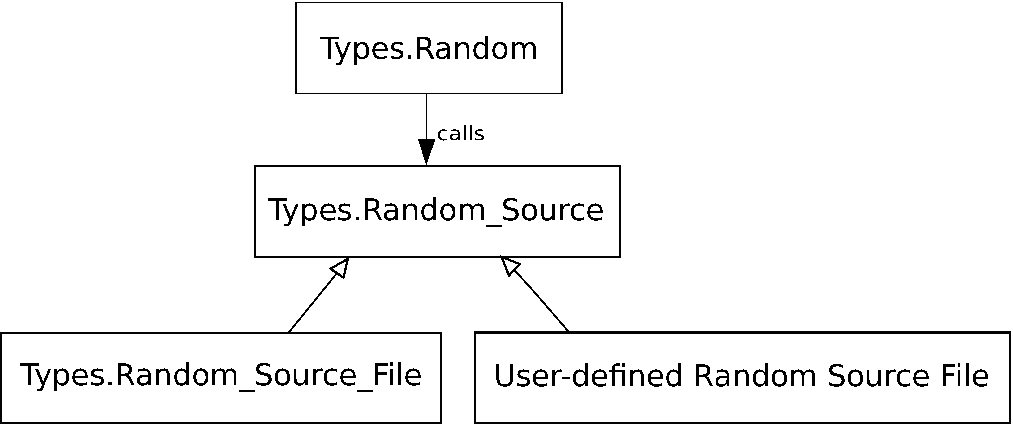
\includegraphics[scale=0.6]{./images/Random}
  \caption{The relationship among the data.}\label{WorkflowRandom}
\end{figure}
In the file \texttt{Random\_Source} the following abstract types and
procedures must be implemented:

\begin{lstlisting}{}
 package Fin renames Ada.Finalization;
 type Random_Source is abstract new Fin.Controlled with null record;
 type Random_Source_Access is access Random_Source;
 procedure Initialize(This: in out Random_Source) is abstract;
 procedure Read(This: in Random_Source; B: out Byte) is abstract;
\end{lstlisting}
When overwritting \texttt{Initialize()} in the file
\texttt{Random\_Source\_File}, the source path and source file are set
to "/dev/random" or some other user-defined random source. By calling
the procedure \texttt{Read()}, random bits are generated according to
the required type. After the reading procedure is finished, the source
file will be checked if it is closed, if it is open, then, a reading
error is raised.

%%%%%%%%%%%%%%%%%%%%%%%%%%%%%%%%%%%%%%%%%%%%%%%%%%%%%%%%%%%%%%%%%%
\section{"/dev/random"}\label{DevRandom}
In Linux, \texttt{Types.Random\_Source.File} assigns
\texttt{/dev/random} as the source file address by default. The device
node \texttt{/dev/random} can be seen as a special file that serves as
a random number generator or as a pseudorandom number
generator. Environmental noise will be gathered from device drivers
and other sources into an entropy pool, and then random numbers are
created \cite{dev-random}. When required, the \texttt{/dev/random} device
returns only bytes within the estimated number of bits of noise in the
entropy pool \cite{dev-random}.

If your operating system doesn't support \texttt{/dev/random} device, you can
install EGD (Entropy Gathering Daemon) by Brian Warners at the website
\textit{http://www.lothar.com/tech/cr\-ypto/}, it is a user-space
implementation of Linux-Kernel-Device \texttt{/dev/random}.

As mentioned in Section \ref{BasicRandom} the private part includes a
''Path'' variable. This variable indicates the path to a file, a named
pipe or a device storing cryptographically secure random
bits. Moreover, you can even link the ACL to a cryptographically
secure pseudorandom bit source on non-POSIX (Portable Operating System
Interface X) compliant operating systems, such as Windows XP.

%%%%%%%%%%%%%%%%%%%%%%%%%%%%%%%%%%%%%%%%%%%%%%%%%%%%%%%%%%%%%%%%%%

\subsection*{Example}
\begin{lstlisting}{}
   ...
   use Crypto.Types.Random_Source.File;
   Dev_U_Rand : Random_Source_File;
 begin
   Dev_U_Rand.Initialize("/dev/urandom");
   Crypto.Types.Random.Set(Dev_U_Rand);
   ...
\end{lstlisting}

\chapter{Crypto.Types.Elliptic\_Curves}\label{ConceptofElliptic}
For a deeper understanding of the elliptic curves, we provide an
introduction to elliptic curves for convenience of readers before we
continue with the algorithms in Section \ref{EllipticRoot}.

%%%%%%%%%%%%%%%%%%%%%%%%%%%%%%%%%%%%%%%%%%%%%%%%%%%%%%%
%%%%%%%%%%%%%%%%%%%%%%%%%%%%%%%%%%%%%%%%%%%%%%%%%%%%%%%

\section{Mathematical Concept of Elliptic Curves}
\paragraph{Finite Field $F_p^1$.}
For a given prime p, is an algebraic system defined on the number set
$F=\{0,1,\cdots,p-1\}$ with two operations \cite{SimpleTutorial}:

\begin{itemize}
\item Addition: $\forall$ $a,b\in F_p^1$\,, $r\equiv a+b \mod p$\,,
\item Multiplication: $\forall$ $a,b\in F_p^1$\,, $r\equiv a\times b \mod p$\,.
\end{itemize}

\paragraph{Galois Field.} A Galois field ($GF(2^m)$) is a finit field
where each element can be  expressed as a polynomial with degree less than $m$ (
$\forall$ $a \in GF(2^m)$\,,\,$\exists$ $m$ numbers $a_i\in
\{0,1\}$\,,\,$a=a_{m-1}x^{m-1}+\cdots +a_1x+a_0=(a_{m-1}\cdots a_0)$),
and satisfying \cite{SimpleTutorial}:
\begin{itemize}
\item Addition: $\forall$ $a,b\in GF(2^m)$\,, $a+b=c=(c_{m-1}\cdots
  c_0)$\,,\, $c_i=a_i+b_i\mod 2$ = $a_i\oplus b_i$\,,
\item Multiplication: $\forall$ $a,b\in GF(2^m)$\,, $a\times b=c$,
  $c=(\sum_{j=0}^{m-1}a_jx^j)\times (\sum_{j=0}^{m-1}b_jx^j)\mod
  f(x)$, where $f(x)=x^m+\sum_{j=0}^{m-1}f_jx^j$ is an irreducible
  polynomial with degree $m$\,.
\end{itemize}

\paragraph{Characteristic.} of a field $F$, $char(F)$, is the smallest
positive integer of $F$ which satisfies: $\sum_{i=1}^{n}I=0$, where
$I$ is the identity of the field multiplication \cite{SimpleTutorial}.

An elliptic curve $E$ over a finite field $F$ is given by the
Weierstrass equation:
\begin{equation}
  E : y^2 + a_1xy + a_3y = x^3 + a_2x^2 + a_4x + a_6\,, \label{GenerForm}
\end{equation}
where $a_1,a_2,a_3,a_4,a_6$ are coefficients in $F$.

A point ”at infinity” is defined. The Equation \ref{GenerForm} shall
be simplified under assumption about the characteristic of $F$ mapping
$(x,y)$ to $(x',y')$ by invertible linear transformations
\cite{Cohen}. These transformations correspond to morphisms of the
affine part of $E$ to the affine part of another elliptic curve $E'$,
and since the infinite point keeps unchanged an isomorphism between
$E$ and $E'$ is achieved \cite{Cohen}. After all transformations are
done, we change the notation and denote the transformed curve by $E$
with coordinates $(x,y)$ again \cite{Cohen}.\\ Supposed the
characteristic of $F$ is odd. The following transformations are made:
\begin{equation*}
x\mapsto x'\quad\hbox{and}\quad y\mapsto y'= y + \frac{1}{2}(a_1x +a_3)\,,
\end{equation*}
The equation of $E$ is expressed in the coordinates $(x',y')$, then
change notation and write $x$ for $x'$ and $y$ for $y'$, we get:
\begin{equation*}
E:y^2 = x^3 + \frac{b_2}{4}x^2 + \frac{b_4}{2}x + \frac{b_6}{4}\,,
\end{equation*}
where $b_2={a_1}^2+4a_2$\,,\,$b_4=2a_4+a_1a_3$ and
$b_6={a_3}^2+4a_6$\,.\\ Additionally if the characteristic of $F$ is
prime to 6. There goes another transformation:
\begin{equation*}
x\mapsto x'=x+\frac{b_2}{12}\quad\hbox{and}\quad y\mapsto y'\,,
\end{equation*}
and it becomes:
\begin{equation*}
E:y^2 = x^3 - \frac{c_4}{48}x - \frac{c_6}{864}\,,
\end{equation*}
where $c_4$ and $c_6$ are expressed in terms of $b_2,b_4,b_6$ as
\begin{equation*}
c_4={b_2}^2-24b_4\quad\hbox{and}\quad c_6=-{b_2}^2+36b_2b_4-216b_6\,.
\end{equation*}
So if $char(F)$ is prime to 6, Equation (\ref{GenerForm}) can be given
by a short Weierstrass equation of the type:
\begin{equation}
E:y^2 = x^3 + Ax + B\,, \label{SimpleForm}
\end{equation}
where $A,B\in F$.  The discriminant of the curve (\ref{GenerForm}) is
equal to the polynomial discriminant of the curve (\ref{SimpleForm}):
\begin{equation}
\bigtriangleup_{E} = -16(4A^3 + 27B^2)\,.
\end{equation}
A curve is non-singular if and only if the discriminant is unequal to zero.\\ 
 absolute invariant ($j$-invariant) $j_E$ of $E$ is given by
\begin{equation}
j_E = 12^3\frac{-4A^3}{\bigtriangleup_E}\,.\label{Invariant}
\end{equation} \\
If $char(F)=2$ or $3$, $E$ is supersingular if and only if its
$j$-invariant (\ref{Invariant}) is zero \cite{Cohen}.\\ For
$char(F)=2$, in the case of $a_1=0$, Equation (\ref{GenerForm}) can be
transformed to
\begin{equation}\label{Simple2}
E': y^2+Cy=x^3+Ax+B\,,
\end{equation}
where $A,B,C\in K$.\\
While in the case of $a_1\neq 0$, Equation (\ref{GenerForm}) can be transformed to
\begin{equation}\label{Simple3}
E': y^2+xy=x^3+Ax^2+B\,,
\end{equation}
where $A,B\in K$.\\ \ \\ 

\textbf{Group Law on Elliptic Curve: Point Addition and Point
  Doubling} \cite{Cohen}\\ For points $P=(x_1,y_1)$ and $Q=(x_2,y_2)$
on a curve $E$ of the form in Equation \ref{GenerForm}, $P\oplus
Q=(x_3,y_3)$ and\\
\begin{tabular}{llc}
\midrule \quad\quad $-P$ & = & $(x_1,-y_1-a_1x_1-a_3)$,\\ \quad\quad
$P\oplus Q$ & = & \quad\quad$(\lambda^2+a_1\lambda-a_2-x_1-x_2,\quad\lambda(x_1-x_3)-y_1-a_1x_3-a_3)$,\\ \bottomrule
\end{tabular}\\
where
\begin{equation*}
      \lambda =
      \left\{
       \begin{array}{ll}
       \frac{y_2-y_1}{x_2-x_1}\qquad\qquad\quad\quad \hbox{if $P\neq\pm Q$ (point addition)} \\
       \frac{3x_1^2+2a_2x_1+a_4-a_1y_1}{2y_1+a_1x_1+a_3}\quad\hbox{if $P=Q$ (point doubling)}
       \end{array}
      \right.
\end{equation*}\\
$\lambda$ is the slope of the line through $P$ and $Q$ in the case of
point addition, or the slope of the tangent through $P$ in the case of
point doubling.
\begin{figure}[h]
  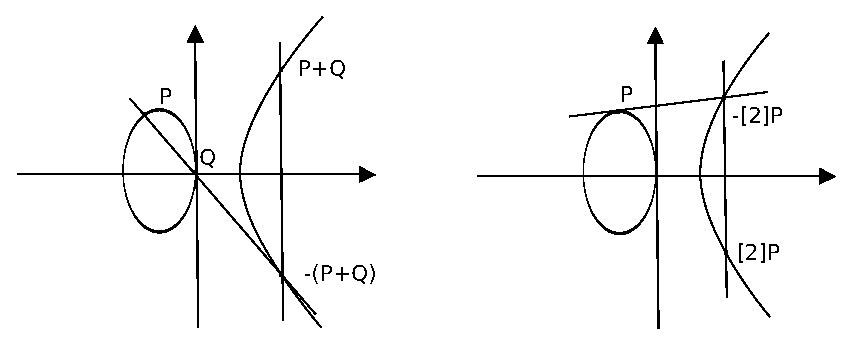
\includegraphics[scale=1]{./images/Group_law_of_ECC}
  \caption{The group law on elliptic curve. Adapted from \cite{Cohen}.}\label{EC}
\end{figure}

To illustrate the group law, $P$ and $Q$ are two points on the curve,
a third point can be made which is the intersection of the curve with
a line through $P$ and $Q$ (the left in Figure \ref{EC}). $P\oplus Q$
is given by mirroring the intersection point at the
$x$-axis. Furthermore, the sum of two points with the same
$x$-coordinate needs to be calculated (the right in Figure
\ref{EC}). A "point at infinity" $P_\infty$ is defined, it can be
understood as any line, which is parallel to the $y$-axis. This point
is the neutral point of the group, so that
$(x_1,y_1)\oplus(x_1,-y_1)=P_\infty$, i.e., $(x_1,-y_1)=-P$.

\hhline

In the ACL three types of elliptic curves are supported:
\begin{itemize}
\item $y^2 \equiv x^3 + Ax + B$ mod $p$ with $p \in \textbf{P} \setminus \{2,3\}$\\
      It is defined over the finite field $F_p$. (Section \ref{ZP})
\item $y^2 + xy \equiv x^3 + Ax^2 + B$ mod $f(z)$\\
      It is defined over the binary field $GF(2^{deg(f)})$. (Section \ref{NSS})\\
      \textbf{Precondition:} $f(z)$ is an irreducible polynomial.
\item $y^2 + Cy \equiv x^3 + Ax + B$ mod $f(z)$\\
      It defines supersingular elliptic curves over the binary field $GF(2^{deg(f)})$. (Section \ref{SS})\\
      \textbf{Precondition:} $f(z)$ is an irreducible polynomial.
\end{itemize}

%%%%%%%%%%%%%%%%%%%%%%%%%%%%%%%%%%%%%%%%%%%%%%%%%%%%%%%%%%%%%%%%%%%%%%%%%%%
%%%%%%%%%%%%%%%%%%%%%%%%%%%%%%%%%%%%%%%%%%%%%%%%%%%%%%%%%%%%%%%%%%%%%%%%%%%

\section{Root Package: Crypto.Types.Elliptic\_Curves}\label{EllipticRoot}
It is the root package of the elliptic curves. A basic type \texttt{EC\_Point} is defined for all three elliptic curve types.
\subsubsection*{Generic Part}
\begin{lstlisting}{}
  generic
  	with package Big is new Crypto.Types.Big_Numbers(<>);
\end{lstlisting}
\subsubsection*{Types}
The global type \texttt{EC\_Point} is defined.
\begin{lstlisting}{}
   -- (x,y)
  type EC_Point is record
  	 X : Big.Big_Unsigned;
    Y : Big.Big_Unsigned;
  end record;
  EC_Point_Infinity : constant EC_Point;
\end{lstlisting}
The constant \texttt{EC\_Point\_Infinity} of type \texttt{EC\_Point}
equals $\infty$. This point is located on each elliptic curve and
corresponds to the neutral element of addition.

%%%%%%%%%%%%%%%%%%%%%%%%%%%%%%%%%%%%%%%%%%%%%%%%%%%%%%%%%%%%%%%%

\subsubsection*{Procedures}
\begin{lstlisting}{}
  procedure Put(Item: in EC_Point, Base: in Number_Base := 10);
  procedure Put_Line( Item : in EC_Point, 
                      Base : in Number_Base := 10);
\end{lstlisting}
These two procedures output a \texttt{EC\_Point} in the standard output form of a tupel.\\

\noindent\textbf{Example:}
\begin{lstlisting}{}
  procedure Example_EC is
    P: EC_Point(X => Big_Unsigned_Three, Y => Big_Unsigned_One);
  begin
    Put(P);             -- Output: "(3,1)"
    Put(P, Base => 2);  -- Output: "(2#11#, 2#1#)"
  end Example_EC;
\end{lstlisting}

%%%%%%%%%%%%%%%%%%%%%%%%%%%%%%%%%%%%%%%%%%%%%%%%%%%%%%%%%%%%%%%%
%%%%%%%%%%%%%%%%%%%%%%%%%%%%%%%%%%%%%%%%%%%%%%%%%%%%%%%%%%%%%%%%

\section{Child Packages}
There are three child packages of the \texttt{Crypto.Types.Elliptic\_Curves}:
\begin{itemize}
\item \texttt{Crypto.Types.Elliptic\_Curves.Zp} \\
      -- elliptic curves over finite fields
\item \texttt{Crypto.Types.Elliptic\_Curves.NSS\_BF}\\
      -- non-supersingular elliptic curves over binary fields
\item \texttt{Crypto.Types.Elliptic\_Curves.SS\_BF}\\
      -- supersingular elliptic curves over binary fields
\end{itemize}
%implement each elliptic curves introduced above.
\subsection{Elliptic\_Curves.Zp}\label{ZP}
It implements an elliptic curve over a finite field $Z_p$.
\subsubsection*{Types}
In the package a variable type \texttt{Elliptic\_Curve\_Zp} is defined. It is only used in domain of this package.
\begin{lstlisting}{}
  --(A,B,P)
  type Elliptic_Curve_Zp is record
	 A : Big_Unsigned;
	 B : Big_Unsigned;
	 P : Big_Unsigned;
  end record;
\end{lstlisting}
$A,B,P$ are coefficients according to $y^2 \equiv x^3 + Ax + B$ mod $p$.
\subsubsection*{API}
\begin{lstlisting}{}
  procedure Init(A, B, P : in Big_Unsigned);
  procedure Init(ECZ     : in Elliptic_Curve_Zp);
  procedure Init(Len     : in Positive);
\end{lstlisting}
These are three ways to initialize the elliptic curves.  $A,B,P$ are
three compositions of the type \texttt{Elliptic\_Curve\_Zp}. The first
two procedures assign the parameters with delivered values. In the
third procedure, it searches prime numbers within the delivered bit
length and then initialises all variables.

These procedures make just an assignment or an initialization. Whether
the curve is an elliptic curve or not, can be tested by other
functions within the package.\\ 

\noindent\textbf{Exception:} If the
\texttt{Len} $<$ 3:\quad\texttt{Constraint\_Error}.

\hhline
\begin{lstlisting}{}
  function Is_Elliptic_Curve return Boolean;
\end{lstlisting}
This function tests whether the curve is an elliptic curve or not.
$P$ must be a prime number bigger than 3, and the discriminant of the
curve: $\bigtriangleup = -16(4a^3+27b^2)$ must be nonzero. It returns
true, if the curve meets the two requirements. When it fails, the
remaining functions may not return the desired results.

\hhline

\begin{lstlisting}{}
  function On_Elliptic_Curve(X : EC_Point) return Boolean;
\end{lstlisting}
This function tests, whether a point $X$ is on the elliptic curve or
not. In the situation that $X$ equals \texttt{EC\_Point\_Infinity},
the function returns true.

\hhline

\begin{lstlisting}{}
  function Negative   (X : EC_Point)           return EC_Point;
  function Is_Negative(X : EC_Point)           return Boolean;
  function Is_Negative(Left, Right : EC_Point) return Boolean;
\end{lstlisting}
The function \texttt{Negative()} returns the value $-X$.\\ The
function \texttt{Is\_Negative()} with parameter $X$ tests if $X$
equals \texttt{EC\_Point\_Infinity} or if $-X$ equals
\texttt{Big\_Unsigned\_Zero}. It returns true if one of the two
situations happens.\\ The last function test if both \texttt{Left} and
\texttt{Right} equal \texttt{EC\_Point\_Infinity}, or whether
\texttt{Left} is the negative of \texttt{Right}.

\hhline

\begin{lstlisting}{}
  function "+"(Left, Right : EC_Point) return EC_Point;
  function "-"(Left, Right : EC_Point) return EC_Point;
  function "*"(Left  : Big_Unsigned; Right : EC_Point) return EC_Point;
\end{lstlisting}
Here the basic operations for variables of \texttt{EC\_Point} are defined.

\hhline

\begin{lstlisting}{}
  function Double(X : EC_Point) return EC_Point;
\end{lstlisting}
This function calculates $2X$.\\

%%%%%%%%%%%%%%%%%%%%%%%%%%%%%%%%%%%%%%%%%%%%%%%%%%%%%%%%%%%%%%%%%

\subsection{Elliptic\_Curves.NSS\_BF}\label{NSS}
In this package the elliptic curve $y^2 + xy \equiv x^3 + Ax^2 + B$
mod $f(z)$ is implemented. Some commen operations have been already
introduced in \texttt{Crypto.Types.Elliptic\_Curves.Zp}, Section
\ref{ZP} can be refered for details.
\subsubsection*{API}
\begin{lstlisting}{}
  procedure Init(A, B, F : in Big_Unsigned);
\end{lstlisting}
The procedure makes the initialization. $A,B$ are two coefficients,
and $F$ is a polynomial that creates the binary field
$GF(2^{deg(F)})$.

\hhline

\begin{lstlisting}{}
  function Is_Elliptic_Curve return Boolean;
\end{lstlisting}
The funtion tests if the curve after the initialization is a valid
elliptic curve or not. It tests if F is irreducibel, and computes if
the discriminant of the elliptic curve is nonzero. Unfortunately the
test of $F$ is still in plan.\\
\subsection{Elliptic\_Curves.SS\_BF}\label{SS}
This package implements the elliptic curve $y^2 + Cy = x^3 + Ax + B$
mod $f(z)$. Some commen operations have been already introduced in
\texttt{Crypto.Types.Elliptic\_Curves.Zp}, Section \ref{ZP} can be
refered for details.
\subsubsection*{API}
\begin{lstlisting}{}
  procedure Init(A, B, C, F : in Big_Unsigned);
\end{lstlisting}
$A,B,C$ are the coefficients of the curve, and $F$ is a polynomial
that creates the binary field $GF(2^{deg(F)})$.

\hhline

\begin{lstlisting}{}
  function Is_Elliptic_Curve return Boolean;
\end{lstlisting}
It tests if the curve after the initialization is a valid elliptic
curve or not. It tests if F is irreducibel, and computes if the
discriminant of the elliptic curve is nonzero. Unfortunately the test
of $F$ is still in plan.\\
\subsection{Elliptic Curves Database $Z_p$}
One elliptic curves database of this form
\begin{itemize}
\item $y^2 = x^3 + Ax + B$ mod $p$ with $p \in \textbf{P} \setminus \{2,3\}$ \\
      -- elliptic curve defined over the finite field $Z_p$.
\end{itemize}
is provided in the ACL, which contains the elliptic curves published
by NIST (National Institute of Standards and Technology). The
following curves are included: 
\begin{center}
Curve P-192/244/384/521 and Test Curve (5-bit).
\end{center}


\subsubsection*{Generic Part}
\begin{lstlisting}{}
  package Elliptic_Curve_Database_Map is
      new Ada.Containers.Ordered_Maps (Key_Type => Bit_Length,
                   Element_Type => Precomputed_Elliptic_Curve);
\end{lstlisting}
\subsubsection*{Types}
This package defines two types: \texttt{Bit\_Length} and \texttt{Precomputed\_Elliptic\_Curve}.
\begin{lstlisting}{}
  type Bit_Length is new natural;
  type Precomputed_Elliptic_Curve is record
    P : String(1..192) := (others=>' ');   -- prime modulus
    R : String(1..192) := (others=>' ');   -- order
    S : String(1..192) := (others=>' ');   -- 160-bit input seed to SHA-1
    C : String(1..192) := (others=>' ');   -- output of SHA-1
    B : String(1..192) := (others=>' ');   -- coefficient b
    Gx : String(1..192) := (others=>' ');  -- base point x coordinate
    Gy : String(1..192) := (others=>' ');  -- base point y coordinate
    length : Bit_Length;	           -- bit length
  end record;
\end{lstlisting}
\subsubsection*{Procedures}
\begin{lstlisting}{}
  procedure Get_Elliptic_Curve(ECZ    : out Elliptic_Curve_Zp;
                               ECP    : out EC_Point;
                               order  : out Big_Unsigned;
                               length : in  Bit_Length);
\end{lstlisting}
This procedure takes related variables from the database, which are
required to compute an elliptic curve. The curve has at least a
cryptographic security in \texttt{length}. \\

\noindent\textbf{Exception:} The
\texttt{length} has a range from 0 to 521 bits (max. bit length = 521
bits). If a \texttt{length} value is not
included:\quad\texttt{LEN\_ERROR}.\\

\noindent\textbf{Example:}
\begin{lstlisting}{}
  with Crypto.Types; use Crypto.Types;
  with Crypto.Types.Big_Numbers;
  with Crypto.Types.Elliptic_Curves.Zp;
  with Crypto.Types.Elliptic_Curves.Zp.Database;

  procedure Example_EC_DB_ZP is
    package Big is new Crypto.Types.Big_Numbers(Size);
    use Big;
    package EC is new Crypto.Types.Elliptic_Curves(Big);
    use EC;
    package Zp is new EC.Zp;
    use Zp;
    package DB is new Zp.Database;
    use DB;
    EC_ZP : Elliptic_Curve_Zp;
    EC_P  : EC_Point;
    order : Big_Unsigned;
  begin
    Get_Elliptic_Curve(EC_ZP, EC_P, order, 168);
  end Example_EC_DB_ZP;
\end{lstlisting}

\chapter{Crypto.Types.Big\_Numbers}
The package provides a generic type \texttt{Big\_Unsigned} with a set
of procedures and functions. This type uses internally an array, which
consists of 32-bit words. And this array is as a modular type
interpreted. For this reason, it is only possible to generate
variables of type \texttt{Big\_Unsigned} with that, their bit length
is a multiple of 32 bits. Since the package works without pointer and
inline assembler, it is much slower than e.g. for efficiency optimized
MPI (multi-precision-integers) of
GnuPG\footnote{http://www.gnupg.org/documentation/manuals/gcrypt/MPI-library.html,
  November 2012}. This big number package is originally based on the
Big Number library\footnote{http://bignumber.chez.com/, November 2012}
by Jerome Delcourt, which should be used here. But it turned out that
the library didn't meet some desired requirements. So this package
would be completely rewritten. A significant contribution to the
current code is the analysis of the source code from
\texttt{java.math.BigInteger}
\footnote{http://docs.oracle.com/javase/1.4.2/docs/api/java/math/BigInteger.html,
  November 2012} and
BeeCrypt\footnote{http://sourceforge.net/projects/beecrypt/, November
  2012} library by Bob Deblier.% and also the following codes.  The
package is specified in Crypto.Types.Big\_Numbers.

\section{API}
\subsubsection*{Generic Part}
\begin{lstlisting}{}
  generic
    Size : Positive;
\end{lstlisting}
\paragraph{Exception:} If Size $\not= k \cdot 32,\; k \in N$:\quad
\texttt{Constraint\_Size\_Error}.
\newpage

\subsubsection*{Types}
\begin{lstlisting}{}
  type Big_Unsigned is private;
\end{lstlisting}
It is the basic type in the package. \texttt{Big\_Unsigned} represents
a modular number of n ($n = k \cdot 32$) bits. A variable of this type
will be always initialized with a constant named
\texttt{Big\_Unsigned\_Zero}.

\hhline
\begin{lstlisting}{}
  subtype Number_Base is Integer range 2 .. 16;
\end{lstlisting}
The type will be needed later for the conversion from a
\texttt{Big\_Unsigned} to a string. A \texttt{Big\_Unsigned} variable
can be represented as a number based on a base from this
subtype.

\hhline
\subsubsection*{Constants}
\begin{lstlisting}{}
  Big_Unsigned_Zero   : constant Big_Unsigned; -- 0
  Big_Unsigned_One    : constant Big_Unsigned; -- 1
  Big_Unsigned_Two    : constant Big_Unsigned; -- 2
  Big_Unsigned_Three  : constant Big_Unsigned; -- 3
  Big_Unsigned_Four   : constant Big_Unsigned; -- 4
  Big_Unsigned_Ten    : constant Big_Unsigned; -- 10
  Big_Unsigned_Sixteen: constant Big_Unsigned; -- 16
  Big_Unsigned_First  : constant Big_Unsigned; -- 0
  Big_Unsigned_Last   : constant Big_Unsigned; -- "Big_Unsigned'Last"
\end{lstlisting}

%%%%%%%%%%%%%%%%%%%%%%%%%%%%%%%%%%%%%%%%%%%%%%%%%%%%%%%%%%%%%%%%%
%%%%%%%%%%%%%%%%%%%%%%%%%%%%%%%%%%%%%%%%%%%%%%%%%%%%%%%%%%%%%%%%%
\subsubsection*{Comparison Operations}
\begin{itemize}
\item Between two values of the same type \texttt{Big\_Unsigned}:
\end{itemize}
\begin{lstlisting}{}
  function "=" (Left, Right : Big_Unsigned) return Boolean;
  function "<" (Left, Right : Big_Unsigned) return Boolean;
  function ">" (Left, Right : Big_Unsigned) return Boolean;
  function "<="(Left, Right : Big_Unsigned) return Boolean;
  function ">="(Left, Right : Big_Unsigned) return Boolean;

  function Min(X, Y : in Big_Unsigned) return Big_Unsigned;
  function Max(X, Y : in Big_Unsigned) return Big_Unsigned;
\end{lstlisting}
\begin{itemize}
\item Between one value of type \texttt{Big\_Unsigned} and one value
  of type \texttt{Mod\_Type}, also vice versa.
\end{itemize}
\begin{lstlisting}{}
  function "="(Left : Big_Unsigned; Right : Mod_Type) return Boolean;
  function "<"(Left : Big_Unsigned; Right : Mod_Type) return Boolean;
  function ">"(Left : Big_Unsigned; Right : Mod_Type) return Boolean;
  function "<="(Left: Big_Unsigned; Right : Mod_Type) return Boolean;
  function ">="(Left: Big_Unsigned; Right : Mod_Type) return Boolean;
\end{lstlisting}
\subsubsection*{Basic Operations}
The basic functions can be used to operate values of
\texttt{Big\_Unsigned} and \texttt{Mod\_Type}. Additionally, the
functions $"+","-","*","/"$ can be applied on two values, which are
both of type \texttt{Big\_Unsigned}.

\begin{lstlisting}{}
  function "+"(Left:Big_Unsigned;Right:Mod_Type) return Big_Unsigned;
  function "-"(Left:Mod_Type;Right:Big_Unsigned) return Big_Unsigned;
  function "*"(Left:Big_Unsigned;Right:Mod_Type) return Big_Unsigned;
  function "/"(Left:Mod_Type;Right:Big_Unsigned) return Big_Unsigned;

  function "xor"(Left, Right : Big_Unsigned) return Big_Unsigned;
  function "or" (Left, Right : Big_Unsigned) return Big_Unsigned;
  function "and"(Left, Right : Big_Unsigned) return Big_Unsigned;
  function "and"(Left  : Big_Unsigned;
  					  Right : Mod_Type) return Big_Unsigned;
  function "and"(Left  : Mod_Type;
  					  Right : Big_Unsigned) return Big_Unsigned;
  function "**" (Left, Right : Big_Unsigned) return Big_Unsigned;
  function "mod"(Left, Right : Big_Unsigned) return Big_Unsigned;
  function "mod"(Left  : Big_Unsigned;
  					  Right : Mod_Type) return Big_Unsigned;
\end{lstlisting}

%%%%%%%%%%%%%%%%%%%%%%%%%%%%%%%%%%%%%%%%%%%%%%%%%%%%%%%%%%%%%%%%%%

\subsubsection*{Multiplication}
In addition to the elementary multiplication functions, further
multiplication algorithms are implemented to develop their potentials
in \texttt{Big\_Unsigned}.\\

\begin{lstlisting}{}
  function Russ(Left, Right: Big_Unsigned) return Big_Unsigned;
\end{lstlisting}
The Russian multiplication is a systematic method, which does not
require the multiplication table, only the ability to multiply and
divide by 2, and to add, details can be found in \cite{Russ}.

\hhline

\begin{lstlisting}{}
  function Karatsuba(Left, Right : Big_Unsigned) return Big_Unsigned;
  function Karatsuba_P(Left,Right: Big_Unsigned) return Big_Unsigned;
\end{lstlisting}
The Karatsuba algorithm can reduce the multiplication of two n-digit
numbers to at most $3 n^{\log_2 3}\approx 3 n^{1.585}$ single-digit
multiplications usually (and exactly $n^{\log_2 3}$ when n is a power
of 2) \cite{DBLP:reference/crypt/2011}. In parallel Karatsuba
function, the product is calculated in tasks.

\hhline
\begin{lstlisting}{}
  function Toom_Cook(Left, Right : Big_Unsigned) return Big_Unsigned;
  function Toom_Cook_P(Left,Right: Big_Unsigned) return Big_Unsigned;
\end{lstlisting}
The Toom-Cook multiplication splits up two large integers $a$ and $b$
into $k$ smaller parts (each of length $l$ ), and performs operations
on the parts. As $k$ grows, the multiplication sub-operations may be
combined, thus the overall complexity can be reduced, and the
multiplication sub-operations can be computed recursively using
Toom-Cook multiplication again, and so on
\cite{DBLP:reference/crypt/2011}.

\paragraph{Remarks.} All algorithms can be called explicitly and used
for multiplication of two \texttt{Big\_Unsigned} values.  A
performance improvement can then be achieved by combining different
algorithms, which contain different strengths. In the ACL, by calling
the elementary multiplication (function $'*'$) the sum of two
parameters' bit length is compared to the length of
\texttt{Mod\_Type}. The elementary multiplication is used for small
factors, for large bit length (between 2800 bits and 3600 bits) the
parallel Karatsuba (function \texttt{Karatsuba\_P()}) will be called,
and for the length, which is longer than 3600 bits, the parallel
Toom\_Cook algorithm (function \texttt{Toom\_Cook\_P()}) will come in
use.
%%%%%%%%%%%%%%%%%%%%%%%%%%%%%%%%%%%%%%%%%%%%%%%%%%%%%%%%%%%%%%%%%
%%%%%%%%%%%%%%%%%%%%%%%%%%%%%%%%%%%%%%%%%%%%%%%%%%%%%%%%%%%%%%%%%
\section{Utils}
\texttt{Crypto.Types.Big\_Numbers.Utils} is a separate body of
\texttt{Crypto.Types.Big\_Numbers}. Many useful functions and
procedures are provided.
\begin{lstlisting}{}
  procedure Swap(X, Y : in out Big_Unsigned);
\end{lstlisting}
The two parameters are exchanged.

\hhline
\begin{lstlisting}{}
  procedure Set_Least_Significant_Bit(X : in out Big_Unsigned);
  procedure Set_Most_Significant_Bit (X : in out Big_Unsigned);
\end{lstlisting}
The first procedure sets the least significant (the most right) bit of
X to 1. Then, X is after calling this procedure always odd. The second
procedure sets the most significant (the most left) bit of X to
1. This procedure ensures that X has always n bits.

\hhline
\begin{lstlisting}{}
  function Is_Odd (X : Big_Unsigned) return Boolean;
  function Is_Even(X : Big_Unsigned) return Boolean;
\end{lstlisting}
The function \texttt{Is\_Odd()} returns true if X is odd, and the
function \texttt{Is\_Even()} returns true if X is even.

\hhline
\begin{lstlisting}{}
  procedure Inc(X : in out Big_Unsigned);
  procedure Dec(X : in out Big_Unsigned);
\end{lstlisting}
The procedure \texttt{Inc()} increases X by 1, and the procedure
\texttt{Dec()} decreases X by 1.x

\hhline
\begin{lstlisting}{}
  function Shift_Left (Value  : Big_Unsigned;
                       Amount : Natural) return Big_Unsigned;

  function Shift_Right(Value  : Big_Unsigned;
                       Amount : Natural) return Big_Unsigned;
\end{lstlisting}
The function \texttt{Shift\_Left()} calculates
$Value\,*\,2^{Amount}$. And the function \texttt{Shift\_Right()}
calculates $\lfloor Value\, /\,
2^{Amount}\rfloor$.\\

\noindent\textbf{Example:}
\begin{lstlisting}{}
    X : Big_Unsigned := 2#101011#;
  begin
    X := Shift_Right(X, 2);  -- X := 2#001010#
  end;
\end{lstlisting}
X is originally assigned by $2\#101011\#$, decimally equals 43. After
calling the function \texttt{Shift\_Right()}, X is shifted to right
for 2 positions and becomes $2\#001010\#$, decimally equals $\lfloor
43\,/\,2^2 \rfloor$ = 10.

\hhline
\begin{lstlisting}{}
  function Rotate_Left (Value  : Big_Unsigned;
  							   Amount : Natural) return Big_Unsigned;
  function Rotate_Right(Value  : Big_Unsigned; 
  							   Amount : Natural) return Big_Unsigned;
\end{lstlisting}
The function \texttt{Rotate\_Left()} makes rotation of a value to the
left. It mathematically calculates $((Value * 2^{Amount})\; \oplus\;
(\lfloor Value\, /\, 2^{Size - Amount}\rfloor))$ $\bmod\; 2^{Size}$.
The parameter \texttt{Amount} will be calculated through:

\begin{lstlisting}{}
  L : constant Natural := Amount mod Size;
\end{lstlisting}
then, rotation is made by combining function \texttt{Shift\_Left()}
and \texttt{Shift\_Right()}:

\begin{lstlisting}{}
  return Shift_Left(Value,L) xor Shift_Right(Value, Size-L);
\end{lstlisting}
The function \texttt{Rotate\_Right()} makes rotation of a value to the
right. It mathematically calculates $((Value * 2^{Size - Amount})\;
\oplus\; (\lfloor Value / 2^{Amount}\rfloor))$ $\bmod\; 2^{Size}$, as
shown in the following:
\begin{lstlisting}{}
  R : constant Natural := Amount mod Size;
  return Shift_Right(Value,R) xor Shift_Left(Value, Size-R);
\end{lstlisting}

\hhline
\begin{lstlisting}{}
  function Get_Random return Big_Unsigned;
\end{lstlisting}
This function generates a random number in the interval [
  $0\ldots$\texttt{Big\_Unsigned\_Last} ].

\hhline
\begin{lstlisting}{}
  function Lowest_Set_Bit(X : Big_Unsigned) return Natural;
\end{lstlisting}
This function returns the position of the least significant bit in X,
which has the value "1".\\

\noindent\textbf{Exception:} If X = 0
(\texttt{Big\_Unsigned\_Zero}):\quad \texttt{Is\_Zero\_Error}.

\hhline
\begin{lstlisting}{}
  function Gcd(Left, Right : Big_Unsigned) return Big_Unsigned;
\end{lstlisting}
The function calculates the greatest common divisor of the two values.\\

\hhline
\begin{lstlisting}{}
  function Length_In_Bytes(X : Big_Unsigned) return Natural;
  function Bit_Length     (X : Big_Unsigned) return Natural;
\end{lstlisting}
The function \texttt{Length\_In\_Bytes()} calculates the number of
bytes which are required to output X as a byte array. The function
\texttt{Bit\_Length()} returns the bit length of X.

\hhline
\begin{lstlisting}{}
  function To_Big_Unsigned(X : Bytes)        return Big_Unsigned;
  function To_Bytes       (X : Big_Unsigned) return Bytes;
\end{lstlisting}
The two functions provide conversion between values of
\texttt{Big\_Unsigned} and bytes.  The function
\texttt{To\_Big\_Unsigned()} converts X of bytes to a
\texttt{Big\_Unsigned} value B. The function \texttt{To\_Bytes()}
converts a variable X of the type \texttt{Big\_Unsigned} to a byte
array B.\\

\noindent\textbf{Exception:} If the bit length of X is greater than
\texttt{Size}:\quad \texttt{Constraint\_Error}.

\hhline
\begin{lstlisting}{}
  function To_Mod_Types   (X : Big_Unsigned) return Mod_Types;
  function To_Big_Unsigned(X : Mod_Types)    return Big_Unsigned;
\end{lstlisting}
The two functions make conversion between values of
\texttt{Mod\_Types} and \texttt{Big\_Unsigned}.\\

\noindent\textbf{Exception:}
In the function \texttt{To\_Big\_Unsigned()}, if
the bit length of X is greater than \texttt{Size}:\quad
\texttt{Constraint\_Error}.

\hhline
\begin{lstlisting}{}
  function To_String(Item : Big_Unsigned;
                     Base : Number_Base := 10) return String;
  function To_Big_Unsigned(S : String)         return Big_Unsigned;
\end{lstlisting}
The function \texttt{To\_String()} converts \texttt{Item} to a
string. The conversion can be done with a Base (Base $\in \{2,\ldots
,16\}$). The output string has the following structures:
\begin{itemize}
\item \textbf{Base  = 10: } a number with the base 10 (e.g.''1325553'')
\item \textbf{Base /= 10: } a number with the base B\# (e.g.''12\#AB45623A3402\#'')
\end{itemize}
The function \texttt{To\_Big\_Unsigned()} makes transformation of a
string S to a \texttt{Big\_Unsigned} value. The string will be
displayed as a number of decimal notation or with a base (Base $\in
\{2,\ldots ,16\})$ and should have the following structures:
\begin{itemize}
\item a number with base B\# (e.g.''16\#FF340A12B1\#'')
\item a number with base 10 (e.g.''333665'')
\end{itemize}

\noindent\textbf{Exceptions:}
\begin{itemize}
\item If S is a null string:\quad \texttt{Conversion\_Error}.
\item If S has an invalid base:\quad \texttt{Conversion\_Error}.
\item If S has invalid characters:\quad \texttt{Conversion\_Error}.
\end{itemize}

\hhline
\begin{lstlisting}{}
  procedure Put(Item : in Big_Unsigned;
                Base : in Number_Base := 10);

  procedure Put_Line(Item : in Big_Unsigned;
                     Base : in Number_Base := 10);
\end{lstlisting}
The procedure \texttt{Put()} outputs the \texttt{Big\_Unsigned}
variable in standard format with a Base (Base $\in \{2,\ldots
,16\})$. The procedure \texttt{Put\_Line()} outputs the value in
standard format including a line break.

\hhline
\begin{lstlisting}{}
  procedure Big_Div(Dividend, Divisor   : in  Big_Unsigned;
                    Quotient, Remainder : out Big_Unsigned);

  procedure Short_Div(Dividend  : in  Big_Unsigned;
                      Divisor   : in  Mod_Type;
                      Quotient  : out Big_Unsigned;
                      Remainder : out Mod_Type);
\end{lstlisting}
The procedure \texttt{Big\_Div()} calculates the quotient
(\texttt{Quotient}) and the rest (\texttt{Remainder}) of two
\texttt{Big\_Unsigned} variables, meanwhile the procedure
\texttt{Short\_Div()} makes the same calculation between a
\texttt{Big\_Unsigned} variable and a \texttt{Mod\_Type} variable. The
following rules are applied:
\begin{itemize}
\item Quotient := $\lfloor \frac{Dividend}{Divisor} \rfloor$
\item Remainder :=  $Dividend\; \bmod\; Divisor$
\end{itemize}
\textbf{Exception:} If $Divisor$ = 0:\quad \texttt{Division\_By\_Zero}.

%%%%%%%%%%%%%%%%%%%%%%%%%%%%%%%%%%%%%%%%%%%%%%%%%%%%%%%%%%%%%%%%%%%%
%%%%%%%%%%%%%%%%%%%%%%%%%%%%%%%%%%%%%%%%%%%%%%%%%%%%%%%%%%%%%%%%%%%%


\section{Mod\_Utils}
The \texttt{Crypto.Types.Big\_Numbers.Mod\_Utils} is another separate
body of \texttt{Crypto.Types.\-Big\_Numbers}. Functions and
procedures, which are needed for Public-Key-Cryptography, will be
introduced. All the operations in this package are mod N.
\begin{lstlisting}{}
  function Add (Left, Right, N : Big_Unsigned) return Big_Unsigned;
  function Sub (Left, Right, N : Big_Unsigned) return Big_Unsigned;
  function Div (Left, Right, N : Big_Unsigned) return Big_Unsigned;
  function Mult(Left, Right, N : Big_Unsigned) return Big_Unsigned;
\end{lstlisting}
These are the four basic functions for two values, the result should be mod N.\\

\noindent\textbf{Exception in \texttt{Div()}:} If Right = 0
(\texttt{Big\_Unsigned\_Zero}): \texttt{Division\_By\_Zero}.


\hhline
\begin{lstlisting}{}
  function Pow(Base, Exponent, N : Big_Unsigned) return Big_Unsigned;
\end{lstlisting}
It calculates $Base^{Exponent}$ (mod N).

\hhline
\begin{lstlisting}{}
  function Get_Random (N : Big_Unsigned) return Big_Unsigned;
\end{lstlisting}
It returns a random \texttt{Big\_Unsigned} variable (mod N).

\hhline
\begin{lstlisting}{}
  function Inverse (X,N: Big_Unsigned) return Big_Unsigned;
\end{lstlisting}
It returns the inverse (with respect of multiplication) of X (mod
N). If no inverse of X exists, \texttt{Big\_Unsigned\_Zero} will be
returned.

\hhline
\begin{lstlisting}{}
  function Get_Prime  (N : Big_Unsigned) return Big_Unsigned;
  function Get_N_Bit_Prime(N : Positive) return Big_Unsigned;
\end{lstlisting}
The function \texttt{Get\_Prime()} calculates with an overwhelming
probability a prime variable P (mod N), while the function
\texttt{Get\_N\_Bit\_Prime()} calculates a N-bit prime result.\\

\noindent\textbf{Exception:}
\begin{itemize}
\item In the function \texttt{Get\_Prime()}, if N $<=$ 2:\quad\texttt{Constraint\_Error}.
\item In the function \texttt{Get\_N\_Bit\_Prime()}, if N = 1 or\; N $>$ \texttt{Size}:\quad\texttt{Constraint\_Error}.
\end{itemize}

\hhline
\begin{lstlisting}{}
  function Is_Prime(X : Big_Unsigned) return Boolean;
\end{lstlisting}
This function returns true if X is prime or false if X is not prime
with an overwhelming probability. An internal function
\texttt{Pass\_Prime\_Test()} is called to check X.\\

\paragraph{How it  works.}
\begin{enumerate}
\item Test if a one digit prime (2,3,5,7) divides $X$.
\item Test if a two digit prime number divides $X$.
\item Test if a three digit prime number divides $X$.
\item Test if X is a "Lucas-Lehmer" prime\footnote{http://en.wikipedia.org/wiki/Lucas-Lehmer\_primality\_test, November 2012.}.
\item Compute N random \texttt{Big\_Unsigned} values and test if one
  of those is an Miller-Rabin
  wittness\footnote{http://en.wikipedia.org/wiki/Miller-Rabin\_primality\_test,
    November 2012.} ($\,1<N<51$, where N depends on the bit length of X).
\end{enumerate}

\hhline
\begin{lstlisting}{}
  function Looks_Like_A_Prime(X : Big_Unsigned) return Boolean;
\end{lstlisting}
It's a weaker but faster prime test than function
\texttt{Is\_Prime()}. It returns false with high probability if $X$ is
not prime. An internal function \texttt{Pass\_Prime\_Test()} is called
to check X.

\paragraph{How it works.} This function acts much the same as the
function \texttt{Is\_Prime()}, with the difference that the
Miller-Rabin-Test is replaced by a simpler but unreliable prime number
test, which runs 2-50 times to generate random numbers and test if it
is a divisor of X (while Miller-Rabin-Test tests if it is a
Miller-Rabin wittness). When the divisor of X doesn't exist, the
function returns true.

\hhline
\begin{lstlisting}{}
  function Passed_Miller_Rabin_Test(X : Big_Unsigned;
                                   S : Positive) return Boolean;
\end{lstlisting}
It returns true only when X passes a certain number of Miller-Rabin
tests (S iterations). The probability that a pseudo prime number
passes this test is smaller than $\frac{1}{2^{2S}}$.

\hhline
\begin{lstlisting}{}
  function Jacobi(X, N : Big_Unsigned) return Integer;
\end{lstlisting}
This function computes the Jacobi-symbol of X from $Z_N$.\\

\noindent\textbf{Precondition:} N must be odd.\\

\noindent\textbf{Returned values:} \\
\begin{tabular}{p{\textwidth}}
\quad 0 : if X mod N = 0\\
\quad 1 : if X is a quadratic resuide mod N (for some integer b, $X=b^2$ mod N)\\
\quad -1 : if X is a quadratic non-resuide mod N (there is no such b)
\end{tabular}\ \\

\noindent\textbf{Exception:} If X is even:\quad \texttt{Constraint\_Error}.


%%%%%%%%%%%%%%%%%%%%%%%%%%%%%%%%%%%%%%%%%%%%%%%%%%%%%%%%%%%%%%%%
%%%%%%%%%%%%%%%%%%%%%%%%%%%%%%%%%%%%%%%%%%%%%%%%%%%%%%%%%%%%%%%%
\section{Binfield\_Utils}
It's also a separate body of
\texttt{Crypto.Types.Big\_Numbers}. Functions and procedures in this
package receive variables of type \texttt{Big\_Unsigned} from the
field $GF(2^m)$ as parameters. This package is specified in
\texttt{Crypto.Types.Big\_Numbers.Binfield\_Utils}.\\

\noindent\textbf{Example:}
\begin{lstlisting}{}
  -- The 1st, 2nd and 6th bit of A are to be set.
  -- After calculation A is equal to z^5 + z + 1
  A := Big_Unsigned_One;
  A := A xor Shift_left(Big_Unsigned_One,1);
  A := A xor Shift_left(Big_Unsigned_One,5);
\end{lstlisting}
In the following functions, the variable F of type
\texttt{Big\_Unsigned} is an irreducible polynom f(z) of a degree
$m$.

\begin{lstlisting}{}
  function B_Add(Left, Right :Big_Unsigned) return Big_Unsigned;
  function B_Sub(Left, Right :Big_Unsigned) return Big_Unsigned;
\end{lstlisting}
The two functions calculate \texttt{Left} xor \texttt{Right}, which
corresponds to addition or subtraction in $GF(2^m)$.


\hhline
\begin{lstlisting}{}
  function B_Mult(Left, Right, F :Big_Unsigned) return Big_Unsigned;
  function B_Div (Left, Right, F :Big_Unsigned) return Big_Unsigned;
\end{lstlisting}
The function \texttt{B\_Mult()} computes $Left*Right$ mod F. In the
function \texttt{B\_Div()} it uses \texttt{B\_Mult()} with the inverse
of the value \texttt{Right}.

\hhline
\begin{lstlisting}{}
  function B_Square(A, F : Big_Unsigned) return Big_Unsigned;
\end{lstlisting}
It computes $A^2$ mod F.

\hhline
\begin{lstlisting}{}
  function B_Mod(Left, Right : Big_Unsigned) return Big_Unsigned;
\end{lstlisting}
It computes \texttt{Left} mod \texttt{Right}.

\hhline
\begin{lstlisting}{}
  function B_Inverse(X, F : Big_Unsigned) return Big_Unsigned;
\end{lstlisting}
It returns $X^{(-1)}$ mod F.

\chapter{Crypto.Types.Nonces}
This package provides a generic type \texttt{Nonce} with related
procedures and functions. "A nonce is a cryptographic input value
which must never repeat within a given context"
\cite{DBLP:conf/isw/Zenner09}. Nonces are important for the security
of many cryptographic building blocks, such as block ciphers, modes of
operations, as well as message authentication codes
\cite{DBLP:conf/isw/Zenner09}. For a message $M$ after encryption with
the same key but different nonce values $N_1\neq N_2$, we'll get with
great probability that $E_K(M,N_1)\neq E_K(M,N_2)$. The package is
specified in \texttt{Crypto.Types.Nonces}.


\section{Crypto.Types.Mutexes}
In order to avoid some confusions during the process of calculation by
different threads, a state value of type \texttt{Mutex\_Type}
(\texttt{Crypto.Types.Mutexes}) is used. We use this state value
combined with the data to indicate if the data is seized by some
thread. If yes, then the status is locked (owned is "true"), and the
other threads should wait until it's free. Mutex guarantees that only
one thread can process the resource at one time, and the other
threads, if more than one thread, should wait in a queue for the
resource. Another status is named released (owned is "false") if the
resource is hold by no thread (free state).

\begin{lstlisting}{}
  protected type Mutex_Type is
    entry Seize;
    procedure Release;
  private
    Owned : Boolean := False;
  end Mutex_Type;
\end{lstlisting}
This workflow is called rendezvous in Ada, in the above example they
interact indirectly through shared data. Rendezvous is similar to the
human situation when two people meet, they perform a transaction and
then go on independently \cite{Ada2005}.

%%%%%%%%%%%%%%%%%%%%%%%%%%%%%%%%%%%%%%%%%%%%%%%%%%%%%%%%%%%%%%%%%
%%%%%%%%%%%%%%%%%%%%%%%%%%%%%%%%%%%%%%%%%%%%%%%%%%%%%%%%%%%%%%%%%
\section{API}
\subsubsection*{Generic Part}
\begin{lstlisting}{}
  generic
    type Block is private;
\end{lstlisting}
\subsubsection*{Types}
\begin{lstlisting}{}
  type Nonce is abstract limited new
  					Fin.Limited_Controlled with private;
\end{lstlisting}
The term \texttt{Fin} represents \texttt{Ada.Finalization}.
\subsubsection*{Procedures}
\begin{lstlisting}{}
  overriding
  procedure Finalize(This : in out Nonce) is null;
  not overriding
  function Update(This: in out Nonce) return Block is abstract;
\end{lstlisting}
The \textbf{overriding} indicator confirms that we did indeed mean to
override the inherited procedure \texttt{Finalize()}, and the function
\texttt{Update()} is a new operation. Since the function is abstract,
it has no body and can not be called.\\

%%%%%%%%%%%%%%%%%%%%%%%%%%%%%%%%%%%%%%%%%%%%%%%%%%%%%%%%%%%%%%%%%
%%%%%%%%%%%%%%%%%%%%%%%%%%%%%%%%%%%%%%%%%%%%%%%%%%%%%%%%%%%%%%%%%

\section{Child Packages}
\subsection*{Nonces\_Ctr}
The most widespread deterministic generator is a simple counter. This
package is specified in \texttt{Crypto.Types.Nonces.Nonces\_Ctr}.

%%%%%%%%%%%%%%%%%%%%%%%%%%%%%%%%%%%%%%%%%%%%%%%%%%%%%%%%%%%%%%%%%

\subsubsection*{Generic Part}
\begin{lstlisting}{}
  generic
    with function Inc(B : in Crypto.Types.Nonces.Block)
   							return Crypto.Types.Nonces.Block;
\end{lstlisting}
The function \texttt{Inc()} is usually specified by users. It points
out how the counter value is updated, usually it is set to be
increased by one after each invocation.

%%%%%%%%%%%%%%%%%%%%%%%%%%%%%%%%%%%%%%%%%%%%%%%%%%%%%%%%%%%%%%%%%

\subsubsection*{Types}
\begin{lstlisting}{}
  type Nonce_Ctr is new N.Nonce with private;
\end{lstlisting}

%%%%%%%%%%%%%%%%%%%%%%%%%%%%%%%%%%%%%%%%%%%%%%%%%%%%%%%%%%%%%%%%%

\subsubsection*{Procedures}
\begin{lstlisting}{}
  procedure Initialize(This       : in out Nonce_Ctr;
                       File_Path  : in     String;
                       IV         : in     N.Block);
  procedure Initialize(This       : in out Nonce_Ctr;
  					   	  File_Path  : in     String);
\end{lstlisting}
The two procedures make both the initialization, the first one is used
usually at the first time to set a start value (IV), and specify a
file to store the nonces. The second procedure make the initialization
by recalling the nonce file.\\ 

\noindent\textbf{Exception:}\\  File  is  open  when  expected  to  be
closed:\quad  \texttt{Ada.IO\_Exceptions.Status\_Error}.\\ If  a wrong
file  name: \quad \texttt{Ada.IO\_Exceptions.Name\_Error}.

\hhline
\begin{lstlisting}{}
  overriding
  function Update(This : in out Nonce_Ctr) return N.Block;
\end{lstlisting}
It updates the nonce value by returning a new nonce value.

\hhline
\begin{lstlisting}{}
  overriding
  procedure Finalize(This : in out Nonce_Ctr);
\end{lstlisting}
It makes the finalization by checking whether the file is closed or
not. If the file is open, then close it.

\paragraph{Notice.}
As long as the number $\theta$ (the maximal number of nonces produced
by a generator) of nonces drawn is at most $2^\ell$ ($\ell$: the
length of nonce), the output of a counter-based generator is
guaranteed to be collision-free \cite{DBLP:conf/isw/Zenner09}.\\

%%%%%%%%%%%%%%%%%%%%%%%%%%%%%%%%%%%%%%%%%%%%%%%%%%%%%%%%%%%%%%%%%

\subsection*{Nonces\_Random}
The package is specified in
\texttt{Crypto.Types.Nonces.Nonces\_Random}. It returns randomly
generated value of specified length when a value of type
\texttt{Nonces\_Random} is requested. This random number generator
(RNG) does not maintain an inner state and therefore, does not need an
\texttt{Initialize()} function \cite{DBLP:conf/isw/Zenner09}. The RNG
is cryptographically secure.


\subsubsection*{Generic Part}
\begin{lstlisting}{}
  generic
    with function To_Block_Type(B: in Crypto.Types.Bytes)
    							return Crypto.Types.Nonces.Block;
\end{lstlisting}

%%%%%%%%%%%%%%%%%%%%%%%%%%%%%%%%%%%%%%%%%%%%%%%%%%%%%%%%%%%%%%%%%

\subsubsection*{Types}
\begin{lstlisting}{}
  type Nonce_Rand is new N.Nonce with private;
\end{lstlisting}

%%%%%%%%%%%%%%%%%%%%%%%%%%%%%%%%%%%%%%%%%%%%%%%%%%%%%%%%%%%%%%%%%

\subsubsection*{Procedures}
\begin{lstlisting}{}
  overriding
  function Update(This: in out Nonce_Rand) return N.Block;
\end{lstlisting}
This function updates the nonce value by returning a new random value.

%%%%%%%%%%%%%%%%%%%%%%%%%%%%%%%%%%%%%%%%%%%%%%%%%%%%%%%%%%%%%%%%%


\subsection*{Nonces\_Mixed\_1}
This is a mixed solution of the two approaches introduced above by
concatenating the random number and the counter, both of the length
$\ell_1$, into one output value of length $\ell$ with
$\ell=2\ell_1$. For every call to the function \texttt{Update()}, the
counter will be increased by one, and a new random number will be
generated. Obviously, this solution has a disadvantage of the
RNG-based solution, that when an RNG is required, there is a risk for
collisions. However, the collision probability and thus the nonce
length is reduced by the counter part
\cite{DBLP:conf/isw/Zenner09}. Figure 6.1 shows briefly how a nonce of
type \texttt{Nonces\_Mixed\_1} is processed.
\begin{figure}[h]
\centering
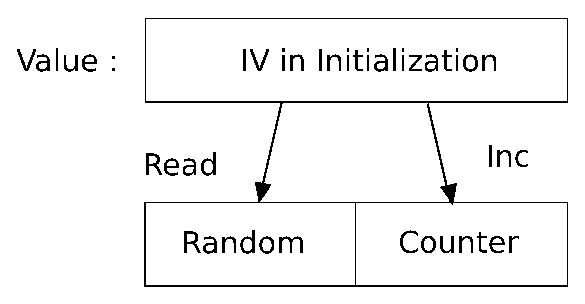
\includegraphics[scale=0.8]{./images/Nonce_Mixed_1}
\caption{The workflow of Nonce\_Mixed\_1.}
\end{figure}
\subsubsection*{Generic Part}
\begin{lstlisting}{}
generic
  Counter_Size: Positive := Block'Size / 16;
  with function To_Block_Type(Byte_Array:in Crypto.Types.Bytes)
   								return Crypto.Types.Nonces.Block;
  with function To_Bytes(Block: in Crypto.Types.Nonces.Block)
    								return Crypto.Types.Bytes;
\end{lstlisting}

%%%%%%%%%%%%%%%%%%%%%%%%%%%%%%%%%%%%%%%%%%%%%%%%%%%%%%%%%%%%%%%%%

\subsubsection*{Types}
\begin{lstlisting}{}
  type Nonce_Mixed_1 is new N.Nonce with private;
\end{lstlisting}

%%%%%%%%%%%%%%%%%%%%%%%%%%%%%%%%%%%%%%%%%%%%%%%%%%%%%%%%%%%%%%%%%

\subsubsection*{Procedures}
\begin{lstlisting}{}
  procedure Initialize(This : in out Nonce_Mixed_1; IV : in N.Block);
\end{lstlisting}
This procedure sets IV as the start value for the counter.

\hhline
\begin{lstlisting}{}
  overriding
  function Update(This : in out Nonce_Mixed_1) return N.Block;
\end{lstlisting}
This function increments the counter by one and stores the counter in
the second half of the nonce value. Then, it generates a new random
value and returns the concatenation: (half random and half counter)
random $\parallel$ counter.


%%%%%%%%%%%%%%%%%%%%%%%%%%%%%%%%%%%%%%%%%%%%%%%%%%%%%%%%%%%%%%%%%

\subsection*{Nonces\_Mixed\_2}
In this mixed solution, the initial vector IV will be stored to check
overflow. It separates the generation process into two steps. The
first step is the assignment of a random value to the first part of
the nonce. The second step is the update of the counter. At the end of
the update it checks the counter. If the counter overflows, then the
first step will be called once more. Figure \ref{Nonce2} shows how a
value of Nonces\_Mixed\_2 is generated.
\begin{figure}[h]
\centering
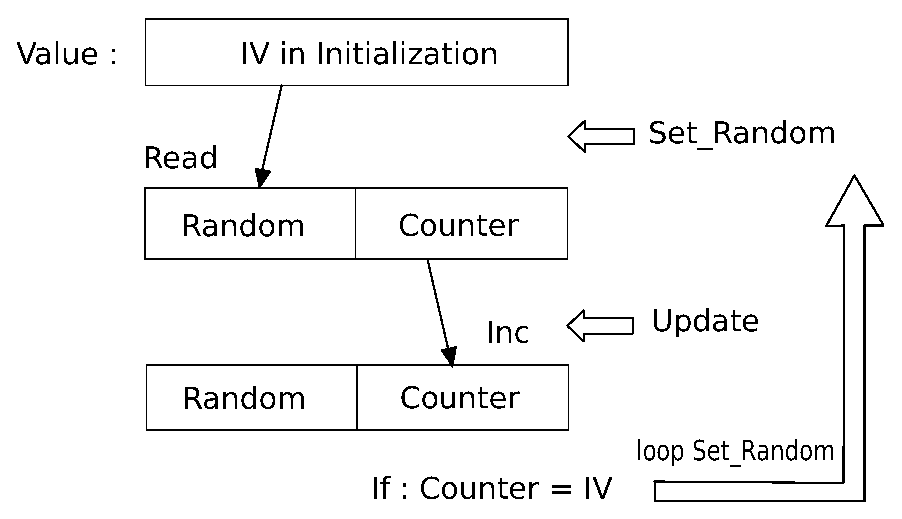
\includegraphics[scale=0.9]{./images/Nonce_Mixed_2}
\caption{The workflow of Nonces\_Mixed\_2.}\label{Nonce2}
\end{figure}

%%%%%%%%%%%%%%%%%%%%%%%%%%%%%%%%%%%%%%%%%%%%%%%%%%%%%%%%%%%%%%%%%

\subsubsection*{Generic Part}
\begin{lstlisting}{}
generic
  Counter_Size: Positive := Block'Size / 16;
  with function To_Block_Type(Byte_Array:in Crypto.Types.Bytes)
    								return Crypto.Types.Nonces.Block;
  with function To_Bytes(Block: in Crypto.Types.Nonces.Block)
    								return Crypto.Types.Bytes;
\end{lstlisting}

%%%%%%%%%%%%%%%%%%%%%%%%%%%%%%%%%%%%%%%%%%%%%%%%%%%%%%%%%%%%%%%%%

\subsubsection*{Types}
\begin{lstlisting}{}
  type Nonce_Mixed_2 is new N.Nonce with private;
\end{lstlisting}

%%%%%%%%%%%%%%%%%%%%%%%%%%%%%%%%%%%%%%%%%%%%%%%%%%%%%%%%%%%%%%%%%

\subsubsection*{Procedures}
\begin{lstlisting}{}
  procedure Initialize(This : in out Nonce_Mixed_2; IV : in N.Block);
\end{lstlisting}
It does the initialization and calls an internal procedure
\texttt{Set\_Random()} to generate a random value and store it in the
first half of the block. IV is assigned to the second half.

\hhline
\begin{lstlisting}{}
  overriding
  function Update(This : in out Nonce_Mixed_2) return N.Block;
\end{lstlisting}
The function \texttt{Update()} calls an internal function
\texttt{Inc()}, which increments the counter by one and stores the
counter in the second half of the block.

%%%%%%%%%%%%%%%%%%%%%%%%%%%%%%%%%%%%%%%%%%%%%%%%%%%%%%%%%%%%%%%%%%%
%%%%%%%%%%%%%%%%%%%%%%%%%%%%%%%%%%%%%%%%%%%%%%%%%%%%%%%%%%%%%%%%%%%
\newpage
\section{Example}
\subsubsection*{Nonce\_Ctr}
\begin{lstlisting}{}
  with Crypto.Types.Nonces;
  with Crypto.Types.Nonces.Nonces_Ctr;
  with Ada.Text_IO;
  with Ada.Directories;
  procedure Example_Nonces_Ctr is
    subtype Block is Natural range 0..255;
    function Inc(Item: Block) return Block is
         Result: Block := Item;
       begin
         Result := Result + 1;
         return Result;
    end Inc;
    package N is new Crypto.Types.Nonces(Block => Block);
    package Counter is new N.Nonces_Ctr(Inc => Inc);
    Nonce: Counter.Nonce_Ctr;
    B: Block := 0;
    Result : array(0..99) of Block;
    Distinct : Boolean := True;
  begin
    Counter.Initialize(This      => Nonce,
                       File_Path => "last_nonce.txt",
                       IV        => B);
    for i in Result'Range loop
        Result(i) := Counter.Update(Nonce);
    end loop;
    Counter.Finalize(Nonce);
    for i in Result'Range loop
        for j in (i+1)..Result'Last loop
            if Result(i) = Result(j) then
               Distinct := false;
            end if;
         end loop;
    end loop;
    Ada.Directories.Delete_File("last_nonce.txt");
    Ada.Text_IO.Put_Line(Distinct'Img);
  end Example_Nonces_Ctr;
\end{lstlisting}

%%%%%%%%%%%%%%%%%%%%%%%%%%%%%%%%%%%%%%%%%%%%%%%%%%%%%%%%%%%%%%%%%%%

\subsubsection*{Nonces\_Random}
\begin{lstlisting}{}
  with Crypto.Types.Nonces;
  with Crypto.Types.Nonces.Nonces_Random;
  with Crypto.Types; use Crypto.Types;
  with Ada.Text_IO;
  procedure Example_Nonces_Random is
     package N is new Crypto.Types.Nonces(Crypto.Types.B_Block128);
     package Rand is new N.Nonces_Random(Crypto.Types.To_B_Block128);
     Nonce: Rand.Nonce_Rand;
     Byte_Array: Crypto.Types.B_Block128 := (others => 0);
     Result : array(0..99) of Crypto.Types.B_Block128;
     Distinct : Boolean := True;
  begin
     for i in Result'Range loop
         Result(i) := Rand.Update(Nonce);
     end loop;
     for i in Result'Range loop
         for j in (i+1)..Result'Last loop
             if Result(i) = Result(j) then
                  Distinct := false;
             end if;
         end loop;
     end loop;
     Ada.Text_IO.Put_Line(Distinct'Img);
  end Example_Nonces_Random;
\end{lstlisting}

\chapter{Crypto.Symmetric}
\section{Funktion}
Dies ist das Wurzelpaket f�r die symmetrische Kryptographie.
Dieses Paket erm�glicht dem symmetrischen Teil den direkten Zugriff auf 
\texttt{Crypto.Types}  und \texttt{Crypto.Random}. Diesen beiden Pakete
stellen grundlegende Typen und  Basisfunktionen f�r den symmetrischen Teil der
ACL zur Verf�gung.\\
 Das Herzst�ck der symmetrischen Krypographie bilden in der 
ACL Blockchiffren. In dem folgenden Abschnitt wird der Aufbau einer solchen
innerhalb der ACL erl�utert.
 
\section{Blockchiffren}
\subsubsection{Logischer Aufbau}
Eine Blockchiffre ist ein drei logische Schichten unterteilt. Wobei man
als Anwendungsprogrammierer nur die API der h�chsten Schicht verwenden sollte. 
Denn nur mit dieser API ist eine sicher Nutzung einer Blockchiffre garantiert.

\subsubsection{1. Schicht: Algorithmus}
Auf dieser Ebene befindet sich der nackte Algorithmus einer symmetrischen 
Chiffre. Die API der einzelnen Algorithmen ist identisch und dient als 
Schnittstelle f�r die Blockchiffen-Schicht.
Bei jedem  Algorithmus wird die Quelle auf der er beruht genannt.
Damit ist es m�glich sich mit Hilfe der Quelle von der Korrektheit der 
Implementierung zu �berzeugen. 
Es ist auf keinen Fall eine schlechte Idee dies auch zu tun. Mehrere 
Informationen zu den einzelnen Algorithmen und Chiffren erfahren Sie im 
n�chsten Kapitel.\\ \ \\
\textbf{Bemerkung:}\\
Verwenden sie die API dieser Schicht nur um eine Blockchiffre zu 
generieren. Verwenden Sie sie auf keinen Fall f�r einen anderen Zweck.
Es gibt kein Szenario in dem dies einen Sinn ergibt. 
Diese API dient wirklich nur als Schnittstelle f�r die 2. Schicht.


\subsubsection{2. Schicht: Blockchiffre}
Auf dieser Ebene wird aus einem Algorithmus eine Blockchiffre im unsicheren
ECB-Modus (Electronic Code Book) generiert.
Verwenden sie diese API nur, wenn Sie sich auch mit symmetrischen 
Blockchiffren auskennen.
Diese API dient eigentlich nur als Schnittstelle f�r die 3. Schicht.
In Kapitel \ref{block} wird beschrieben wie man aus einem Algorithmus 
eine Blockchiffre generiert.


\subsubsection{3. Schicht: Modus}
Diese Schicht versetzt eine Blockchiffre in einen vern�nftigen Modus. Es gibt 
verschiedene Modi f�r verschiedene Szenarien die alle ihre Vor- und Nachteile 
haben. Alle unterst�tzen Modi und deren Vor- und Nachteil werden in dem
Kapitel \ref{modus} ausf�hrlich beschrieben.

\begin{figure}
  \begin{center}
    \huge
    \begin{tabular}{|c @{\ } c|}\hline
      III. & Modus\\
      \hline
      II. & Blockchiffre\\
      \hline
      I. & Algorithmus\\
    \hline
    \end{tabular}
  \end{center}
\caption{Die 3-Schichten-Architektur einer symmetrischen (Block-)chiffre}
\end{figure}

\subsubsection{Bemerkung}
Mit dieser 3. Schichten Architektur ist es auch m�glich Strom-Chiffren zu
implementieren. Man muss dazu aus er 1. Ebene eine Prozedur zur Verf�gung
stellen die die n�chsten n-Bit des Keystreams liefert. Damit kann man
eine Oneway-Blockchiffre (Kapitel \ref{oneblock}) konstruieren und diese in
den Oneway-OFB oder den Oneway-Counter-Modus versetzen. 
Im Moment beinhaltet die ACL  noch keinen Strom-Chiffre.
Es ist aber geplant die Strom-Chiffre Helix \cite{helix} zu implementieren.


\chapter{Crypto.Symmetric.Algorithm}\label{Algorithm}
All child packages of the package \texttt{Crypto.Symmetric.Algorithm}
are symmetric ciphers or hash functions. They have direct access to
individual operations, which use a cipher or a hash function. However
users should use the existing API.

%%%%%%%%%%%%%%%%%%%%%%%%%%%%%%%%%%%%%%%%%%%%%%%%%%%%%%%%%%%%%%%%%%%%%%
%%%%%%%%%%%%%%%%%%%%%%%%%%%%%%%%%%%%%%%%%%%%%%%%%%%%%%%%%%%%%%%%%%%%%%

\section{Symmetric Ciphers}
\subsubsection*{General}
The following procedures are defined and used within symmetric ciphers
of the ACL.
\begin{itemize}
\item One procedure \texttt{Prepare\_Key()}; it generates a cipher key
  from the delivered value.\\ \textbf{Example:}
\begin{lstlisting}{}
  procedure Prepare_Key(Key       : in  B_Block128;
                        Cipherkey : out Cipherkey_Type);
\end{lstlisting}
\item One procedure \texttt{Encrypt()}; it converts the input
  plaintext into a output ciphertext.\\

\noindent\textbf{Example:}
\begin{lstlisting}{}
  procedure Encrypt(Cipherkey  : in  Cipherkey_Type;
                    Plaintext  : in  B_Block128;
                    Ciphertext : out B_Block128);
\end{lstlisting}
\item One procedure \texttt{Decrypt()}; it recovers the input
 ciphertext to associated plaintext.\\

\noindent\textbf{Example:}
\begin{lstlisting}{}
  procedure Decrypt(Cipherkey  : in  Cipherkey_Type;
                    Ciphertext : in  B_Block128;
                    Plaintext  : out B_Block128);
\end{lstlisting}
\end{itemize}

%%%%%%%%%%%%%%%%%%%%%%%%%%%%%%%%%%%%%%%%%%%%%%%%%%%%%%%%%%%%%%%%%%%
%%%%%%%%%%%%%%%%%%%%%%%%%%%%%%%%%%%%%%%%%%%%%%%%%%%%%%%%%%%%%%%%%%%

\subsection{AES}\label{AES}
Advanced Encryption Standard (AES) is one of the best-known ciphers
which was officially standardized by the U.S. National Institute of
Standards and Technology (NIST) in 2001 \cite{AES-FIPS}.  Originally
it was called Rijndael, the name was a combination of the names of the
two inventors, Joan Daemen and Vincent Rijmen. The AES algorithm has a
fixed block size of 128 bits and a key size of 128, 192, or 256 bits.
During the AES algorithm, the input plaintext will be transformed
through a round transformation function 10, 12 or 14 times depending
on its key length, and the final output is the ciphertext
\cite{AES-FIPS}. The number of cycles of repetition are as follows:
\begin{itemize}
\item 10 rounds of repetition for 128 bit keys.
\item 12 rounds of repetition for 192 bit keys.
\item 14 rounds of repetition for 256 bit keys.
\end{itemize}
\subsubsection*{API of AES with 128 bit keys:}
\begin{lstlisting}{}
  type Cipherkey_AES128 is private;
  procedure Prepare_key128(Key       : in  B_Block128;
                           Cipherkey : out Cipherkey_AES128);
  procedure Encrypt128(Cipherkey  : in  Cipherkey_AES128;
                       Plaintext  : in  B_Block128;
                       Ciphertext : out B_Block128);
  procedure Decrypt128(Cipherkey  : in  Cipherkey_AES128;
                       Ciphertext : in  B_Block128;
                       Plaintext  : out B_Block128);
\end{lstlisting}
\subsubsection*{API of AES with 192 bit keys:}
\begin{lstlisting}{}
  type Cipherkey_AES192 is private;
  procedure Prepare_key192(Key       : in  B_Block192;
                           Cipherkey : out Cipherkey_AES192);
  procedure Encrypt192(Cipherkey  : in  Cipherkey_AES192;
                       Plaintext  : in  B_Block128;
                       Ciphertext : out B_Block128);
  procedure Decrypt192(Cipherkey  : in  Cipherkey_AES192;
                       Ciphertext : in  B_Block128;
                       Plaintext  : out B_Block128);
\end{lstlisting}

\subsubsection*{API of AES with 256 bit keys:}
\begin{lstlisting}{}
  type Cipherkey_AES256 is private;
  procedure Prepare_key256(Key       : in  B_Block256;
                           Cipherkey : out Cipherkey_AES256);
  procedure Encrypt256(Cipherkey  : in  Cipherkey_AES256;
                       Plaintext  : in  B_Block128;
                       Ciphertext : out B_Block128);
  procedure Decrypt256(Cipherkey  : in  Cipherkey_AES256;
                       Ciphertext : in  B_Block128;
                       Plaintext  : out B_Block128);
\end{lstlisting}

%%%%%%%%%%%%%%%%%%%%%%%%%%%%%%%%%%%%%%%%%%%%%%%%%%%%%%%%%%%%%%%%%%
%%%%%%%%%%%%%%%%%%%%%%%%%%%%%%%%%%%%%%%%%%%%%%%%%%%%%%%%%%%%%%%%%%

\subsection{Blowfish}
Blowfish was designed in 1993 by Bruce Schneier. It uses a key of
variable length (here the length 128-bit is used) and a 64-bit block
cipher. Blowfish has a key-expansion part and a part of 16-round
Feistel network for data encryption \cite{DBLP:conf/fse/Schneier93}.
\subsubsection*{API of Blowfish:}
\begin{lstlisting}{}
  type Cipherkey_Blowfish128 is private;
  subtype B_Block is Bytes;
  procedure Prepare_Key128(Key      :in  B_Block128;
                          Cipherkey :out Cipherkey_Blowfish128);
  procedure Encrypt128 (Cipherkey  : in  Cipherkey_Blowfish128;
                        Plaintext  : in  B_Block64;
                        Ciphertext : out B_Block64);
  procedure Decrypt128 (Cipherkey  : in  Cipherkey_Blowfish128;
                        Ciphertext : in  B_Block64;
                        Plaintext  : out B_Block64);
\end{lstlisting}

%%%%%%%%%%%%%%%%%%%%%%%%%%%%%%%%%%%%%%%%%%%%%%%%%%%%%%%%%%%%%%%%%%
%%%%%%%%%%%%%%%%%%%%%%%%%%%%%%%%%%%%%%%%%%%%%%%%%%%%%%%%%%%%%%%%%%

\subsection{Serpent}
Serpent is designed for 128-bit block ciphers, and was one of the five
finalists in the Advanced Encryption Standard (AES) contest. If you
put a high value on security and not such a high value on performance,
then you can try this block cipher. The implementation is based on the
Ada-Reference-Implementation by Markus G. Kuhn. Temporarily there is
only API for 256-bit cipher key. API for 128-bit and 192-bit keys is
in planning.
\subsubsection*{API of Serpent:}
\begin{lstlisting}{}
  type Cipherkey_Serpent256 is private;
  procedure Prepare_Key256(Key       : in  B_Block256;
                           Cipherkey : out Cipherkey_Serpent256);
  procedure Encrypt256(Cipherkey  : in  Cipherkey_Serpent256;
                       Plaintext  : in  B_Block128;
                       Ciphertext : out B_Block128);
  procedure Decrypt256(Cipherkey  : in  Cipherkey_Serpent256;
                       Ciphertext : in  B_Block128;
                       Plaintext  : out B_Block128);
\end{lstlisting}

%%%%%%%%%%%%%%%%%%%%%%%%%%%%%%%%%%%%%%%%%%%%%%%%%%%%%%%%%%%%%%%%%%
%%%%%%%%%%%%%%%%%%%%%%%%%%%%%%%%%%%%%%%%%%%%%%%%%%%%%%%%%%%%%%%%%%
\subsection{Triple DES(3DES, TDES, TDEA)}
Triple DES is the common name for the Triple Data Encryption Algorithm
(TDEA or Triple DEA), which applies the Data Encryption Standard (DES)
algorithm to each data block three times, and a TDES key is made of
three DES keys \cite{DES-FIPS}. The 192-bit key is decomposed before
encryption in three 64-bit keys. Due to that DES is software-relative
slow, TDES is the slowest block cipher. It is assumed that this cipher
can not be broken, because DES is over 20 years studied by the best
cryptoanalysts on its weakness. The idea comes from the book
\texttt{Applied Cryptography} by Burce
Scheier\footnote{http://www.schneier.com/book-applied.html, Dec
  2012.}.
\subsubsection*{API of Triple DES:}
\begin{lstlisting}{}
  type Cipherkey_TDES is private;
  procedure Prepare_Key(Key       : in  B_Block192;
                        Cipherkey : out Cipherkey_TDES);
  procedure Encrypt(Cipherkey  : in  Cipherkey_TDES;
                    Plaintext  : in  B_Block64;
                    Ciphertext : out B_Block64);
  procedure Decrypt(Cipherkey  : in  Cipherkey_TDES;
                    Ciphertext : in  B_Block64;
                    Plaintext  : out B_Block64);
\end{lstlisting}
\newpage
%%%%%%%%%%%%%%%%%%%%%%%%%%%%%%%%%%%%%%%%%%%%%%%%%%%%%%%%%%%%%%%%%
%%%%%%%%%%%%%%%%%%%%%%%%%%%%%%%%%%%%%%%%%%%%%%%%%%%%%%%%%%%%%%%%%
\subsection{Twofish}
Twofish is one of the five finalists of the Advanced Encryption
Standard contest, with a block size of 128 bits and a key of length up
to 256 bits. It uses the 16-round Feistel network with a bijective F
function, a transform, a bitwise rotation and a key schedule
\cite{Twofish}. The implementation is based on the C-Reference
implementation by Niels Ferguson and the twofish
specification\footnote{http://www.schneier.com/twofish.html}. In the
ACL it is implemented with 128, 192 or 256 bit keys.
\subsubsection*{API of Twofish with 128 bit keys:}
\begin{lstlisting}{}
  type Cipherkey_Twofish is private;
  subtype Cipherkey_Twofish128 is Cipherkey_Twofish;
  procedure Prepare_Key128(Key      : in  B_Block128;
                           Cipherkey: out Cipherkey_Twofish128);
  procedure Encrypt128(Cipherkey    : in  Cipherkey_Twofish128;
                       Plaintext    : in  B_Block128;
                       Ciphertext   : out B_Block128);
  procedure Decrypt128(Cipherkey    : in  Cipherkey_Twofish128;
                       Ciphertext   : in  B_Block128;
                       Plaintext    : out B_Block128);
\end{lstlisting}
\subsubsection*{API of Twofish with 192 bit keys:}
\begin{lstlisting}{}
  subtype Cipherkey_Twofish192 is Cipherkey_Twofish;
  procedure Prepare_Key192(Key      : in  B_Block192;
                          Cipherkey : out Cipherkey_Twofish192);
  procedure Encrypt192(Cipherkey    : in  Cipherkey_Twofish192;
                       Plaintext    : in  B_Block128;
                       Ciphertext   : out B_Block128);
  procedure Decrypt192(Cipherkey    : in  Cipherkey_Twofish192;
                       Ciphertext   : in  B_Block128;
                       Plaintext    : out B_Block128);
\end{lstlisting}
\subsubsection*{API of Twofish with 256 bit keys:}
\begin{lstlisting}{}
  subtype Cipherkey_Twofish256 is Cipherkey_Twofish;
  procedure Prepare_Key256(Key      : in  B_Block256;
                           Cipherkey: out Cipherkey_Twofish256);
  procedure Encrypt256(Cipherkey    : in  Cipherkey_Twofish256;
                       Plaintext    : in  B_Block128;
                       Ciphertext   : out B_Block128);
  procedure Decrypt256(Cipherkey    : in  Cipherkey_Twofish256;
                       Ciphertext   : in  B_Block128;
                       Plaintext    : out B_Block128);
\end{lstlisting}

%%%%%%%%%%%%%%%%%%%%%%%%%%%%%%%%%%%%%%%%%%%%%%%%%%%%%%%%%%%%%%%%%
%%%%%%%%%%%%%%%%%%%%%%%%%%%%%%%%%%%%%%%%%%%%%%%%%%%%%%%%%%%%%%%%%

\section{Hash Functions}\label{AlgorithmHash}
The iterative hash functions in the ACL can be called through a
Low-Level-API or High-Level-API.
\subsubsection*{Excursion: Iterative Hash Functions}
An iterative hash function $H$ decomposes a message $M$ into $r$
message blocks $m_i$ ($1\leq i \leq r$) of length $n$. All message
blocks will be hashed sequentially. To generate a hash value $h$ for
the complete message $M$, the intermediate outputs are also inputs for
the next round.  In general there exists: $h_i:= H(m_i,h_{i-1})$. For
$i=1$, $h_1:=H(M_1,h_0)$ will be applied, hereby $h_0$ is an initial
value, and will be initialized at the beginning. Messages whose length
is not multiple of $n$ will be inflated by a function
\texttt{Padding()} before encryption until the length is multiple of
$n$.

\subsubsection*{High-Level-API}
The High-Level-API is made of 3 procedures, which calculate hash value
of messages in string, bytes or file names in
string.\\

\noindent\textbf{Example:}
\begin{lstlisting}{}
  procedure Hash  (Message  : in String; Hash_Value: out W_Block160);
  procedure Hash  (Message  : in Bytes;  Hash_Value: out W_Block160);
  procedure F_Hash(Filename : in String; Hash_Value: out W_Block160);
\end{lstlisting}

\subsubsection*{Low-Level-API}
The Low-Level-API of a hash function has:
\begin{itemize}
\item One procedure \texttt{Init()}; it initializes the hash context (\texttt{This}).\\
\textbf{Example:}
\begin{lstlisting}{}
	procedure Init(This 		: in out Hash_Interface);
\end{lstlisting}
\item One procedure \texttt{Round()}; a message block (not the last block) will be hashed.\\
\textbf{Example:}
\begin{lstlisting}{}
	procedure Round(This 					: in out 	Hash_Interface;
                  Message_Block : in 		  W_Block512);
\end{lstlisting}
\item One function \texttt{Final\_Round()}; the last message block
  (\texttt{Last\_Message\_Block}) will be inflated and the final hash
  value is returned. Because of the \texttt{Padding()} function, the
  length of the last message block in byte (Last\_Message\_Length)
  should be passed as a parameter.\\

\noindent\textbf{Example:}
\begin{lstlisting}{}
 function Final_Round(This 		    : in out Hash_Interface;
										Last_Message_Block  : W_Block512;
										Last_Message_Length : Message_Block_Length512)
										return W_Block160;
\end{lstlisting}
\end{itemize}

\subsection{SHA-1}\label{SHA-1}
SHA-1 is a cryptographic hash function for 160-bit message blocks. SHA
stands for "Secure Hash Algorithm". SHA-1 was one of the most widely
used hash functions. In 2005, security flaws were identified in SHA-1
by X. Wang, Y.L. Yin und H.Yu, namely that a mathematical weakness
might exist \cite{DBLP:conf/crypto/WangYY05a}. Due to this new
discovery, it is now not advisable to use this hash function. The only
reason why the ACL supports this kind of hash function is its
tremendous degree of process in standard protocols such as digital
signature standard. But this hash function is expected to be no more
supported by the ACL, so you'd better use other hash functions if
possible. \\ \textbf{Remark:}\\ The performance of SHA-1 is slower
than SHA-256.
\subsubsection*{API}
\begin{lstlisting}{}
  -- high level API
  procedure Hash(Message : in String ; Hash_Value : out W_Block160);
  procedure Hash(Message : in Bytes  ; Hash_Value : out W_Block160);
  procedure F_Hash(Filename: in String; Hash_Value : out W_Block160);
  -- low level API
	procedure Init(This 		: in out SHA1_Interface);
	procedure Round(This 	: in out 	SHA1_Interface;
								 Message_Block: in 		W_Block512);
	function Final_Round(This 		    : in out SHA1_Interface;
											Last_Message_Block  : W_Block512;
											Last_Message_Length : Message_Block_Length512)
											return W_Block160;
\end{lstlisting}
\textbf{Exceptions:}
\begin{itemize}
\item If the message length is greater than $2^{64}-1024$:\quad
  \texttt{SHA1\_Constraint\_Error}.
\item In the procedure \texttt{F\_Hash()}, if the file can not be
  opened:\quad\texttt{File\_Open\_Error}.
 \item In the procedure \texttt{F\_Hash()}, if the size of the read
   data is smaller than 0:\quad\texttt{File\_Read\_Error}.
\end{itemize}

%%%%%%%%%%%%%%%%%%%%%%%%%%%%%%%%%%%%%%%%%%%%%%%%%%%%%%%%%%%%%
\subsection{SHA-256}
SHA-256 is a cryptographic hash function with a 256-bit output (hash
value), and it is a member of SHA-2 family, which is based on
SHA-1. This hash family has a hash value in sufficient length and
makes significant changes in security compared to the SHA-1 hash
function. Since this hash family works with 8*32-bit words, its use in
32-bit processors worths a consideration. If possible, SHA-1 should be
replaced by this new generation of SHA-2 hash family.
\subsubsection*{API}
\begin{lstlisting}{}
  -- high level API
  procedure Hash(Message : in Bytes ; Hash_Value : out W_Block256);
  procedure Hash(Message : in String; Hash_Value : out W_Block256);
  procedure F_Hash(Filename: in String; Hash_Value : out W_Block256);
  -- low level API
	procedure Init(This 		: in out SHA256_Interface);
	procedure Round(This 	: in out 	SHA256_Interface;
								 Message_Block: in 		W_Block512);
	function Final_Round(This 		    : in out SHA256_Interface;
											Last_Message_Block  : W_Block512;
											Last_Message_Length : Message_Block_Length512)
											return W_Block256;\end{lstlisting}
\textbf{Exceptions:}
\begin{itemize}
\item If the message length is greater than $2^{64}-1024$:\quad
  \texttt{SHA256\_Constraint\_Error}.
\item In the procedure \texttt{F\_Hash()}, if the file can not be
  opened:\quad\texttt{File\_Open\_Error}.
\item In the procedure \texttt{F\_Hash()}, if the size of the read
  data is smaller than 0:\quad\texttt{File\_Read\_Error}.
\end{itemize}

%%%%%%%%%%%%%%%%%%%%%%%%%%%%%%%%%%%%%%%%%%%%%%%%%%%%%%%%%%%%%

\subsection{SHA-512}
SHA-512 is the safest member in SHA-2 hash family, which is defined in
Secure Hash
Standard\footnote{http://www.itl.nist.gov/fipspubs/fip180-1.htm}. It
works with 8*64-bit dwords and is therefore particularly suitable for
64-bit architectures. If you are searching for a very safe and
standardized hash function, then this hash function is probably the
one.

%%%%%%%%%%%%%%%%%%%%%%%%%%%%%%%%%%%%%%%%%%%%%%%%%%%%%%%%%%%%%

\subsubsection*{API}
\begin{lstlisting}{}
  -- high level API
  procedure Hash(Message : in Bytes;  Hash_Value : out DW_Block512);
  procedure Hash(Message : in String; Hash_Value : out DW_Block512);
  procedure F_Hash(Filename: in String; Hash_Value: out DW_Block512); 
  -- low level API
	procedure Init(This 		: in out Sha512_Interface);
	procedure Round(This 	: in out 	Sha512_Interface;
								 Message_Block: in 		DW_Block1024);
	function Final_Round(This 		    : in out Sha512_Interface;
											Last_Message_Block  : DW_Block1024;
											Last_Message_Length : Message_Block_Length1024)
											return DW_Block512;

\end{lstlisting}
\textbf{Exceptions:}
\begin{itemize}
\item If the message length is greater than
  $2^{128}-1024$:\quad\texttt{SHA2\_Constraint\_Error}.
\item In the procedure \texttt{F\_Hash()}, if the file can not be
  opened:\quad\texttt{File\_Open\_Error}.
\item In the procedure \texttt{F\_Hash()}, if the size of the read
  data is smaller than 0:\quad\texttt{File\_Read\_Error}.
\end{itemize}

%%%%%%%%%%%%%%%%%%%%%%%%%%%%%%%%%%%%%%%%%%%%%%%%%%%%%%%%%%%%%%%%

\subsection{SHA-384}
The SHA-384 hash function looks like SHA-512. The difference between
SHA-384 and SHA-512 comes in 2 points:
\begin{enumerate}
\item SHA-384 uses different initial values.
\item In the last round of SHA-384 the returned hash value will be  cut to 384 bits.
\end{enumerate}
Since this hash function uses internally a 512-bit hash value, it's
not compatible to the general API in
\texttt{Crypto.Symmetric.Hashfunction}. Hense this hash function
should be avoided using.
%%%%%%%%%%%%%%%%%%%%%%%%%%%%%%%%%%%%%%%%%%%%%%%%%%%%%%%%%%%%%%%%
\subsubsection*{API}
\begin{lstlisting}{}
  -- high level API
  procedure Hash(Message : in Bytes;  Hash_Value : out DW_Block384);
  procedure Hash(Message : in String; Hash_Value : out DW_Block384);
  procedure F_Hash(Filename: in String;Hash_Value : out DW_Block384);
  -- low level API
	procedure Init(This 		: in out SHA384_Interface);
	procedure Round(This 	: in out 	SHA384_Interface;
								 Message_Block: in 		DW_Block1024);
	function Final_Round(This 		    : in out SHA384_Interface;
											Last_Message_Block  : DW_Block1024;
											Last_Message_Length : Message_Block_Length1024)
											return DW_Block384;

\end{lstlisting}
\textbf{Exceptions:}
\begin{itemize}
\item If the message length is greater than
  $2^{128}-1024$:\quad\texttt{SHA2\_Constraint\_Error}.
\item In the procedure \texttt{F\_Hash()}, if the file can not be
  opened:\quad\texttt{File\_Open\_Error}.
\item In the procedure \texttt{F\_Hash()}, if the size of the read
  data is smaller than 0:\quad\texttt{File\_Read\_Error}.
\end{itemize}

%%%%%%%%%%%%%%%%%%%%%%%%%%%%%%%%%%%%%%%%%%%%%%%%%%%%%%%%%%%%%%%%

\subsection{Whirlpool}
Whirlpool is a 512-bit hash function which operates on messages less
than $2^{256}$ bits in length. Whirlpool isn't developed as the SHA-2
hash family by NSA (National Security Agency) but by two free
cryptographers, Vincent Rijmen and Paulo Barreto
\cite{Whirlpool}. Whirlpool is based on a substantially modified AES,
cause Vincent Rijmen is one of the AES (\ref{AES}) designers. If you
want a safer hash function and don't care about compatibility with the
american crypto-standard, then you should consider using Whirlpool.
\subsubsection*{API}
\begin{lstlisting}{}
  -- high level API
  procedure Hash(Message : in Bytes;  Hash_Value : out DW_Block512);
  procedure Hash(Message : in String; Hash_Value : out DW_Block512);
  procedure F_Hash(Filename   :in  String;
                   Hash_Value :out DW_Block512);
  -- low level API
	procedure Init(This 		: in out Whirlpool_Interface);
	procedure Round(This 	: in out 	Whirlpool_Interface;
								 Message_Block: in 		DW_Block512);
	function Final_Round(This 		    : in out Whirlpool_Interface;
											Last_Message_Block  : DW_Block512;
											Last_Message_Length : Message_Block_Length512)
											return DW_Block512;

\end{lstlisting}
\textbf{Exceptions:}
\begin{itemize}
\item If the message length is greater than $2^{256}-1024$:\quad
  \texttt{Whirlpool\_Constraint\_Error}.
\item In the procedure \texttt{F\_Hash()}, if the file can not be
  opened:\quad\texttt{File\_Open\_Error}.
\item In the procedure \texttt{F\_Hash()}, if the size of the read
  data is smaller than 0:\quad\texttt{File\_Read\_Error}.
\end{itemize}

\chapter{Crypto.Symmetric.Algorithm.Oneway}\label{onealg}

Jede symmetrische Chiffre und kryptographische Hashfunktion
hat ein Unterpaket \glqq Oneway \grqq. Bei diesem Paket handelt es sich um 
eine symmetrische Chiffre ohne Entschl�sslungsoperation.\\
Auch bei den Oneway-Algorithmen sollte sie davon Abstand nehmen die vorhanden
API direkt zu verwenden.\\ \ \\

\subsubsection{API}

Ein Oneway-Paket stellt dem Anwendungsprogrammierer folgende Typen und 
Operationen zur Verf�gung.


\begin{itemize} 
   \item Einen privaten Typ \textbf{Cipherkey\_Oneway} der deterministisch aus
     einem  Schl�ssel generiert wird. Mit dessen Hilfe  kann man 
     die  Verschl�sselungsfunktion des entsprechenden Paketes aufrufen.
   \item Eine Prozedur \textbf{Prepare\_Oneway\_Key} die aus einem Schl�ssel
     den zugeh�rigen Cipherkey erstellt.\\ \ \\
     \textit{Beispiel:}
     \begin{lstlisting}{}
procedure Prepare_Oneway_Key(Key       : in B_Block; 
                             Cipherkey : out Cipherkey_Oneway);
     \end{lstlisting}
     
   \item Eine Prozedur \textbf{Encrypt\_Oneway}. 
     Diese Prozedur verschl�sselte einen Klartext (Plaintext) mit Hilfe eines
     Cipherkeys in einen Chiffretext (Ciphertext).\\ \ \\
     \textit{Beispiel:}
     \begin{lstlisting}{}
 procedure Encrypt_Oneway(Cipherkey  : in  Cipherkey_Oneway;
                          Plaintext  : in  B_Block;
                          Ciphertext : out B_Block);
     \end{lstlisting}
\end{itemize}


\chapter{Crypto.Symmetric.Blockcipher}\label{Blockcipher}
In this generic package a block cipher is generated based on the
symmetric algorithms (Chapter \ref{Algorithm}). Users should always
use the API of the package, where a secure application can be ensured.
When one encrypts two identical plaintext blocks $P_1=P_2$ with the
same key, then two identical ciphertext blocks $C_1=C_2$ will be
produced. Thus the ciphertext can provide information about the
structure of the plaintext.
\section{API}
The API of a block cipher is mainly made of the following parts:
\begin{itemize}
\item One procedure \texttt{Prepare\_Key()}: it assigns a value as the
  cipher key.
\begin{lstlisting}{}
  procedure Prepare_Key(Key : in Key_Type);
\end{lstlisting}
\item One procedure \texttt{Encrypt()}: the procedure encrypts a
  plaintext block (with a key) to a ciphertext block.
\begin{lstlisting}{}
  procedure Encrypt(Plaintext: in Block; Ciphertext : out Block);
\end{lstlisting}
\item One procedure \texttt{Decrypt()}: the procedure recovers a
  ciphertext block (with a key) to a plaintext block.
\begin{lstlisting}{}
  procedure Decrypt(Ciphertext: in Block; Plaintext : out Block);
\end{lstlisting}
\end{itemize}
%%%%%%%%%%%%%%%%%%%%%%%%%%%%%%%%%%%%%%%%%%%%%%%%%%%%%%%%%%%%%%%%

\section{Generic Part}
\begin{lstlisting}{}
  type Block is private;
  type Key_Type is private;
  type Cipherkey_Type is private;
  with procedure Prepare_Key(Key       : in  Key_Type;
                             Cipherkey : out Cipherkey_Type) is <>;
  with procedure Encrypt(Cipherkey  : in  Cipherkey_Type;
                         Plaintext  : in  Block;
                         Ciphertext : out Block) is <>;
  with procedure Decrypt(Cipherkey  : in  Cipherkey_Type;
                         Ciphertext : in  Block;
                         Plaintext  : out Block) is <>;
  with function To_Key_Type
                (B : Crypto.Types.Bytes) return Key_Type is <>;
  with function To_Block_Type
                (B : Crypto.Types.Bytes) return Block is <>;
  with function Block_To_Bytes
                (B : Block) return Crypto.Types.Bytes is <>;
\end{lstlisting}
Since they are generic, they should be specified at first.\\

\noindent\textbf{Exceptions:}
\begin{itemize}
\item In the function \texttt{To\_Key\_Type()}, if the size of the
  data does not match the size of the key
  type:\quad\texttt{Constraint\_Error}.
\item In the function \texttt{To\_Block\_Type()}, if the size of the
  data does not match the size of the
  block:\quad\texttt{Constraint\_Error}.
\end{itemize}

%%%%%%%%%%%%%%%%%%%%%%%%%%%%%%%%%%%%%%%%%%%%%%%%%%%%%%%%%%%%%%%%

\noindent\textbf{Remarks.}
Users don't need to generate block ciphers from the symmetric
algorithms every time. They can use the following already built
blockciphers in the ACL.
\begin{itemize}
\item \texttt{Crypto.Symmetric.Blockcipher\_AES128/AES192/AES256}
\item \texttt{Crypto.Symmetric.Blockcipher\_Blowfish128}
\item \texttt{Crypto.Symmetric.Blockcipher\_Noob64}
\item \texttt{Crypto.Symmetric.Blockcipher\_Serpent256}
\item \texttt{Crypto.Symmetric.Blockcipher\_TripleDES}
\item \texttt{Crypto.Symmetric.Blockcipher\_Twofish128/Twofish192/Twofish256}
\end{itemize}

\chapter{Crypto.Symmetric.Oneway\_Blockcipher}\label{Oneway-Blockcipher}
With generic packages we can also generate a one-way block cipher with help of a one-way symmetric algorithm (chapter \ref{OnewayAlgo}) or a hash function (chapter \ref{Hash}).

By the one-way block cipher which is based on hash functions, the length of the key (at least 256 bits) will be chosen so that it is impossible to search the complete key space. For instance of an irreversible counter of 219 bits, it demands min. $10^{51}erg.$ to traverse all states, it corresponds the energy to deliver a typical supernova. Thus to traverse all states of a 256 bits counter, it needs min. energy of 64 milliarde supernoven. But the energy output of our sun is just only $1,21*10^{41}erg.$ one year \cite{DBLP:books/daglib/0021657}. So that such a one-way block cipher is as (in-)secure as the basic hash functions.
\section{Generic Part}
\begin{lstlisting}{}
  generic
    type Block is private;
    type Key_Type is private;
    type Cipherkey_Type is private;
    with procedure Prepare_Key(Key       : in  Key_Type;
                               Cipherkey : out Cipherkey_Type);
    with procedure Encrypt(Cipherkey  : in  Cipherkey_Type;
                           Plaintext  : in  Block;
                           Ciphertext : out Block);
    with function To_Block_Type (B : Crypto.Types.Bytes) 
    							    return Block is <>;
    with function Block_To_Bytes(B : Block) 
    							    return Crypto.Types.Bytes is <>;
\end{lstlisting}
The types should be specified before use. Furthermore, the API should be identical to the one-way algorithms.\\
\section{API}
The API of a one-way block cipher is made as in the following:
\begin{itemize}
\item One procedure \texttt{Prepare\_Key()}: it assigns a value as the cipher key.
\begin{lstlisting}{}
  procedure Prepare_Key(Key : in Key_Type);
\end{lstlisting}
\item One procedure \texttt{Encrypt()}: it encrypts a plaintext block to a ciphertext block under the cipher key.
\begin{lstlisting}{}
  procedure Encrypt(Plaintext: in Block; Ciphertext: out Block);
\end{lstlisting}
\item One function \texttt{To\_Block()}: to transform data of bytes into a block.
\begin{lstlisting}{}
  function To_Block(Byte_Array: Crypto.Types.Bytes) return Block;
\end{lstlisting}
\textbf{Exception:}\\ 
If the size of the data does not match the size of the block:\quad\texttt{Constraint\_Error}.
\item One function \texttt{To\_Bytes()}: to transform a block into bytes.
\begin{lstlisting}{}
  function To_Bytes(B : Block) return Crypto.Types.Bytes;
\end{lstlisting}
\end{itemize}
\section{Use in Example}
\begin{lstlisting}{}
  with Crypto.Types; use Crypto.Types;
  with Crypto.Symmetric.Oneway_Blockcipher;
  with Crypto.Symmetric.Algorithm.TripleDES.Oneway;
  procedure Generic_Oneway_TripleDES is
  use Crypto.Symmetric.Algorithm.TripleDES.Oneway;
    package Oneway_TripleDES is
      new Crypto.Symmetric.Oneway_Blockcipher
      (Block          => B_Block64,
       Key_Type       => B_Block192,
       Cipherkey_Type => Cipherkey_Oneway_TDES,
       Prepare_Key    => Prepare_Oneway_Key,
       Encrypt        => Encrypt_Oneway);
  begin
    ...
  end Generic_Oneway_TripleDES;
\end{lstlisting}
\textbf{Remarks:}\\
Users don't need to generate one-way block cipher every time. There exist already one-way block ciphers.
\begin{itemize}
\item \texttt{Crypto.Symmetric.Oneway\_Blockcipher\_AES128}
\item \texttt{Crypto.Symmetric.Oneway\_Blockcipher\_AES192}
\item \texttt{Crypto.Symmetric.Oneway\_Blockcipher\_AES256}
\item \texttt{Crypto.Symmetric.Oneway\_Blockcipher\_Blowfish128}
\item \texttt{Crypto.Symmetric.Oneway\_Blockcipher\_Serpent256}
\item \texttt{Crypto.Symmetric.Oneway\_Blockcipher\_TripleDES}
\item \texttt{Crypto.Symmetric.Oneway\_Blockcipher\_Twofish128}
\item \texttt{Crypto.Symmetric.Oneway\_Blockcipher\_Twofish192}
\item \texttt{Crypto.Symmetric.Oneway\_Blockcipher\_Twofish256}
\item \texttt{Crypto.Symmetric.Oneway\_Blockcipher\_Whirlpool}
\item \texttt{Crypto.Symmetric.Oneway\_Blockcipher\_SHA1}
\item \texttt{Crypto.Symmetric.Oneway\_Blockcipher\_SHA256}
\item \texttt{Crypto.Symmetric.Oneway\_Blockcipher\_SHA384}
\item \texttt{Crypto.Symmetric.Oneway\_Blockcipher\_SHA512}
\end{itemize}

\chapter{Crypto.Symmetric.Tweakable\_Blockcipher}
Supposed that $M=m_1m_2m_3$, after encryption of normal block cipher (Chpater \ref{Blockcipher}) we get $C=c_1c_2c_3$, and if $m_1=m_3$, it is obvious that $c_1=c_3$, where $c=E(K,m)$. Thus the ciphertext may provide information about the plaintext.\\
For this reason a new block cipher type is considered by using a tweak value in key preparation, encryption or decryption, briefly $c=E(K,T,M)$. The tweak serves for much the same purpose that an initial vector for the CBC mode. Then if we encrypt the same plaintext block $m_1=m_3$ with the same key but distinct tweak values, we'll get two ciphertexts $c_1\neq c_3$ with a probability:
\begin{itemize}
\item $Pr[E(K,T,M)=E(K,T',M')]\approx \frac{1}{2^n}$
\end{itemize}
with $T\neq T', M=M'$, and $n$ is the size of the block. \\
This package is specified in \texttt{Crypto.Symmetric.Tweakable\_Blockcipher}.
\section{API}
\subsubsection*{Generic Part}
\begin{lstlisting}{}
  generic
    type Block is private;
    type Key_Type is private;
    type Tweak_Type is private;
\end{lstlisting}
\subsubsection*{Type}
\begin{lstlisting}{}
  type TB_Interface is limited interface;
\end{lstlisting}
If an interface is limited then it must be stated explicitly. This package provides a set of abstract operations with the interface \texttt{TB\_Interface}.\\
The API is made of the following operations:
\begin{itemize}
\item One procedure \texttt{Key\_Setup()} prepares a key.
\begin{lstlisting}{}
  procedure Key_Setup(This : in out TB_Interface;
                      Key  : in     Key_Type) is abstract;
\end{lstlisting}
\item One function \texttt{Encrypt()} encrypts a plaintext with a tweak value.
\begin{lstlisting}{}
  function Encrypt(This       : in out TB_Interface;
                   Tweak      : in     Tweak_Type;
                   Plaintext  : in     Block) 
                   return Block is abstract;
\end{lstlisting}
\item One function \texttt{Decrypt()} decrypts a ciphertext with the tweak value.
\begin{lstlisting}{}
  function Decrypt(This       : in out TB_Interface;
                   Tweak      : in     Tweak_Type;
                   Ciphertext : in     Block) 
                   return Block is abstract;
\end{lstlisting}
\end{itemize}
\textbf{Notice that these operations are all abstract, they have no body and can never be called.} An implementation of the abstraction can be created by deriving a concrete type from the interface \texttt{TB\_Interface} and providing concrete operations for that implementation. Figure \ref{TweakBlock} shows the general structure of a tweakable blockcipher.
\begin{figure}[htp]
\centering
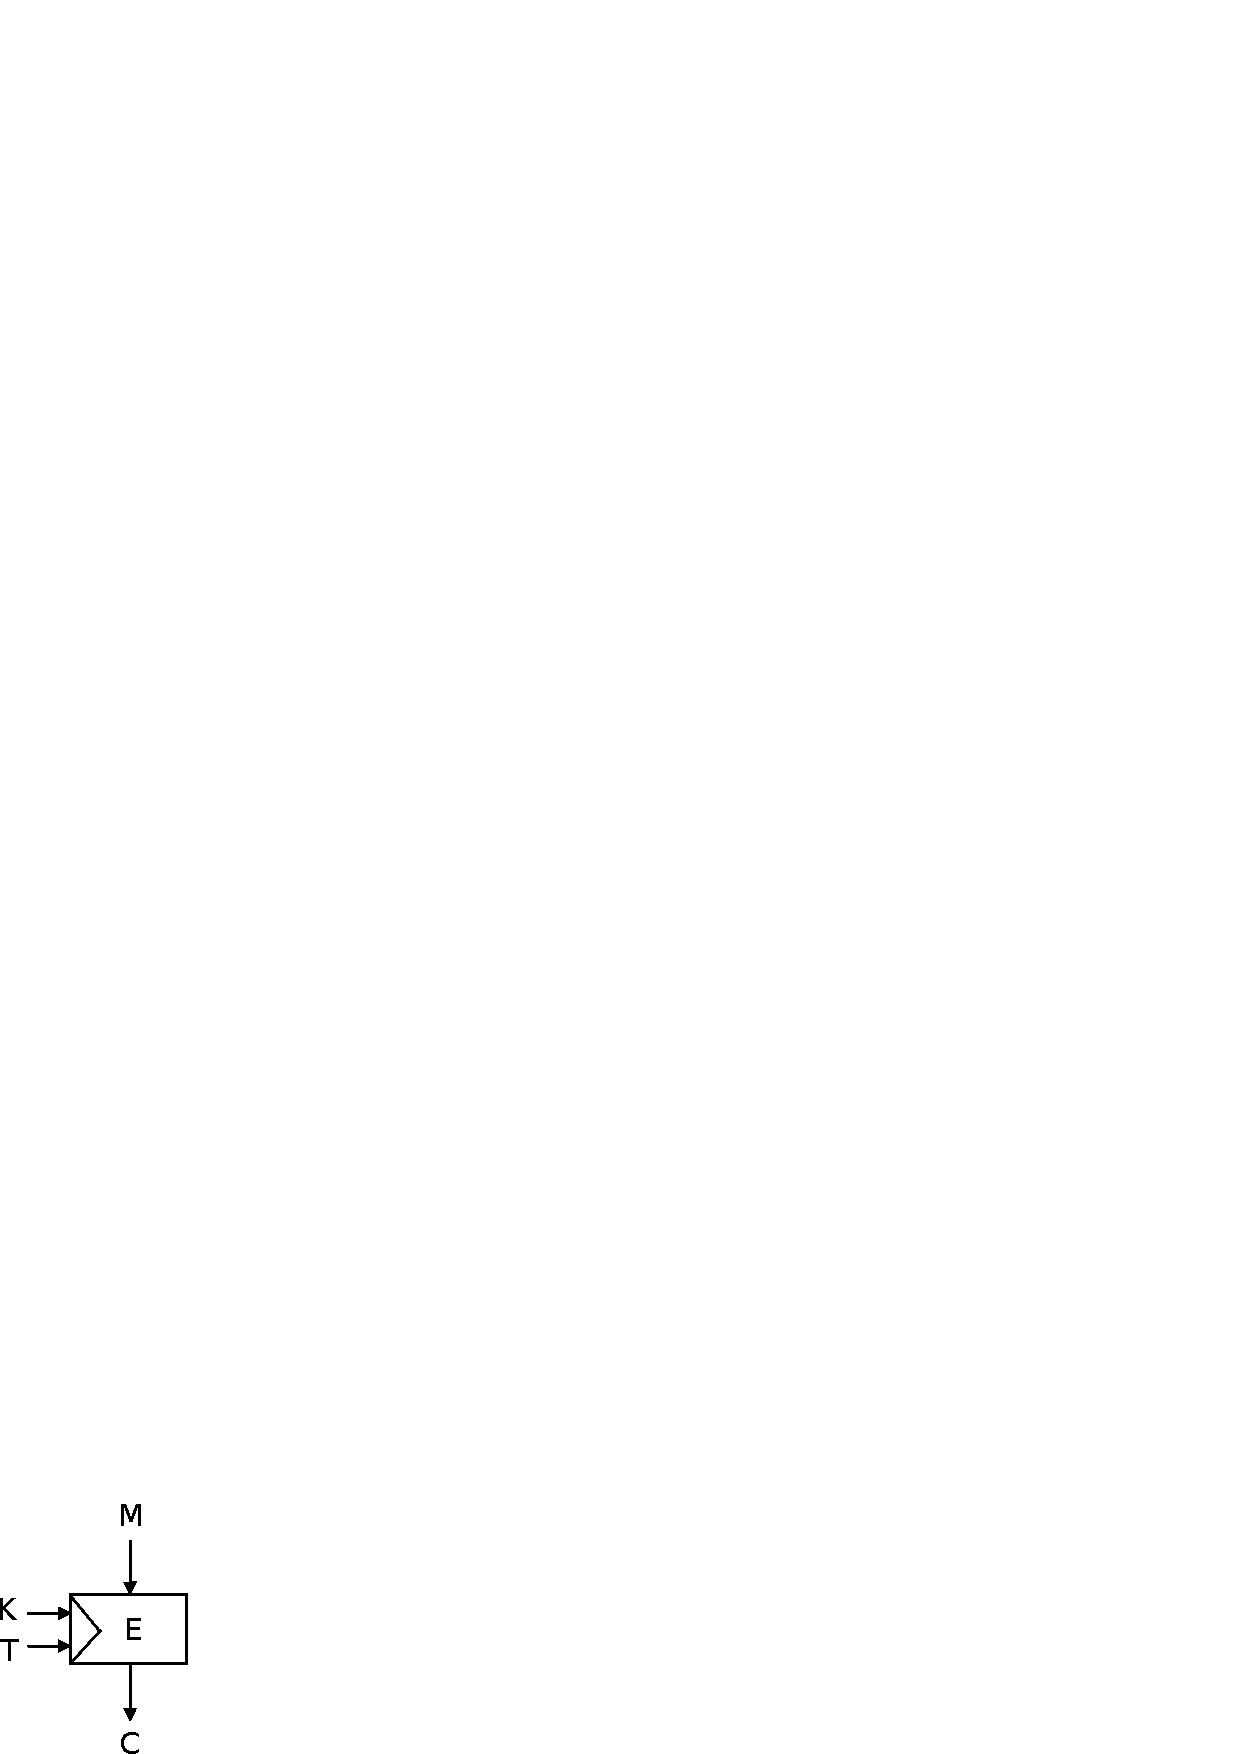
\includegraphics[scale=1]{Pictures/Tweak_BC.pdf} 
\caption{Structure of the tweakable blockcipher.}\label{TweakBlock}
\end{figure}
%%%%%%%%%%%%%%%%%%%%%%%%%%%%%%%%%%%%%%%%%%%%%%%%%%%%%%%%%%%%%%%%
%%%%%%%%%%%%%%%%%%%%%%%%%%%%%%%%%%%%%%%%%%%%%%%%%%%%%%%%%%%%%%%%
\section{Child Packages}
The ACL provides two instantiations of the tweakable block cipher. The two tweakable block cipher based implementations can be distinguished by the usage of the tweak value. The package \texttt{Tweakable\_Blockcipher\_TX} uses the tweak value in key preparation, while in the package \texttt{Tweakable\_Blockcipher\_CMT} the tweak value is used in encryption. Other instantiations of the tweakable block cipher will be provided in the future.
\subsection*{Tweakable\_Blockcipher\_TX}
\subsubsection*{Generic Part}
\begin{lstlisting}{}
  generic
    with package BC is new Crypto.Symmetric.Blockcipher(<>);
    with function To_Bytes(K : in BC.Key_Type) 
    								return Crypto.Types.Bytes;
\end{lstlisting}
\subsubsection*{Types}
\begin{lstlisting}{}
  package Tweakable_Blockciphers is new
   Crypto.Symmetric.Tweakable_Blockcipher(Block   	  => BC.Block,
														Key_Type   => BC.Key_Type,
														Tweak_Type => BC.Block);
   type TX is new Tweakable_Blockciphers.TB_Interface with private;
\end{lstlisting}
\subsubsection*{Procedures}
Concrete operations are provided here for the concrete type TX to implement the interface \texttt{TB\_Interface}.
We have to include the \texttt{overriding} indicator whenever we declare a further \texttt{Key\_Setup()}, \texttt{Encrypt()} or \texttt{Decrypt()}. This ensures that if we make a simple typographical error such as misspelling or getting the parameters wrong then the compiler will detect the error and not just add a bogus operation.
\begin{lstlisting}{}
  overriding
  procedure Key_Setup(This : in out TX; Key : in BC.Key_Type);
  overriding
  function Encrypt(This       : in out TX;
                   Tweak      : in     BC.Block;
                   Plaintext  : in     BC.Block) return BC.Block;
\end{lstlisting}
Function \texttt{Encrypt()} calls the procedure \texttt{Key\_Setup()} to combine the value \texttt{Tweak} and a user-defined key in order to generate a cipher key, and then encrypts the plaintext under the cipher key. By decryption it makes from the value \texttt{Tweak} a cipher key and then use this key to recover the ciphertext.
%%%%%%%%%%%%%%%%%%%%%%%%%%%%%%%%%%%%%%%%%%%%%%%%%%%%%%%%%%%%%%%%%%%%%%%%
%%%%%%%%%%%%%%%%%%%%%%%%%%%%%%%%%%%%%%%%%%%%%%%%%%%%%%%%%%%%%%%%%%%%%%%%
\subsection*{Tweakable\_Blockcipher\_CMT}
\subsubsection*{Generic Part}
\begin{lstlisting}{}
  generic
    with package BC is new Crypto.Symmetric.Blockcipher(<>);
    with function "xor"(Left, Right: BC.Block) return BC.Block is <>;
\end{lstlisting}
\subsubsection*{Types}
\begin{lstlisting}{}
  package Tweakable_Blockciphers is new
   Crypto.Symmetric.Tweakable_Blockcipher(Block      => BC.Block,
														Key_Type   => BC.Key_Type,
														Tweak_Type => BC.Block);
   type CMT is new Tweakable_Blockciphers.TB_Interface 
   											with null record;
\end{lstlisting}
Concrete operations should be provided for the new interface \texttt{CMT}.
\subsubsection*{Procedures}
\begin{lstlisting}{}
  overriding
  function Encrypt(This       : in out CMT;
                   Tweak      : in     BC.Block;
                   Plaintext  : in     BC.Block) return BC.Block;
\end{lstlisting}
In the procedure \texttt{Encrypt()} the encryption process will be made twice. After the first encryption the ciphertext is XORed with the value \texttt{Tweak} and then delivered as plaintext for the second time. In the procedure \texttt{Decrypt()} vice versa.\\
%%%%%%%%%%%%%%%%%%%%%%%%%%%%%%%%%%%%%%%%%%%%%%%%%%%%%%%%%%%%%%%%%%%%%%
%%%%%%%%%%%%%%%%%%%%%%%%%%%%%%%%%%%%%%%%%%%%%%%%%%%%%%%%%%%%%%%%%%%%%%
\section{Example}
\begin{lstlisting}{}
  with Crypto.Symmetric.Tweakable_Blockcipher_CMT;
  with Crypto.Symmetric.Blockcipher_AES128;
  with Crypto.Types;
  with Crypto.Types.Random;
  with Ada.Text_IO;
  procedure Example_TBC is
    package AES128 renames Crypto.Symmetric.Blockcipher_AES128;
    package CMT128 is new Crypto.Symmetric.Tweakable_Blockcipher_CMT
   					 (BC => AES128, "xor" => Crypto.Types."xor");
    use CMT128;
    use Crypto.Types;
    TB_CMT : CMT128.CMT;
    Key, P_1, P_2 : B_Block128;
    Ciphertext : B_Block128;
    Tweak_Value : B_Block128;
  begin
    Crypto.Types.Random.Read(P_1);
    Crypto.Types.Random.Read(Tweak_Value);
    Key_Setup(TB_CMT, Key);
    Ciphertext := Encrypt(TB_CMT, Tweak_Value, P_1);
    P_2 := Decrypt(TB_CMT, Tweak_Value, Ciphertext);
    if P_1 = P_2 then
       Ada.Text_IO.Put_Line("Same");
    end if;
  end Example_TBC;
\end{lstlisting}
\chapter{Crypto.Symmetric.Mode}\label{Mode}
With this package it is possible to work with a block cipher in a secure operating mode. Generally an operating mode integrates a block cipher with a feedback and some easy operations ($+,xor$), and will be initialized with a random start value (IV). Thus the ciphertext depends not only on plaintext and key, but also on the random start value. If man encrypts twice a plaintext with the same cipher key but different IVs, then man gets different ciphertexts. With the feedback that two same plaintext blocks will be encrypted to different ciphertext blocks, i.e. in an operating mode two plaintext blocks $P_1$ and $P_2$ with $P_1=P_2$ are encrypted, with absolute probability to two ciphertext blocks $C_1$ and $C_2$ with $C_1\neq C_2$. For this reason it is now possible to encrypt more messages securely under the same key.\\
\textbf{Remark: To decrypt a ciphertext, man needs the same key and IV which used in encryption.} One should always keep the IV with the related ciphertext. \textbf{The security of a mode is independent on the familarity of the start value.} Therefore it is in general, that man concatenates the ciphertext to the end of the start value to get the final output $C'$ ($C'=IV||C$). In this chapter several kinds of modes will be introduced.
\section{API}\label{API-Mode}
The API of a mode is made of four procedures.
\begin{itemize}
\item One procedure \texttt{Init()}; it initializes a mode by assigning a key and an initial value.
\begin{lstlisting}{}
  procedure Init(Key : in Key_Type; Initial_Value : in Block);
\end{lstlisting}
\item One procedure \texttt{Encrypt()}; 
\begin{lstlisting}{}
  procedure Encrypt(Plaintext: in Block; Ciphertext: out Block);
\end{lstlisting}
\item One procedure \texttt{Decrypt()};
\begin{lstlisting}{}
  procedure Decrypt(Ciphertext: in Block; Plaintext: out Block);
\end{lstlisting}
\item One procedure \texttt{Set\_IV()}; it assigns the start value. The mode should be reinitialized after every encryption or decryption (A message is made of $n$ plaintext blocks, which corresponds with $n$ calls of the \texttt{Encrypt()} or \texttt{Decrypt()} procedures).
\begin{lstlisting}{}
  procedure Set_IV(Initial_Value : in Block);
\end{lstlisting}
\end{itemize}
%%%%%%%%%%%%%%%%%%%%%%%%%%%%%%%%%%%%%%%%%%%%%%%%%%%%%%%%%
%%%%%%%%%%%%%%%%%%%%%%%%%%%%%%%%%%%%%%%%%%%%%%%%%%%%%%%%%
\section{Cipher Block Chaining Mode (CBC)}
\subsubsection*{Package: Crypto.Symmetric.Mode.CBC}
In the CBC mode, each block of plaintext will be XORed with the previous ciphertext block before being encrypted (for the first time XORed with an initial value). This way, each outputed ciphertext block depends on all plaintext blocks processed up to that point \cite{DBLP:reference/crypt/2011}. 
\subsubsection*{Encryption}
Mathematical description: $C_i=E_K(P_i\oplus C_{i-1})\,, C_0=IV$\,.\\
Figure \ref{CBCEN} shows the workflow of the CBC encryption.
By the initialization, the start value IV will be stored as $C_0$. A plaintext block $P_1$ is to encrypt, it will be XORed with $C_0$ and then encrypted to a ciphertext block $C_1$. The next plaintext block $P_2$ will XORed with $C_1$ and then encrypted to $C_2$ and so on.
\begin{figure}[h]
\centering
\includegraphics[scale=0.8]{Pictures/CBC_En.pdf}  
\caption{Workflow of the CBC encryption. Adapted from \cite{DBLP:reference/crypt/2011}.}\label{CBCEN}
\end{figure}
\subsubsection*{Decryption}
Mathematical description: $P_i=C_{i-1}\oplus D_K(C_i)$.\\
Figure \ref{CBCDE} shows the decryption workflow of CBC. It's the reverse of encryption. At the beginning the mode will be initialized with IV or in \texttt{Set\_IV()} reinitialized. A ciphertext block $C_1$ will be decrypted and the output will be XORed with $C_0$. The result of the XOR operation is the plaintext block $P_1$. The next ciphertext block $C_2$ will be decrypted and the output will be XORed with $C_1$ as $P_2$ and so on. 
\begin{figure}[h]
\centering
\includegraphics[scale=0.8]{Pictures/CBC_De.pdf} 
\caption{Workflow of the CBC decryption. Adapted from \cite{DBLP:reference/crypt/2011}.}\label{CBCDE}
\end{figure}
\subsubsection*{Purpose of Use}
\begin{itemize}
\item \textbf{Data Encryption}\\
Since there can be no error by synchronization in this mode, it is useful for data encryption. However it can lead to bit errors (through defective hardware or the like). One bit error in a ciphertext block $C_i$ can influence the plaintext block $P_i$ and also the related bit in next plaintext block $P_{i+1}$.
\item \textbf{Message Integrity Testing}\\
In order to test the integrity of a message, we encrypt the message and only need to remember two ciphertext blocks: $C_0=IV$ and $C_n$. The remaining ciphertext blocks are not required. Now we can certify at any time by encrypting the message $M$ to $C'_n$ with the start value $C_0$ and compare $C_n$ with $C'_n$, whether the message is changed or not. If $C_n=C'_n$, then the message $M$ is the original one, otherweise at least one of $IV$, $C_n$ or $M$ is changed. "Changed" is understood as accidental tipping of one or more bits.
\item \textbf{Message Authenticity Testing}\\
Supposed that you tell Alice a key, who you'd never met before. And one day you want to meet Alice to exchange secret data. To ensure that the people at the meeting point is really Alice, you bring a message $M$ and a randomly start value $IV$. You ask Alice to encrypt the message to $C'_n$ with the key and the start value. If $C'_n$ agrees with your computed $C_n$ (neither you nor Alice has told anyone the key), then the person is with significant propability to be Alice. If the two values are not the same, then the person is not Alice.
\item \textbf{Notice: The CBC-Mode is only secure when the exchanged messages are at the same length.} So users should pay attention to use the CBC Mode.
\end{itemize}
%%%%%%%%%%%%%%%%%%%%%%%%%%%%%%%%%%%%%%%%%%%%%%%%%%%%%%%%%
%%%%%%%%%%%%%%%%%%%%%%%%%%%%%%%%%%%%%%%%%%%%%%%%%%%%%%%%%
\section{BPS}
\subsubsection*{Package: Crypto.Symmetric.Mode.BPS}
BPS is a generic format-preserving symmetric encryption algorithm, which can cipher short or long string of characters from any given set, e.g. credit card numbers.
\subsubsection*{Encryption and Decryption}
The main process is similar to the CBC mode with an IV set to 0.
Internally a 8-round encryption is used. The plaintext will be divided into two sub-strings $L,R$ of similar length, i.e. $P=L||R$, and each of them will be updated in turn \cite{BPS}. Decryption is also composed of 8 rounds. They work as shown in Figure \ref{BPSED}.\\
\begin{figure}[htp]
\center
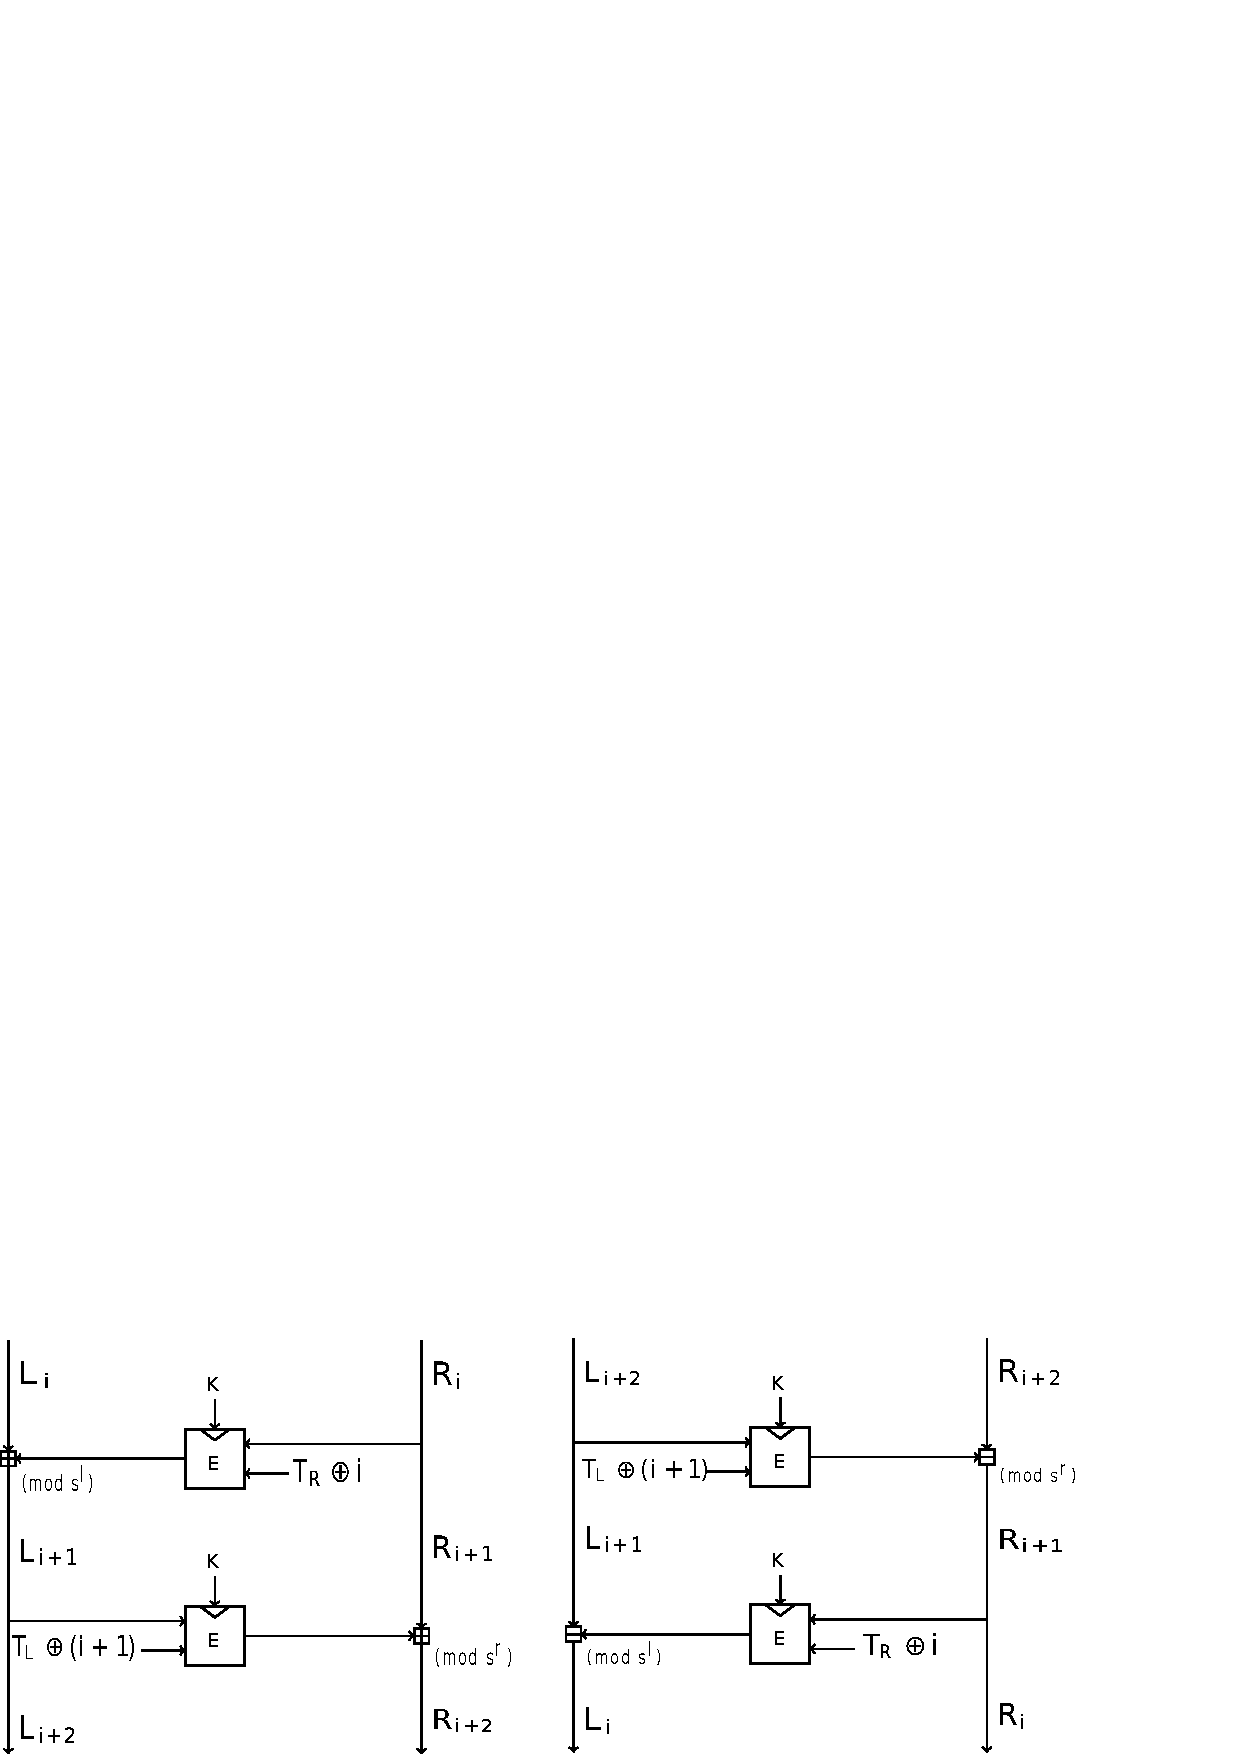
\includegraphics[scale=0.8]{Pictures/BPS_En_De.pdf} 
\caption{Workflow of the internal encryption (Left) and decryption (Right) in the BPS. \cite{BPS}}\label{BPSED}
\center
\end{figure}
\subsection*{Remarks}
\begin{itemize}
\item One advantage of BPS is its adaptability, all the block cipher and hash
function standardized primitives (TDES, AES or SHA-2) can be used as basic internal bricks \cite{BPS}. 
\item The internal tweak values is useful to avoid some kind of dictionary attacks \cite{BPS}. Indeed, if no tweak is used, a third party could build a dictionary of plaintext / ciphertext pairs and find with good probability the eavesdropped encrypted PANs (Personal Account Numbers), this attack works when the amount of data is small, which is particularly the case for an array of numbers encryption \cite{BPS}. "Using random tweak will render this dictionary technique useless as one dictionary per tweak value would be required" \cite{BPS}.
\item An essential quality of BPS is its efficiency. Due to that the input key for all the block cipher internal calls is constant, this requires only one internal cipher key per BPS encryption, which saves a lot of operations and time \cite{BPS}. Moreover, w = 8 rounds is recommanded, it makes the whole encryption process very efficient \cite{BPS}.
\end{itemize}
%%%%%%%%%%%%%%%%%%%%%%%%%%%%%%%%%%%%%%%%%%%%%%%%%%%%%%%%%
%%%%%%%%%%%%%%%%%%%%%%%%%%%%%%%%%%%%%%%%%%%%%%%%%%%%%%%%%
\section{Cipher Feedback Mode (CFB)}\label{CipherFeedbackMode}
\subsubsection*{Package: Crypto.Symmetric.Mode.CFB}
The cipher feedback (CFB) mode, a close relative of CBC, makes a block cipher into a self-synchronizing stream cipher \cite{DBLP:reference/crypt/2011}.
\begin{figure}[htp]
\center
\includegraphics[scale=0.8]{Pictures/CFB_En.pdf} 
\caption{Workflow of the CFB encryption. Adapted from \cite{DBLP:reference/crypt/2011}.}\label{CFBEN}
\center
\end{figure}\\
\subsubsection*{Encryption}
Mathematical description : $C_i=E_K(C_{i-1})\oplus P_i$, $C_0=IV$.\\
Figure \ref{CFBEN} shows the workflow of encryption in CFB. By initialization the start value IV will be stored as $C_0$. To encrypt a $n$ bit ($n<$ Block'Size) message, it will be copied in the plaintext block, and then padded with zeros. To encrypt a plaintext block $P_1$, the start value $C_0$ will be encrypted at first, and then XORed with $P_1$ and stored as $C_1$. Following plaintext blocks will be processed iteratively until the complete message is encrypted.
\subsubsection*{Decryption}
Mathematical description : $P_i=E_K(C_{i-1})\oplus C_i$, $C_0=IV$.\\
As shown in Figure \ref{CFBDE}, the decryption in CFB makes use of the encryption algorithm. At the beginning the mode will be initialized or through \texttt{Set\_IV()} reinitialized. To decrypt a ciphertext block $C_i$, $C_{i-1}$ will be decrypted at first and then XORed with $C_i$. The output of the operation is $P_i$.
\begin{figure}[h]
\centering
\includegraphics[scale=0.8]{Pictures/CFB_De.pdf} 
\caption{Workflow of the CFB decryption. Adapted from \cite{DBLP:reference/crypt/2011}.} \label{CFBDE}
\end{figure}
\subsubsection*{Remarks}
In comparison with CBC-Mode, which can be used when a complete data block exists, CFB-Mode can be used to encrypt not only data but also bytes (8-CFB). Therefore it is mainly used for encryption of byte streams (e.g. Remote shell).\\
In n-CFB-Mode:
\begin{itemize}
\item an error in plaintext will affect the following complete ciphertext and in decryption it goes backward.
\item an error in ciphertext $C_i$ will affect the plaintext block $P_i$ and also the following $\frac{m}{n}-1$ plaintext blocks, where $m$ is the size of the message.
\item An aggressor can change the message bits in the last ciphertext block without being found.
\end{itemize}
%%%%%%%%%%%%%%%%%%%%%%%%%%%%%%%%%%%%%%%%%%%%%%%%%%%%%%%%%
%%%%%%%%%%%%%%%%%%%%%%%%%%%%%%%%%%%%%%%%%%%%%%%%%%%%%%%%%
\section{Counter Mode (CTR)}\label{CounterMode}
\subsubsection*{Package: Crypto.Symmetric.Mode.CTR}
In Counter Mode the feedback isn't dependent on plaintext, but on a counter, which will be increased by 1 after every encryption. Note that the nonce in Figure \ref{CTREN} and Figure \ref{CTRDE} is the same thing as the initial vector (IV) in other graphs. 
\subsubsection*{Encryption}
Mathematical description : $C_i=P_i\oplus E_K(IV+i-1)$.\\
In Figure \ref{CTREN} the counter is initialized at first. The current counter $IV+i-1$ of each block is encrypted, the output is then XORed with plaintext block $P_i$, and the result is $C_i$.
\begin{figure}[h]
\centering
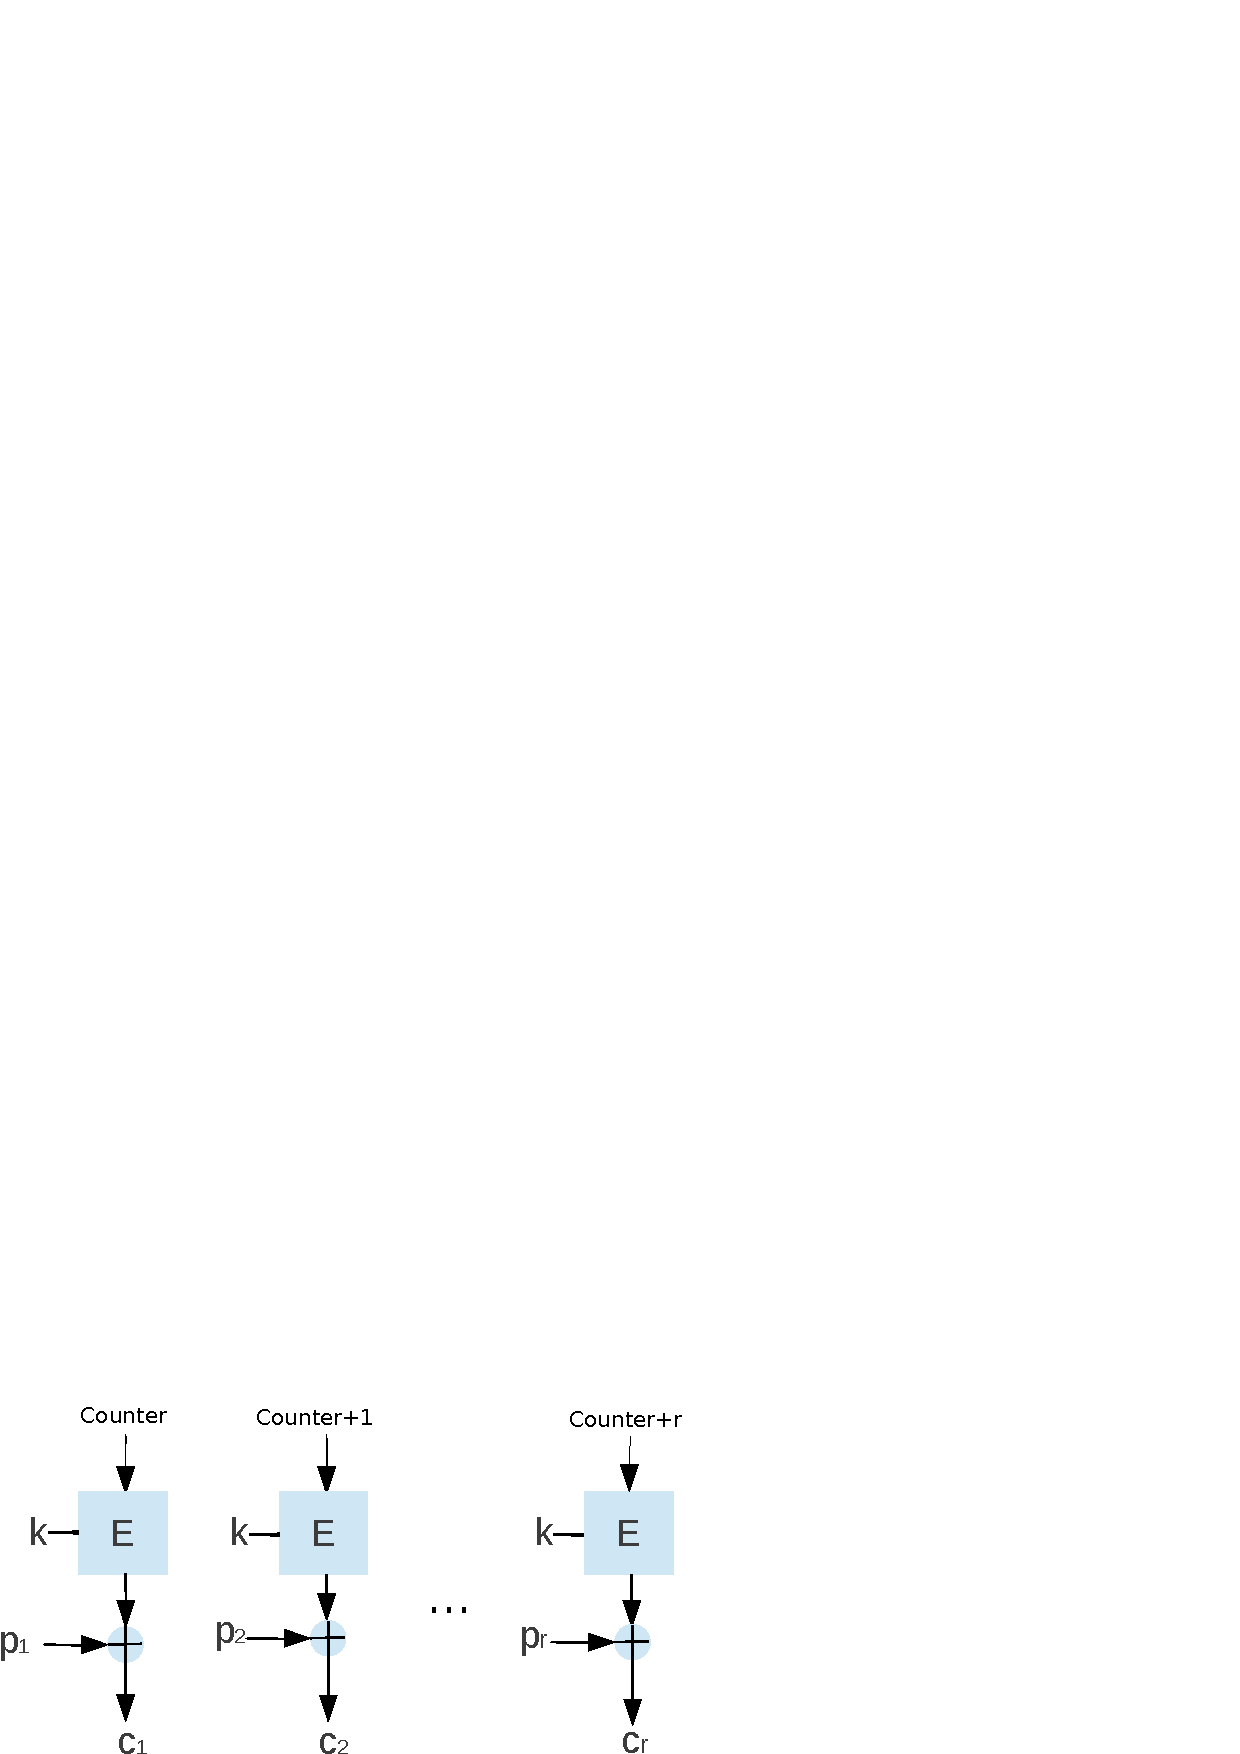
\includegraphics[scale=0.8]{Pictures/CTR_En.pdf} 
\caption{Workflow of the CTR encryption. Adapted from \cite{DBLP:reference/crypt/2011}.}\label{CTREN}
\end{figure}
\subsubsection*{Decryption}
Mathematical description : $P_i=C_i\oplus E_K(IV+i-1)$.\\
Note that in Figure \ref{CTRDE} the encryption algorithm is used in decryption.
After initialization counter $IV+i-1$ will be encrypted, then the output will be XORed with $C_i$ and the result is $P_i$. It is done iteratively until the last block.
\begin{figure}[h]
\centering
\includegraphics[scale=0.8]{Pictures/CTR_De.pdf} 
\caption{Workflow of the CTR decryption. Adapted from \cite{DBLP:reference/crypt/2011}.}\label{CTRDE}
\end{figure}
\subsubsection*{Remarks}
\begin{itemize}
\item \textbf{En-/Decryption of Messages with Random Access}\\
Since that the counter mode is used to decrypt individual ciphertext block, this procedure is suitable for decryption of data with random access e.g. Database.
\item \textbf{Parallel En-/Decryption}\\
Parallelization is possible when man calculates an interval from the start value (IV) and the length of the message is $L$: $[IV\cdots IV+L]$. The interval is decomposed in max. $L$ disjunktive part intervals. Then the message blocks in the part intervals can be en-/decrypted parallel.
\item \textbf{Phasic "High Speed" Encryption}\\
This is a professional function that based on "Low-Level-API" (\ref{Low-Level}) of CTR mode. Please use this only when you konw what it does. In CTR mode it is possible to generate random keystream bits without a message block to be needed. When you generate enough keystream bits with the CTR mode, then you are able to encrypt the messages very quickly through being XORed with the already produced keystream bits.
\end{itemize}
\subsubsection*{Notice:}
\begin{itemize}
\item A bit error in plaintext will influence only one bit in ciphertext and vice versa.
\item Manipulation on plaintext is clear, because every change in ciphertext influences directly the plaintext.
\item Error in Synchronization (Alice and Bob are in different counter states) can not be solved. 
\end{itemize}
\subsubsection*{Low-Level-API}\label{Low-Level}
This API can be used only when you know exactly what it does.
\begin{lstlisting}{}
  procedure Next_Block(Keystream : out Block);
\end{lstlisting}
Mathematical description : $C=E_K(Counter)$; $Counter:=Counter+1$.\\
It encrypts the internal counter to $C$, and the counter will be increased by 1.
%%%%%%%%%%%%%%%%%%%%%%%%%%%%%%%%%%%%%%%%%%%%%%%%%%%%%%%%%%%%%
%%%%%%%%%%%%%%%%%%%%%%%%%%%%%%%%%%%%%%%%%%%%%%%%%%%%%%%%%%%%%
\section{Output Feedback Mode (OFB)}\label{OutputFeedbackMode}
\subsubsection*{Package: Crypto.Symmetric.Mode.OFB}
The OFB mode converts a blockcipher in a stream cipher like the CTR mode. That is, the internal feedback is independent from the plaintext.
\subsubsection*{Encryption}
Mathematical description : $C_i=P_i\oplus K_i\,,\, K_i=E_K(K_{i-1})$.\\
In Figure \ref{OFBEN} shows the workflow of encryption in OFB.
$IV$ is assigned to an internal keystream block $K_0$. Block $K_{i-1}$ will be encrypted to $K_i$ and then XORed with $P_i$, and the result of the operation is ciphertext block $C_i$.
\begin{figure}[h]
\centering
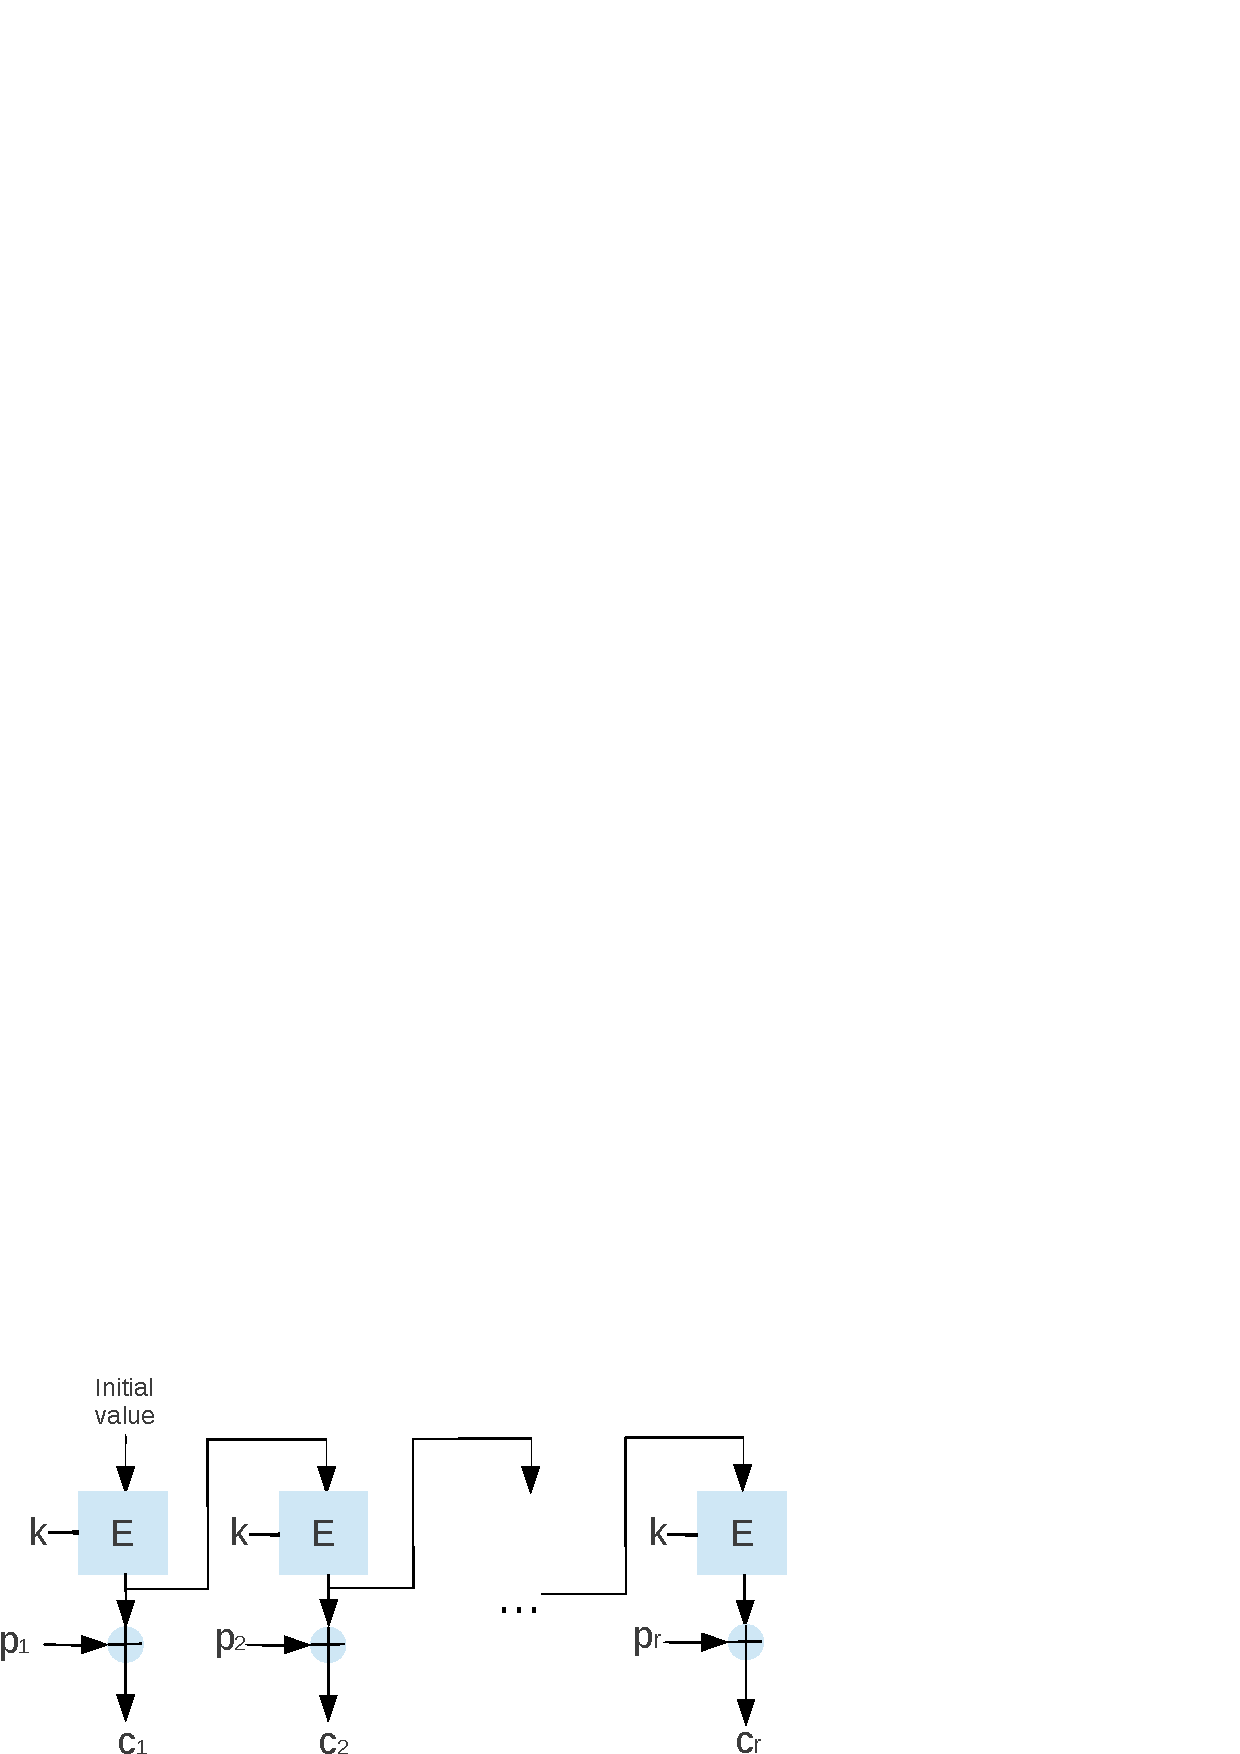
\includegraphics[scale=0.8]{Pictures/OFB_En.pdf} 
\caption{Workflow of the OFB encryption. Adapted from \cite{DBLP:reference/crypt/2011}.}\label{OFBEN}
\end{figure}
\subsubsection*{Decryption}
Mathematical description : $P_i=C_i\oplus K_i\,,\, K_i=E_K(K_{i-1})$.\\
The algorithm encryption is used in decryption as shown in Figure \ref{OFBDE}. The keystream block $K_0$ is initialized with the start value $IV$ or reinitialized by \texttt{Set\_IV()}. $K_{i-1}$ will be encrypted to $K_i$ and XORed with $C_i$. The result of the operation is the plaintext block $P_i$. These ciphertext blocks are decrypted in the same sequence in which they are generated.
\begin{figure}[h]
\centering
\includegraphics[scale=0.8]{Pictures/OFB_De.pdf} 
\caption{Workflow of the OFB decryption. Adapted from \cite{DBLP:reference/crypt/2011}.}\label{OFBDE}
\end{figure}
\subsubsection*{Remarks}
With the "Low-Level-API" (\ref{Low-Level-OFB}) users can generate a keystream without plaintext blocks. Thereby they can encrypt the plaintext blocks very fast. For example it will be possible to generate keystream blocks at night and then encrypt plaintext blocks in the day time. So this mode is very suitable when phasic plaintext blocks should be encrypted quickly.
\subsubsection*{Notice:}
\begin{itemize}
\item The keystream repeats at any time. That is, $\exists L:K_0=K_L$. Supposed $m$ is the block size in bits, then the average length of a cycle goes to $2^m-1$ bits.
\item A bit error in plaintext will influence one bit in ciphertext and vice versa.
\item Manipulation on plaintext is clear, every change in ciphertext influences directly the plaintext.
\item Error in synchronization (Alice and Bob are in different counter states) can not be solved. 
\end{itemize}
\subsubsection*{Low-Level-API}\label{Low-Level-OFB}
The following API can be used only when you know what it does.
\begin{lstlisting}{}
  procedure Next_Block(Keystream : out Block);
\end{lstlisting}
Mathematical description : $K_i=E_K(K_{i-1})$.\\
During initialization the start value IV is stored as keystream block $K_0$. Every time when the \texttt{Next\_Block()} procedure is called, the keystream block $K_i$ will be encrypted to $K_{i+1}$ and resulted as keystream.
%%%%%%%%%%%%%%%%%%%%%%%%%%%%%%%%%%%%%%%%%%%%%%%%%%%%%%%%%%%
%%%%%%%%%%%%%%%%%%%%%%%%%%%%%%%%%%%%%%%%%%%%%%%%%%%%%%%%%%%
\section{Example}
\subsubsection*{CBC Mode}
\begin{lstlisting}{}
  with Crypto.Types;
  with Ada.Text_IO;
  with Crypto.Symmetric.Blockcipher_Tripledes;
  with Crypto.Symmetric.Mode.CBC;
  procedure Example_CBC_Mode is
	 use Ada.Text_IO; use Crypto.Types;
    package TDES renames Crypto.Symmetric.Blockcipher_Tripledes;
    -- use TDES in secure CBC mode
    package TDES_CBC is new Crypto.Symmetric.Mode.CBC(TDES);
	 use TDES_CBC;
    Key: B_Block192 := (16#00#, 16#00#, 16#00#, 16#00#, 16#00#, 
                        16#00#, 16#00#, 16#00#, 16#00#, 16#00#, 
                        16#00#, 16#00#, 16#00#, 16#00#, 16#00#, 
                        16#00#, 16#01#, 16#23#, 16#45#, 16#67#, 
                        16#89#, 16#ab#, 16#cd#, 16#ef#);
    IV: B_Block64 := (16#12#, 16#34#, 16#56#, 16#78#,
            	          16#90#, 16#ab#, 16#cd#, 16#ef#);
    --Plaintext
    P_String: String :="Now is the time for all.";
    --Plaintext will be divided in 3*64 bit blocks.
    P: array(1..3) of B_Block64 := 
			(To_B_Block64(To_Bytes(P_String(1..8))),
          To_B_Block64(To_Bytes(P_String(9..16))),
			 To_B_Block64(To_Bytes(P_String(17..24))));
    --Ciphertext
    C: array(0..3) of B_Block64;
    begin
      Init(Key, IV);    --1. Initialization
      C(0):= IV;        --1. Ciphertext block = start value
      for I in P'Range loop
	     Encrypt(P(I),C(I));  --Encryption
      end loop;
      --For decryption the start value will be 
      --reinitialized with the same value.
      Set_IV(C(0));         
      for I in P'Range loop
         Decrypt(C(I),P(I));   --Decryption
         Put(To_String(To_Bytes(P(I))));
      end loop;
  end Example_CBC_Mode;
\end{lstlisting}\\ \ \\
\subsubsection*{BPS Mode}
\begin{lstlisting}{}
  with Crypto.Symmetric.Mode.BPS;
  with Crypto.Symmetric.Blockcipher_AES128;
  with Crypto.Types; use Crypto.Types;
  with Ada.Text_IO; use Ada.Text_IO;
  procedure Example_BPS_Mode is
    package AES128 renames Crypto.Symmetric.Blockcipher_AES128;
    package BPS is new Crypto.Symmetric.Mode.BPS(AES128);
    use BPS;
    Key : B_Block128 := (16#12#, 16#34#, 16#56#, 16#78#,
	  	                 16#90#, 16#ab#, 16#cd#, 16#ef#,
		                 16#12#, 16#34#, 16#56#, 16#78#,
		                 16#90#, 16#ab#, 16#cd#, 16#ef#);
    IV : B_Block64 :=(16#12#, 16#34#, 16#56#, 16#78#,
		                16#90#, 16#ab#, 16#cd#, 16#ef#);
    Plaintext : BPS.Numerals(1..10) := (0,1,2,3,4,5,6,7,8,9);
    Ciphertext, P : BPS.Numerals(1..10);
    Result : Boolean := False;
  begin
    Init(Key, IV);
    Encrypt(Plaintext, Ciphertext);
    Decrypt(Ciphertext, P);
    for I in Plaintext'Range loop
       if Plaintext(I) = P(I) then
          Result := True;
       end if;
    end loop;
    if Result then
       Put_Line("OK");
    else
       Put_Line("Error"); 
    end if;
  end Example_BPS_Mode;
\end{lstlisting}
\chapter{Crypto.Symmetric.Mode.Oneway}
This generic package works with one-way blockciphers in one-way modes. It integrates a one-way block cipher with a feedback and also some easy operations ($+,xor$). A one-way mode will be initialized with a random start value (Initial Value (IV)). The ciphertext is therefore not only dependent on the used mode, plaintext and key, but also on the random start value. When users encrypt a plaintext twice with the same key in the same mode but different IVs, then they will get different ciphertexts, i.e. a oneway mode encrypts two plaintext blocks $P_1$ and $P_2$ with $P_1=P_2$ to two ciphertext blocks $C_1$ and $C_2$ with overwhelming probability that $C_1\neq C_2$. So that it is now possible to encrypt more messages with the same key.\\
\textbf{Notice: To decrypt a ciphertext the key and start value by encryption are required.} For this reason the start value should be always kept together with the related ciphertext. \textbf{The security of a mode is independent from the familarity of the start value.} Hense, man multiplies usually the start value with the ciphertext as the final output by attaching the ciphertext to the start value ($C'=IV||C$).
%%%%%%%%%%%%%%%%%%%%%%%%%%%%%%%%%%%%%%%%%%%%%%%%%%%%%%%%%%%%%%
%%%%%%%%%%%%%%%%%%%%%%%%%%%%%%%%%%%%%%%%%%%%%%%%%%%%%%%%%%%%%%
\subsubsection*{Remarks}
\begin{itemize}
\item In a oneway mode it goes similarly as in a normal mode. If a normal mode can be used also as a oneway mode, then you should still prefer oneway mode, because it's nimbler.  
\item The API of this package is the same as in normal modes (\ref{API-Mode}).
\item Supported oneway modes:
\begin{itemize}
\item Cipher Feedback Mode (CFB) (\ref{CipherFeedbackMode})
\item Counter Mode (CTR) (\ref{CounterMode})
\item Output Feedback Mode (OFB) (\ref{OutputFeedbackMode})
\end{itemize}
\end{itemize}
\subsubsection*{Example}
\begin{lstlisting}{}
  with Crypto.Types;
  with Ada.Text_IO;
  with Crypto.Symmetric.Oneway_Blockcipher_Twofish128;
  with Crypto.Symmetric.Mode.Oneway_CTR;
  procedure Example_Mode_Oneway is
	 use Ada.Text_IO; use Crypto.Types;
    package TF128 renames 
                  Crypto.Symmetric.Oneway_Blockcipher_Twofish128;
    package Twofish128 is new
                  Crypto.Symmetric.Mode.Oneway_CTR(TF128);
 	 use Twofish128;
    Key: B_Block128 := (16#2b#, 16#7e#, 16#15#, 16#16#, 16#28#,
                        16#ae#, 16#d2#, 16#a6#, 16#ab#, 16#f7#,
                        16#15#, 16#88#, 16#09#, 16#cf#, 16#4f#,
                        16#3c#);
    IV: B_Block128 := (15 => 1, others => 0);
     --Plaintext
    P_String: String :="All your base are belong to us! ";
     --Plaintext will be divided in 2*64 bit blocks.
    P: array(1..2) of B_Block128 := 
			(To_B_Block128(To_Bytes(P_String(1..16))),
			 To_B_Block128(To_Bytes(P_String(17..32))));
    C: array(0..2) of B_Block128;      --Ciphertext
  begin
    Init(Key, IV);         --Initialization
    C(0):= IV;             --1. Ciphertext block = start value
    for I in P'Range loop
	    Encrypt(P(I),C(I));   --Encryption
    end loop;
     --For decryption the start value will be reinitialized.
    Set_IV(C(0));
    for I in P'Range loop
	    Decrypt(C(I),P(I));     --Decryption
       Put(To_String(To_Bytes(P(I))));
    end loop;
  end Example_Mode_Oneway;
\end{lstlisting}
\chapter{Crypto.Symmetric.Hashfunction}\label{Hash}
In this generic package a cryptographic hash function is generated
from the algorithm of a cryptographic hash function (Chapter
\ref{AlgorithmHash}), which is used for the following purposes:
\begin{itemize}
\item Integrity testing of messages
\item Creation and verification of digital signatures
\item Creation of random numbers or random bits
\end{itemize}
The purpose of this package is to standardize and simplify the API for
hash functions.
\section{API}
\subsubsection*{Generic Part}
\begin{lstlisting}{}
  generic
   type Hash_Type                 is private;
   type Message_Type              is private;
   type Message_Block_Length_Type is range <>;
	 type Internal_Scheme		  is private;
	
   with function Generic_To_Bytes(DWord_Array : Hash_Type)
   								      return Bytes is <>;
												
   with procedure Init(This : in out Internal_Scheme) is <>;
   with procedure Round(This : in out Internal_Scheme;
                        Message_Block : in     Message_Type) is <>;
   with function Final_Round(This : in out Internal_Scheme;
                             Last_Message_Block  : Message_Type;
                             Last_Message_Length : Message_Block_Length_Type)
                            return Hash_Type is <>;
   with procedure Hash(Message    : in   Bytes;
                       Hash_Value : out  Hash_Type) is <>;
   with procedure Hash(Message    : in   String;
                       Hash_Value : out  Hash_Type) is <>;
   with procedure F_Hash(Filename   : in   String;
                         Hash_Value : out  Hash_Type) is <>;
\end{lstlisting}
The API of a generic hashfunction is made of a High- and a
Low-Level-API. The Low-Level-API should be only used when the user is
familiar with the cryptographic hashfunction. If it's not in this
situation, then please only use the High-Level-API.

\subsubsection*{High-Level-API}
\begin{lstlisting}{}
  function Hash  (Message  : Bytes)  return Hash_Type;
  function Hash  (Message  : String) return Hash_Type;
  function F_Hash(Filename : String) return Hash_Type;
\end{lstlisting}
The function \texttt{Hash()} returns a hash value of a message. The
type of the message can either be bytes or a string. The function
\texttt{F\_Hash()} works on a file. For example:
$H:=F\_Hash("/bin/ls")$; returns a hash value of "$/bin/ls$".

\subsubsection*{Low-Level-API}
The Low-Level-API consists of the following operations.
\begin{itemize}
\item One procedure \texttt{Initialize()} initializes or reinitializes the hash function. Every time before a message is to be hashed, this
  procedure should be called.
\begin{lstlisting}{}
  procedure Initialize(This : in out Hash_Context);
\end{lstlisting}
\item One procedure \texttt{Update()} can be called iteratively to hash
  message blocks.
\begin{lstlisting}{}
  procedure Update(This : in out Hash_Context;
                   Message_Block : in Message_Type);
\end{lstlisting}
\item Function \texttt{Final\_Round()} pads and hashs a message block
  \texttt{Last\_Message\_Block}. Because of padding, the length of the
  exact message content \texttt{Message\_Block\_Length\_Type} should
  be specified in byte. Usually a message is shorter than a message
  block of type \texttt{Message\_Type}. The returning value of the
  function is corresponding to the final hash value of the message.
\begin{lstlisting}{}
 function Final_Round(This : in out Hash_Context;
                      Last_Message_Block  : Message_Type;
                      Last_Message_Length : Message_Block_Length_Type)
                       return Hash_Type;
\end{lstlisting}
\end{itemize}

%%%%%%%%%%%%%%%%%%%%%%%%%%%%%%%%%%%%%%%%%%%%%%%%%%%%%%%%%%%
%%%%%%%%%%%%%%%%%%%%%%%%%%%%%%%%%%%%%%%%%%%%%%%%%%%%%%%%%%%

\section{Example}
\subsubsection*{High-Level-API}
This example gives the SHA-256 hash value of $/bin/ls$.
\begin{lstlisting}{}
  with Ada.Text_IO; use Ada.Text_IO;
  with Crypto.Types; use Crypto.Types;
  with Crypto.Symmetric.Hashfunction_SHA256;

  procedure Example_Hash_HL is
    package SHA256 renames
    							Crypto.Symmetric.Hashfunction_SHA256;
    Hash : W_Block256 := SHA256.F_Hash("/bin/ls");
  begin
    for I in Hash'Range loop
      Put(To_Hex(Hash(I)));
    end loop;
    Put_Line(" /bin/ls");
  end Example_Hash_HL;
\end{lstlisting}
\subsubsection*{Low-Level-API}
\begin{lstlisting}{}
  with Ada.Text_IO;   use Ada.Text_IO;
  with Crypto.Types;  use Crypto.Types;
  with Crypto.Symmetric.Hashfunction;
  with Crypto.Symmetric.Algorithm.SHA256;
  use Crypto.Symmetric.Algorithm.SHA256;
  pragma Elaborate_All(Crypto.Symmetric.Hashfunction);

  procedure Example_Hash_LL is
    package WIO is new Ada.Text_IO.Modular_IO(Word);
		package SHA256 is new Crypto.Symmetric.Hashfunction
								(Hash_Type                 => W_Block256,
                 Message_Type              => W_Block512,
                 Message_Block_Length_Type => 
								     Crypto.Types.Message_Block_Length512,
                 Internal_Scheme           => Sha256_Interface,
                 Generic_To_Bytes	     => Crypto.Types.To_Bytes);
    Message : String :=("All your base are belong to us! ");
    W : Words := To_Words(To_Bytes(Message));
    M : W_Block512 := (others => 0);
    H : W_Block256;
		H_Context : SHA256.Hash_Context;
  begin
    for I in W'Range loop
      M(I) := W(I);
    end loop;
    H_Context.Initialize;
    H := H_Context.Final_Round(M, Message'Last);
    for I in W_Block256'Range loop
      WIO.Put(H(I), Base=>16);
      New_Line;
    end loop;
    New_Line;
  end Example_Hash_LL;
\end{lstlisting}
\subsection*{Remark:}
Users don't need to generate every time a new hash function. There are
already hash functions defined in the ACL.
\begin{itemize}
\item \texttt{Crypto.Symmetric.Hashfunction\_SHA1}
\item \texttt{Crypto.Symmetric.Hashfunction\_SHA256}
\item \texttt{Crypto.Symmetric.Hashfunction\_SHA512}
\item \texttt{Crypto.Symmetric.Hashfunction\_Whirlpool}
\end{itemize}

\chapter{Crypto.Symmetric.MAC}\label{MAC}
A message authentication code (MAC) ensures the integrity of a message and sender authentication. It uses a symmetric key (RMAC uses two symmetric keys). The result of the MAC is named an authentication tag. The developer of this library marks it as a (digital) stamp. Three MACs are provided in the ACL, they are randomized MAC (RMAC), hash function based MAC (HMAC) and cipher-based MAC (CMAC).
\section{Randomized MAC (RMAC)}
RMAC is developed by Eliane Jaulmes, Antoine Joux and Frederic Valette. It is based on CBC-MAC and one-way block cipher (Chapter \ref{Oneway-Blockcipher}). It is proved save against the birthday attack. Two keys are required in RMAC.\\
Mathematical description: $RMAC_{K_1,K_2}(E,M)=E_{K_2\oplus R}(C_n)$\,, with $C_i=E_{K_1}(M_i\oplus C_{i-1})$, $R\in_R\{0,1\}^{|K_1|}$ and $C_0=0^n$.
\subsubsection*{Generic Part}
\begin{lstlisting}{}
  generic
    with package C is new 
    					Crypto.Symmetric.Oneway_Blockcipher(<>);
    with procedure Read (Random : out C.Key_Type) is <>;
    with function "xor" (Left, Right : C.Block) return C.Block is <>;
    with function "xor" (Left, Right : C.Key_type) 
     							return C.Key_Type is <>;
\end{lstlisting}
\newpage
\subsubsection*{High-Level-API}
\begin{lstlisting}{}
  type Blocks  is array (Integer range <>) of Block;
  procedure Sign(Message    : in Blocks;
                 Key1, Key2 : in Key_Type;
                 R          : out Key_Type;
                 Tag        : out Block);
  function Verify(Message    : in Blocks;
                  Key1, Key2 : in Key_Type;
                  R          : in Key_Type;
                  Tag        : in Block)  return Boolean;
\end{lstlisting}\\
The procedure \texttt{Sign()} signs \texttt{Message} with two keys, Key1 and Key2. The message is delivered as an array of blocks. Key1 is used to encrypt the whole message blocks, and Key2 is used to generate the final tag based on the calculated ciphertext.
The function \texttt{Verify()} returns true if the term \texttt{Tag} is a valid stamp, otherwise it returns false. When one or more parameters don't agree with those generated from the procedure \texttt{Sign()}, then the function returns false with a significant probability.\\
\subsubsection*{Low-Level-API}
\begin{lstlisting}{}
  procedure Init(Key1, Key2    : in Key_Type);
  procedure Sign(Message_Block : in Block);
  procedure Final_Sign(Final_Message_Block : in Block;
                       R    : out Key_Type;
                       Tag  : out Block);
  procedure Verify(Message_Block : in Block);
  function Final_Verify(Final_Message_Block : in Block;
                        R   : in Key_Type;
                        Tag : in Block)   return Boolean;
\end{lstlisting}
\begin{itemize}
\item The procedure \texttt{Init()} initializes RMAC with two keys, and sets an internal initial state.
\item The procedure \texttt{Sign()} encrypts a message block (\texttt{Message\_Block}). Every time it works only on one block, if there are blocks more than one, the procedure should be called til the last block.
\item The procedure \texttt{Final\_Sign()} encrypts the last message block \texttt{Final\_Message\_Block}, and then generates a random number $R$ to calculates the stamp $Tag$, and finally resets RMAC.
\item The procedure \texttt{Verify()} encrypts a message block (\texttt{Message\_Block}). Every time it works only on one block.
\item The function \texttt{Final\_Verify()} decrypts the last message block \texttt{Final\_Message\_Block}, calculates a new tag and then compares the tag with the delivered one to test if it is valid. True is returned if valid, otherwise false.
\end{itemize}
\subsubsection*{Example}
\begin{lstlisting}{}
  with Crypto.Types; use Crypto.Types;
  with Ada.Text_IO; use Ada.Text_IO;
  with Crypto.Types.Random; use Crypto.Types.Random;
  with Crypto.Symmetric.MAC.RMAC;
  with Crypto.Symmetric.Oneway_Blockcipher_AES128;
  pragma Elaborate_All(Crypto.Symmetric.MAC.RMAC);
  procedure Example_RMAC is
   package AES128 renames Crypto.Symmetric.Oneway_Blockcipher_AES128;
    package RMAC128 is new Crypto.Symmetric.MAC.RMAC(AES128);
    use RMAC128;
    Key1: B_Block128:= (16#00#, 16#01#, 16#02#, 16#03#, 16#04#,
                        16#05#, 16#06#, 16#07#, 16#08#, 16#09#,
                        16#0a#, 16#0b#, 16#0c#, 16#0d#, 16#0e#, 
                        16#0f#);
    Key2 : B_Block128:=(16#00#, 16#11#, 16#22#, 16#33#, 16#44#,
                        16#55#, 16#66#, 16#77#, 16#88#, 16#99#,
                        16#aa#, 16#bb#, 16#cc#, 16#dd#, 16#ee#, 
                        16#ff#);
    R, Tag : B_Block128;
    M : String :="All your base are belong to us! ";
    Message : RMAC128.Blocks(0..1) := 
                        (To_B_Block128(To_Bytes(M(1..16))),		
                         To_B_Block128(To_Bytes(M(17..32))));
  begin
     -- Low-Level
    Init(Key1, Key2);
  	 Sign(Message(0));
  	 Final_Sign(Message(1), R, Tag);
 	 Init(Key1, Key2);
  	 Verify(Message(0));
  	 Put_Line(Final_Verify(Message(1), R, Tag)'Img);
  end Example_RMAC;
\end{lstlisting}
\section{Hash-based MAC (HMAC)}
The designers of HMAC are Mihir Bellare, Ran Canettiy and Hugo Krawczykz. It is based on a hash function. In addition, HMAC\_SHA1, HMAC\_SHA256, HMAC\_512 and HMAC\_Whir\-lpool are available.\\
Mathematical description: $HMAC_K(H,M)=H(K\oplus opad,H((K\oplus ipad)||M))$\,, with $opad=\{0x5C\}^n$ and $ipad=\{0x36\}^n$.
\subsubsection*{Generic Part}
\begin{lstlisting}{}
  generic
    with package H is new Crypto.Symmetric.Hashfunction(<>);
    with function "xor"(Left, Right : H.Message_Type) 
      					          return H.Message_Type is <>;
    with procedure Fill36 (Ipad : out  H.Message_Type) is <>;
    with procedure Fill5C (Opad : out  H.Message_Type) is <>;
    with procedure Copy (Source : in  H.Hash_Type; 
      					    Dest   : out H.Message_Type) is <>;
\end{lstlisting}

The two procedures \texttt{Fill36()} and \texttt{Fill5C()} make the outer/inner padding with value $0x36$ or $0x5C$.
The procedure \texttt{Copy()} copies the content of \texttt{Source} to \texttt{Dest}. If the size of the source value is smaller than that of the destination value, then the rest will be padded with zeros.
All these helping operations are defined in \texttt{Crypto.Symmetric.MAC}.\\
\subsubsection*{API}
\begin{lstlisting}{}
  procedure Init(Key : in Message_Type);
  procedure Sign(Message_Block : in Message_Type);
  procedure Final_Sign
      (Final_Message_Block        : in Message_Type;
       Final_Message_Block_Length : in Message_Block_Length_Type;
       Tag                        : out Hash_Type);
  procedure Verify(Message_Block : in Message_Type);
  function Final_Verify
      (Final_Message_Block        : Message_Type;
       Final_Message_Block_Length : Message_Block_Length_Type;
       Tag                        : Hash_Type) return Boolean;
\end{lstlisting}
\begin{itemize}
\item Procedure \texttt{Init()} initializes the \texttt{HMAC} with the key and sets an initial state.
\item Procedure \texttt{Sign()} hashs a message block (\texttt{Message\_Block}). It is called until to the second to last block.
\item Procedure \texttt{Final\_Sign()} hashs the last message block of the length \texttt{Final\_Message\_B\-lock\_Length}, returns a digital stamp tag and resets the HMAC.
\item Procedure \texttt{Verify()} hashs a message block.
\item The function \texttt{Final\_Verify()} hashs the last message block of the length \texttt{Final\_Message\_B\-lock\_Length}, then verifies whether the tag is valid or not. It returns true if valid, else false.
\end{itemize}
\subsubsection*{Example}
\begin{lstlisting}{}
  with Crypto.Types;
  with Ada.Text_IO;
  with Crypto.Symmetric.MAC;
  with Crypto.Symmetric.MAC.HMAC;
  with Crypto.Symmetric.Hashfunction_SHA256;
  use Crypto.Types;
  use Ada.Text_IO;
  pragma Elaborate_All(Crypto.Symmetric.MAC.HMAC);
  procedure Example_HMAC is
    package HMAC256 is new Crypto.Symmetric.MAC.HMAC
				      (H =>Crypto.Symmetric.Hashfunction_SHA256,
		    		 	 Copy =>Crypto.Symmetric.MAC.Copy,
						 Fill36 =>Crypto.Symmetric.MAC.Fill36,
						 Fill5C =>Crypto.Symmetric.MAC.Fill5C);
    use HMAC256;
    Key : W_Block512 :=(0 => 16#0b0b0b0b#, 1 => 16#0b0b0b0b#,
		                  2 => 16#0b0b0b0b#, 3 => 16#0b0b0b0b#,
		                  4 => 16#0b0b0b0b#, others => 0);
    Message : W_Block512 :=(0 => 16#48692054#, 
    								 1 => 16#68657265#, others => 0);
    Tag : W_Block256;
  begin
    Init(Key);
    Final_Sign(Message, 8, Tag);
    Put_Line(Final_Verify(Message, 8, Tag)'Img);
  end Example_HMAC;
\end{lstlisting}
\subsection*{Remark:}
The users don't need to generate a new HMAC every time. There are already HMACs defined in the ACL.
\begin{itemize}
\item \texttt{Crypto.Symmetric.Mac.Hmac\_SHA1}
\item \texttt{Crypto.Symmetric.Mac.Hmac\_SHA256}
\item \texttt{Crypto.Symmetric.Mac.Hmac\_SHA512}
\item \texttt{Crypto.Symmetric.Mac.Hmac\_Whirlpool}
\end{itemize}
\section{Cipher-based MAC (CMAC)}
CMAC is a blockcipher-based message authentication code. It is used to assure authenticity and integrity of the data.
CMAC is a OMAC1 described in \cite{DBLP:conf/fse/2003}. As shown in Figure \ref{OMAC}, the message is devided into blocks $m_1,m_2,\cdots,m_r$\,, and the first $r-1$ blocks will be processed in a signature algorithm iteratively. The intermediate values are $t_1,t_2,\cdots, t_{r-1}$. Each round can be described mathematically as:
\begin{equation*}
t_i=E_k(t_{i-1}\oplus m_i), \quad 1\leq i \leq r-1\,,\,\mbox{and $t_0$ is a zero block}\,.
\end{equation*}
For the last message block, if it is a full block, then:
\begin{equation*}
Tag=E_k(t_{r-1}\oplus m_r \oplus U)\,,
\end{equation*}
if the block is not a full block, then it will be padded with a one bit and zero bits until it is full, and then:
\begin{equation*}
Tag=E_k(t_{r-1}\oplus m_r \oplus U_2)\,.
\end{equation*}
The terms $U$ and $U_2$ are two non-zero constants based on $L$ in the Galois
field $GF(2^n)$, where $L=E_k(0^n)$. A function is used to calculate $U$ from $L$, and $U_2$ from $U$. It is satisfied that $U\neq U_2$, otherwise, for a full block $m=m'10^*$ and a not full block $m'$, after padding the second block becomes $m'10^*$, they will lead to two identical tags, which is against our design purpose.
Details about this function can be found in \cite{DBLP:conf/fse/2003}.
\begin{figure}[h]
\centering
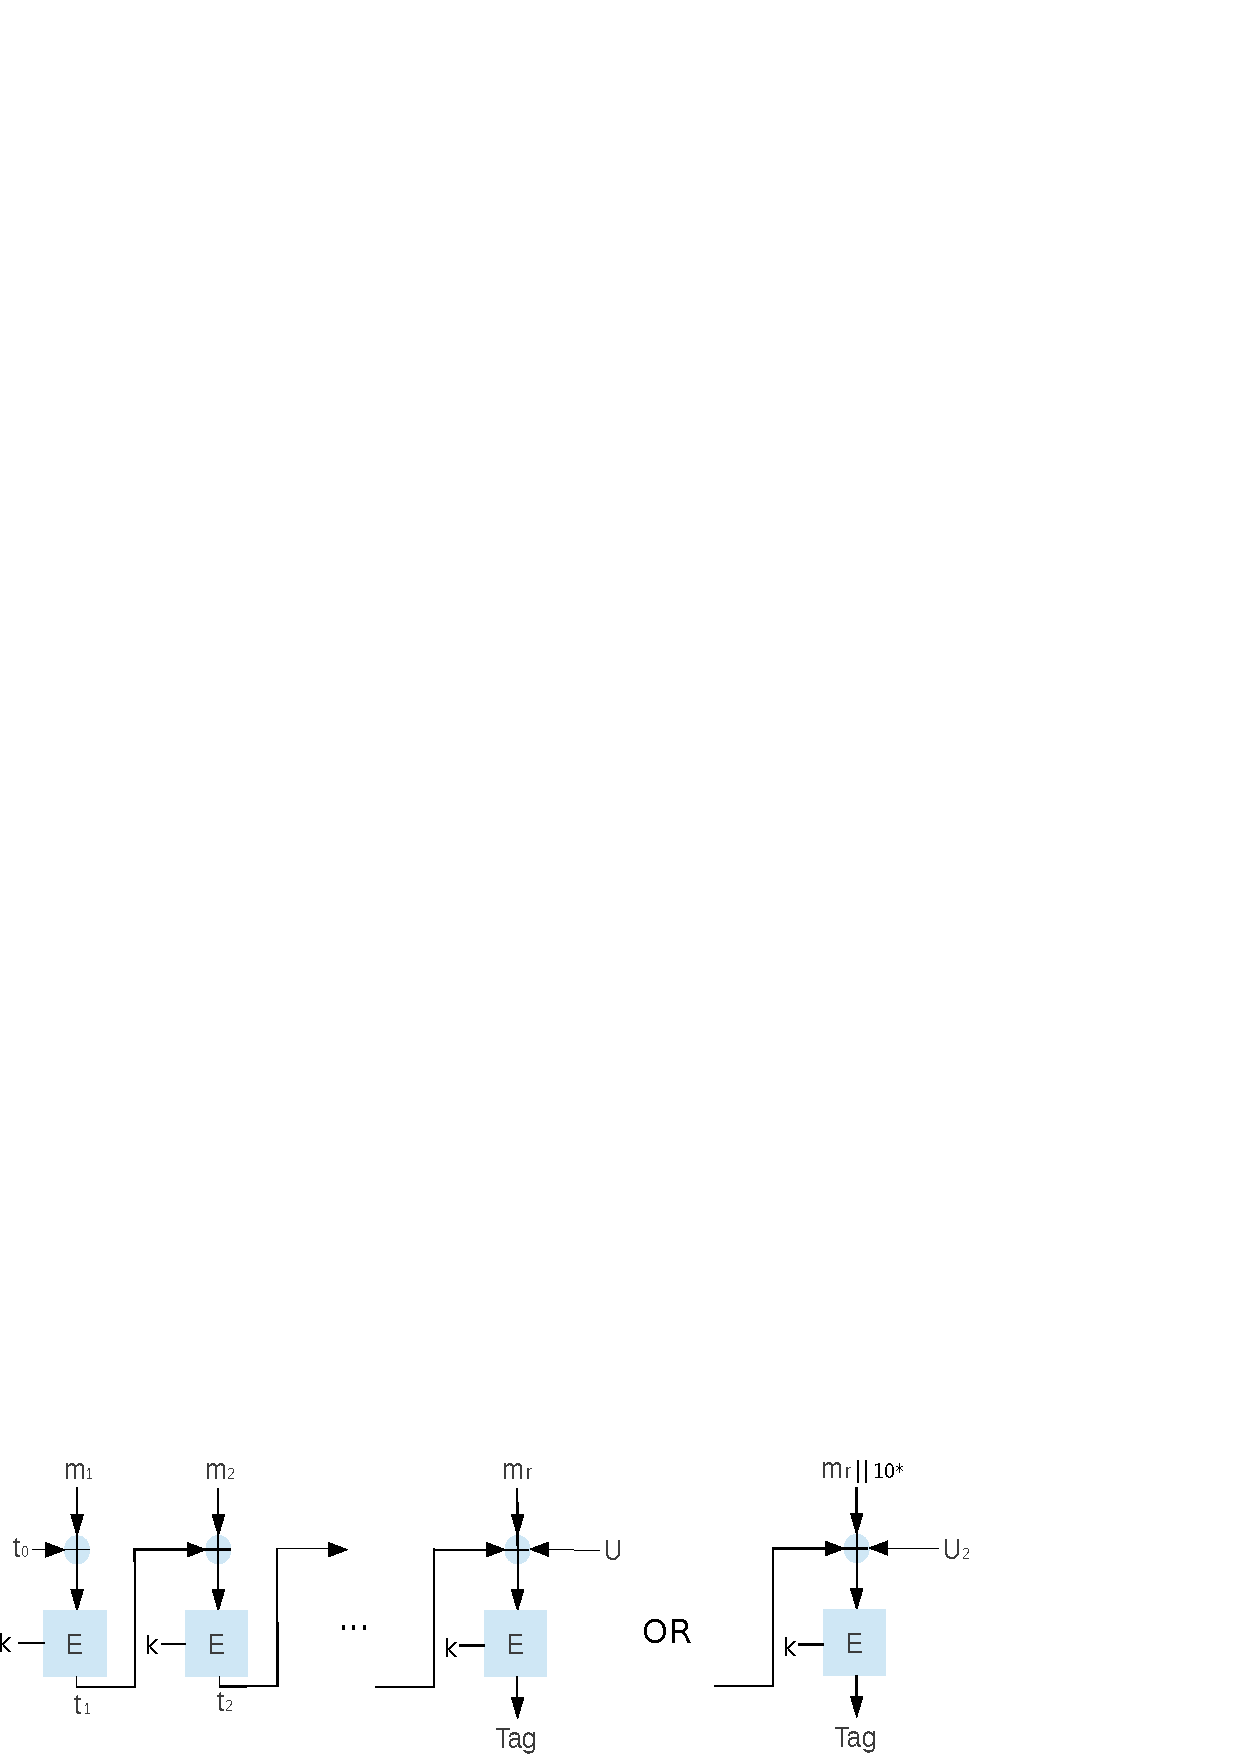
\includegraphics[scale=0.8]{Pictures/CMAC.pdf} 
\caption{The workflow of the CMAC.}\label{OMAC}
\end{figure}
\newpage
\subsubsection*{Generic Part}
\begin{lstlisting}{}
  generic
   with package C is new 
   					Crypto.Symmetric.Oneway_Blockcipher(<>);
   with function To_Block_Type (B : Bytes) return C.Block;
   with function To_Bytes (B : C.Block) return Bytes;
   with function Shift_Left (Value : C.Block; 
   								  Amount: Natural) return C.Block;
   with function "xor" (Left, Right : C.Block) return C.Block is <>;
\end{lstlisting}
\subsubsection*{High-Level-API}
\begin{lstlisting}{}
  type Blocks is array (Integer range <>) of Block;
  procedure Sign(Message : in  Blocks;
                 Key     : in  Key_Type;
                 Tag     : out Block);
  function Verify(Message : in Blocks;
                  Key     : in Key_Type;
                  Tag     : in Block) return Boolean;
\end{lstlisting}
Procedures and functions of high-level use the functions in low-level. Users should always use the high-level interfaces. The message is signed block by block calling internally low-level functions. The function \texttt{Verify()} returns true if the newly created tag equals the delivered tag, else false is returned.\\
\textbf{Exception:} The terms $U$ and $U_2$ (as marked in Figure \ref{OMAC}) are designed in 8 bytes or 16 bytes, which depends on the block size. If the block size is neither 64 bits nor 128 bits:\quad\texttt{Blocklength\_Not\_Supported}.\\
\subsubsection*{Low-Level-API}
\begin{lstlisting}{}
  procedure Init(Key : in Key_Type);
  procedure Sign(Message_Block : in Block);
  procedure Final_Sign(Final_Message_Block : in  Block;
                       Bytes_Read          : in  Natural;
                       Tag                 : out Block);
  procedure Verify(Message_Block : in Block);
  function Final_Verify(Final_Message_Block : in Block;
                        Bytes_Read          : in Natural;
                        Tag                 : in Block)
                        return Boolean;
\end{lstlisting}
\begin{itemize}
\item Procedure \texttt{Init()} makes initialization of the CMAC.
\item Procedure \texttt{Sign()} encrypts one message block (\texttt{Message\_Block}).
\item Procedure \texttt{Final\_Sign()} encrypts the last message block \texttt{Final\_Message\_Block}. If \texttt{Bytes\_Read} of the last message block isn't equal $Block'Size/8$, then it makes padding. A tag is generated and the CMAC is reset.
\item Procedure \texttt{Verify()} encrypts a message block. The block is processed as in procedure \texttt{Sign()}.
\item Procedure \texttt{Final\_Verify()} encrypts the last message block, and makes comparison of a newly generated tag with the delivered tag. It returns true if the two tags are equal, else false.
\end{itemize}
\subsection*{Example}
\begin{lstlisting}{}
  with Ada.Text_IO; use Ada.Text_IO;
  with Crypto.Types; use Crypto.Types;
  with Crypto.Symmetric.Oneway_Blockcipher_AES128;
  with Crypto.Symmetric.MAC.CMAC;
  pragma Elaborate_All(Crypto.Symmetric.MAC.CMAC);

  procedure Example_CMAC is
   package AES128 renames Crypto.Symmetric.Oneway_Blockcipher_AES128;
    package CMAC128 is new Crypto.Symmetric.MAC.CMAC(
						C => AES128, To_Block_Type => To_B_Block128,
						To_Bytes => To_Bytes, 
						Shift_Left => Shift_Block_Left, 
						"xor" => "xor");
    use CMAC128;
    Key : B_Block128 := 
             (16#2b#, 16#7e#, 16#15#, 16#16#, 16#28#, 16#ae#,
		       16#d2#, 16#a6#, 16#ab#, 16#f7#, 16#15#, 16#88#,
		       16#09#, 16#cf#, 16#4f#, 16#3c#);
    Message: CMAC128.Blocks(1..1) :=  (1=>(others=>0));
    Tag : B_Block128;
    Tag_New : B_Block128 := 
        (16#bb#, 16#1d#, 16#69#, 16#29#, 16#e9#, 16#59#,
			16#37#, 16#28#, 16#7f#, 16#a3#, 16#7d#, 16#12#,
			16#9b#, 16#75#, 16#67#, 16#46#);
  begin
    Sign(Message, Key, Tag);
    Put_Line(Verify(Message, Key, Tag_New)'Img);
  end Example_CMAC;
\end{lstlisting}


\chapter{Crypto.Symmetric.AE}\label{AE}
Authenticated encryption (AE) schemes are symmetric-key mechanisms by
which a message M is transformed in to a ciphertext C in such a way
that C protects both privacy and authenticity
\cite{DBLP:journals/iacr/BellareRW03}. This package is specified in
\texttt{Crypto.Symmetric.AE}.
\subsubsection*{Generic Part}
\begin{lstlisting}{}
  generic
    type Key_Type is private;
    type Block is private;
    with package N is new Crypto.Types.Nonces(Block);
\end{lstlisting}
\subsubsection*{Types}
\begin{lstlisting}{}
  type AE_Scheme is limited interface;
  type Callback_Writer is access procedure (B : in  Bytes);
  type Callback_Reader is access procedure
  									(B : out Bytes; Count: out Natural);
\end{lstlisting}
In Ada \textbf{access} is like pointer in C++. Objects of an access
type, as the name implies, provide access to other objects and these
other objects can be allocated in a storage pool independent of the
block structure.

\subsubsection*{Procedures}
\begin{lstlisting}{}
  procedure Init_Encrypt(This   : out    AE_Scheme;
                         Key    : in     Key_Type;
                         Nonce  : in out N.Nonce'Class) is abstract;
  procedure Init_Decrypt(This        : out AE_Scheme;
                         Key         : in  Key_Type;
                         Nonce_Value : in  Block) is abstract;
  procedure Encrypt(This             : in out AE_Scheme;
                    Read_Plaintext   : in     Callback_Reader;
                    Write_Ciphertext : in     Callback_Writer) 
                    is abstract;
  function Decrypt_And_Verify
  					(This                   : in out AE_Scheme;
                Read_Ciphertext        : in Callback_Reader;
                Read_Ciphertext_Again  : in Callback_Reader := null;
                Write_Plaintext        : in Callback_Writer)
                return Boolean is abstract;
\end{lstlisting}
Notice that they are all abstract, they can not be called.

%%%%%%%%%%%%%%%%%%%%%%%%%%%%%%%%%%%%%%%%%%%%%%%%%%%%%%%%%%%%%%%%%%%%%
%%%%%%%%%%%%%%%%%%%%%%%%%%%%%%%%%%%%%%%%%%%%%%%%%%%%%%%%%%%%%%%%%%%%%

\section{AE.AD}
Authenticated Encryption with associated data (AEAD) is an extension
of the notion of authenticated encryption. The data has two fields, a
header ($H$) and a plaintext ($M$). The header $H$ consists of the
initial value/nonce $IV$. We denote an authenticated encryption scheme
with the requirement that the initial vector $IV$ is only used once in
a nonce based scheme. Otherwise, we call such a scheme deterministic
\cite{DBLP:conf/fse/FleischmannFL12}.
\subsubsection*{Types}
\begin{lstlisting}{}
  type AEAD_Scheme is limited interface;
\end{lstlisting}
\subsubsection*{Procedures}
\begin{lstlisting}{}
  procedure Encrypt(This            : in out AEAD_Scheme;
                    Read_Header     : in Callback_Reader;
                    Read_Plaintext  : in Callback_Reader;
                    Write_Ciphertext: in Callback_Writer)is abstract;
  function Decrypt_And_Verify
  				(This                   : in out AEAD_Scheme;
             Read_Header            : in     Callback_Reader;
             Read_Ciphertext        : in     Callback_Reader;
             Read_Ciphertext_Again  : in     Callback_Reader := null;
             Write_Plaintext        : in     Callback_Writer)
             return Boolean is abstract;
\end{lstlisting}
Notice that they are all abstract, they can not be called.\\

%%%%%%%%%%%%%%%%%%%%%%%%%%%%%%%%%%%%%%%%%%%%%%%%%%%%%%%%%%%%%%%%%%%%%
%%%%%%%%%%%%%%%%%%%%%%%%%%%%%%%%%%%%%%%%%%%%%%%%%%%%%%%%%%%%%%%%%%%%%

\section{AE\_OCB}
OCB stands for "Offset Codebook", which is fully parallelizable and
adds minor overhead. Desirable properties of OCB include the ability
to encrypt a string of arbitrary length, and no requirement for a
random IV \cite{DBLP:journals/tissec/RogawayBB03}. The OCB in the ACL
is defined as OCB3 by Ted Krovetz and Phillip Rogaway in
\cite{DBLP:conf/fse/KrovetzR11}. It shall be referred to as OCB
throughout this document.

\begin{figure}[h]
\centering
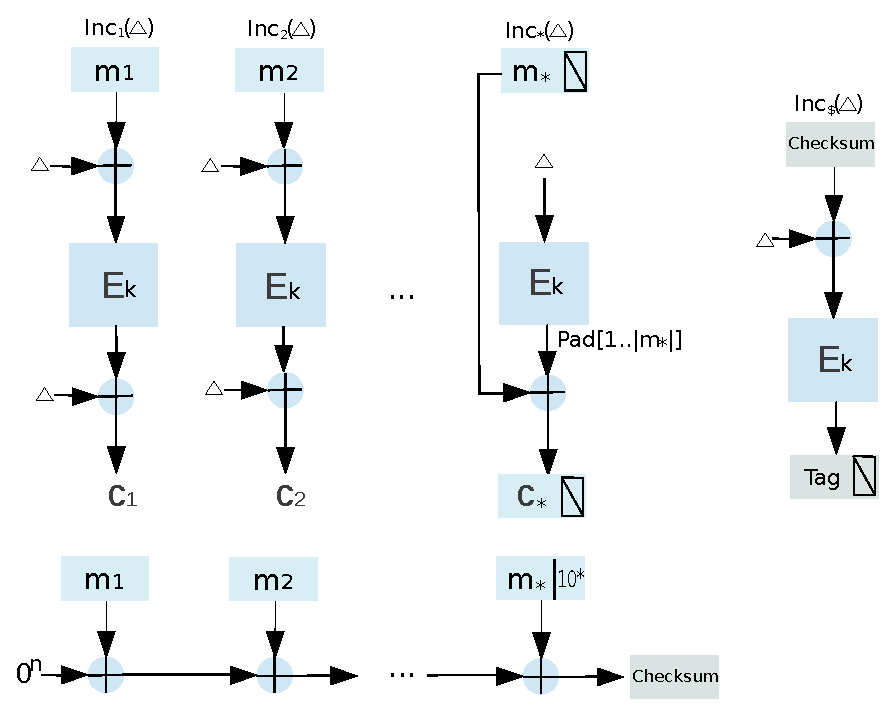
\includegraphics[scale=0.8]{./images/AE_OCB_En}
\caption{Workflow of the OCB encryption. Adapted from \cite{DBLP:conf/fse/KrovetzR11}.}\label{Workflow_OCB}
\end{figure}
Figure \ref{Workflow_OCB} shows the encryption of
AE\_OCB. \textbf{TOP} illustrates the situation of message M in a full
final block ($|M_4|=n$)(Checksum = $M_1\oplus M_2\oplus M_3\oplus
M_4$). \textbf{Bottom} is the situation that M has a short final
block, $1\leq |M_*|< n$,(Checksum = $M_1\oplus M_2\oplus M_3\oplus
M_*10^*$).

\subsubsection*{Generic Part}
\begin{lstlisting}{}
  generic
    with package BC is new Crypto.Symmetric.Blockcipher(<>);
    with package N is new Crypto.Types.Nonces(BC.Block);
    with function "xor" (Left, Right : in BC.Block)
    										return BC.Block is <>;
    with function To_Block_Type (B : Bytes) return BC.Block;
    with function To_Bytes (B : BC.Block) return Bytes;
    with function Shift_Left (Value: BC.Block; Amount: Natural)
    										return BC.Block;
    with function Shift_Right(Value: BC.Block; Amount: Natural)
    										return BC.Block;
    with function To_Byte_Word (X: Word) return Byte_Word;
\end{lstlisting}
The function \texttt{Shift\_Left()} is used to generate irreducible
polynomials $L(1..31)$. The function \texttt{Shift\_Right()} is used
to generate irreducible polynomial $L(-1)$.

\subsubsection*{Types}
\begin{lstlisting}{}
  type AE_OCB is new AE.AE_Scheme with private;
  Bytes_Per_Block : constant Positive := Block'Size / 8;
\end{lstlisting}
\subsubsection*{Procedures}
\begin{lstlisting}{}
  overriding
  procedure Init_Encrypt(This   : out    AE_OCB;
                         Key    : in     Key_Type;
                         Nonce  : in out N.Nonce'Class);
  overriding
  procedure Init_Decrypt(This        : out AE_OCB;
                         Key         : in  Key_Type;
                         Nonce_Value : in  Block);
  not overriding
  procedure Init_Encrypt(This             : out    AE_OCB;
                         Key              : in     Key_Type;
                         N_Init           : in out N.Nonce'Class;
                         Bytes_Of_N_Read  : in     Positive;
                         Taglen           : in     Positive);
  not overriding
  procedure Init_Decrypt(This             : out AE_OCB;
                         Key              : in  Key_Type;
                         N_Init           : in  Block;
                         Bytes_Of_N_Read  : in  Positive;
                         Taglen           : in  Positive);
\end{lstlisting}
The last two procedures with \textbf{not overriding} are additional
procedures. The overridden procedure \texttt{Init\_Encrypt()}
initializes private variables and prepares the key and $L$ array for
encryption. And the additional procedure \texttt{Init\_Encrypt()}
makes almost the same but with a user-defined tag length. In
overridden procedure \texttt{Init\_Decrypt()} all private variables
are initialized for decryption, and the additional procedure
\texttt{Init\_Decrypt()} makes initialization with a user-defined tag
length.\\

\noindent\textbf{Exception:} If the length of the nonce value in byte
(\texttt{Bytes\_Of\_N\_Read}) $>$ 16:
\texttt{Noncelength\-\_Not\_Supported}.

\hhline
\begin{lstlisting}{}
  overriding
  procedure Encrypt(This             : in out AE_OCB;
                    Read_Plaintext   : in     Callback_Reader;
                    Write_Ciphertext : in     Callback_Writer);
  overriding
  function Decrypt_And_Verify(This      : in out AE_OCB;
                 Read_Ciphertext        : in Callback_Reader;
                 Read_Ciphertext_Again  : in Callback_Reader := null;
                 Write_Plaintext        : in Callback_Writer)
                 return Boolean;
\end{lstlisting}
In encryption the plaintext is divided into blocks of fixed length, if
the final block is a short block, it will be padded with $10^*$. The
message will be processed block by block, and each time an
intermediate cipher block and a checksum (used to calculate tag later)
will be updated. A tag is produced during the last round. The final
output is then made of the ciphertext and the tag.\\

\noindent\textbf{Exception:}\\ The tag must be at least 1 byte, and
not greater than the block length,
otherwise:\\ \texttt{Invalid\_Ciphertext\_Error}\,.

%%%%%%%%%%%%%%%%%%%%%%%%%%%%%%%%%%%%%%%%%%%%%%%%%%%%%%%%%%%%
%%%%%%%%%%%%%%%%%%%%%%%%%%%%%%%%%%%%%%%%%%%%%%%%%%%%%%%%%%%%

\section{AEAD\_McOE}
McOE is a new family of on-line authenticated encryption (OAE)
schemes. An on-line manner means that the $i$-th ciphertext block can
be written before the ($i+1$)-th plaintext block has to be read
\cite{DBLP:conf/fse/FleischmannFL12}. Figure \ref{Mc} shows the
generic construction of McOE.
%\begin{figure}[htp]
%\centering
%\includegraphics[scale=0.9]{./images/AE_McOE}
%\caption{The generic McOE workflow, where n is the block length,
  %Tau$^a$ denotes Tau[0..n-$|$m$_*|$-1], T$^a$ denotes a
  %(n-$|$c$_*|$)-bit string T[0..n-$|$c$_*|$-1] and T$^b$ denotes a
  %($|$c$_*|$)-bit string T[n-$|$c$_*|$..n]. T$^a$ and T$^b$ make up
  %the tag.  Adapted from
  %\cite{DBLP:conf/fse/FleischmannFL12}.}\label{Mc}
%\end{figure}

\subsubsection*{Generic Part}
\begin{lstlisting}{}
  generic
    type Block is private;
    type Key_Type is private;
    with package N is new Crypto.Types.Nonces(Block);
    with package Tweakable_Blockcipher is new
    	 	Crypto.Symmetric.Tweakable_Blockcipher(Block => Block, 
     					Key_Type   => Key_Type, Tweak_Type => Block);
    type TB_Type is new Tweakable_Blockcipher.TB_Interface 
    													with private;
    with function "xor"(Left,Right: Block) return Block is <>;
    with function To_Block_Type(B:in Bytes) return Block is <>;
    with function To_Byte_Word (X: Word) return Byte_Word; 
    with function To_Bytes(B : in Block) return Bytes;
\end{lstlisting}

\subsubsection*{Types}
\begin{lstlisting}{}
  type AEAD_McOE is new AE.AE_Scheme and AEAD.AEAD_Scheme
  with private;
\end{lstlisting}
When we compose interfaces in this way we can add new operations so
that the new interface such as \texttt{AEAD\_McOE} will have all the
operations of both \texttt{AE.AE\_Scheme} and \texttt{AEAD\_Scheme}
plus possibly some others declared specifically as operation of
\texttt{AEAD\_McOE}. \texttt{AE.AE\_Scheme} and
\texttt{AEAD.AEAD\_Scheme} are refered the progenitors of
\texttt{AEAD\_McOE}. The first one is not a parent, that term is only
used when deriving a type as opposed to composing an interface.

\subsubsection*{Procedures}
\begin{lstlisting}{}
 overriding
 procedure Encrypt(This             : in out AEAD_McOE;
                   Read_Plaintext   : in     Callback_Reader;
                   Write_Ciphertext : in     Callback_Writer);
 overriding
 procedure Encrypt(This             : in out AEAD_McOE;
                   Read_Header      : in     Callback_Reader;
                   Read_Plaintext   : in     Callback_Reader;
                   Write_Ciphertext : in     Callback_Writer);
 function Decrypt_And_Verify(This       : in out AEAD_McOE;
                   Read_Ciphertext      : in     Callback_Reader;
                   Read_Ciphertext_Again: in     Callback_Reader
                   													:= null;
                   Write_Plaintext      : in     Callback_Writer)
                               			return Boolean;
 function Decrypt_And_Verify(This       : in out AEAD_McOE;
                   Read_Header          : in     Callback_Reader;
                   Read_Ciphertext      : in     Callback_Reader;
                   Read_Ciphertext_Again: in     Callback_Reader 
                   													:= null;
                   Write_Plaintext      : in     Callback_Writer)
                               			return Boolean;
\end{lstlisting}
McOE uses a tweakable block cipher for encryption. Moreover, the
scheme specifies a so-called tag-split algorithm. In a normal
algorithm, the input will be padded if its length is smaller than the
block length, and the output is of a block length. The tag-split
algorithm is length-preserving, where the length of the output equals
the length of the input (before padding). The plaintext is divided
into blocks of fixed length $M=m_1m_2 \ldots m_{*}$. Full blocks are
encrypted without tag-split algorithm. For the case when the final
block is not full, the tag-splitting is applied. And the produced tag
is concatenated to the ciphertext.\\

\noindent\textbf{Exception:}\\ The appended tag is of a block length,
so a ciphertext has min. a block.  In the decryption of an invalid
ciphertext with the first block not
full:\quad\texttt{Invalid\_Ciphertext\_Error}.

%%%%%%%%%%%%%%%%%%%%%%%%%%%%%%%%%%%%%%%%%%%%%%%%%%%%%%%%%%%%%%%%%%%
%%%%%%%%%%%%%%%%%%%%%%%%%%%%%%%%%%%%%%%%%%%%%%%%%%%%%%%%%%%%%%%%%%

\section{AEAD\_SIV}
SIV is one of the five dedicated AE schemes. Rogaway and Schrimpton
proposed in their paper a provable key-wrapping algorithm (SIV -
Synthetic Initialization Vector Mode) that authenticates and encrypts
an arbitrary string and authenticates, but does not encryt, additional
data which can be bound into the wrapped key \cite{SIV}. The main
disadvantage is that they are inherently off-line: For encryption, one
must either keep the entire plaintext in memory, or read the plaintext
twice \cite{DBLP:conf/fse/FleischmannFL12}. Further details please
check RFC5297 \cite{SIV}. Figure \ref{SIVEN} shows the encryption
construction of SIV.
\begin{figure}[h]
\centering
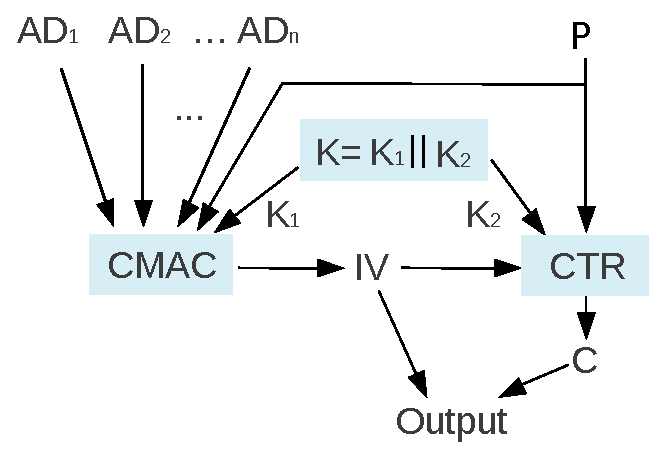
\includegraphics[scale=0.7]{./images/SIV_Encryption}
\caption{Workflow of the SIV encryption.}\label{SIVEN}
\end{figure}
The associated data is shown as $AD_1$ through $AD_n$, IV is the
synthetic IV, the ciphertext is C \cite{SIV}. The S2V process consists
the doubling and xoring operations on the output of CMAC. CTR is a
counter mode of AES.

\subsubsection*{Generic Part}
\begin{lstlisting}{}
  generic
    with package BC is new Crypto.Symmetric.Blockcipher(<>);
    with package N is new Crypto.Types.Nonces(BC.Block);
    with function "xor" (Left, Right : in BC.Block)
    										return BC.Block is <>;
    with function To_Block_Type (B : Bytes) return BC.Block;
    with function To_Bytes (B : BC.Block) return Bytes;
    with function Shift_Left (Value: BC.Block; Amount: Natural)
    										return BC.Block;
    with function "+" (Left: BC.Block; Right : in Byte)
    										return BC.Block is <>;
\end{lstlisting}

\subsubsection*{Types}
\begin{lstlisting}{}
 type AEAD_SIV is new AE.AE_Scheme and AEAD.AEAD_Scheme with private;
\end{lstlisting}

\subsubsection*{Procedures}
\begin{lstlisting}{}
  procedure Init_Enc(This   : out    AEAD_SIV;
                     Key1   : in     Key_Type;
                     Key2   : in     Key_Type);
  procedure Init_Dec(This   : out    AEAD_SIV;
                     Key1   : in     Key_Type;
                     Key2   : in     Key_Type);
  overriding
  procedure Encrypt(This             : in out AEAD_SIV;
                    Read_Plaintext   : in     Callback_Reader;
                    Write_Ciphertext : in     Callback_Writer);
  overriding
  procedure Encrypt(This             : in out AEAD_SIV;
                    Read_Header      : in     Callback_Reader;
                    Read_Plaintext   : in     Callback_Reader;
                    Write_Ciphertext : in     Callback_Writer);
  overriding
  function Decrypt_And_Verify(This      : in out AEAD_SIV;
                 Read_Ciphertext        : in Callback_Reader;
                 Read_Ciphertext_Again  : in Callback_Reader := null;
                 Write_Plaintext        : in Callback_Writer)
                     							return Boolean;
  overriding
  function Decrypt_And_Verify(This      : in out AEAD_SIV;
                 Read_Header            : in Callback_Reader;
                 Read_Ciphertext        : in Callback_Reader;
                 Read_Ciphertext_Again  : in Callback_Reader := null;
                 Write_Plaintext        : in Callback_Writer)
                               				return Boolean;
\end{lstlisting}
In preparation the key is set into two subkeys, which work in S2V and
CTR processes respectively. IV is used in CTR and also makes up the
final output as $IV||C$.

\subsubsection*{Example}
\begin{lstlisting}{}
  --Before calling the main program,
  --the interface functions should be implemented.
  procedure Example_SIV(T:in out Test_Cases.Test_Case'Class) is
    use AUnit.Assertions;
  begin
    SIV.Init_Enc(This => SIV_Type, Key1 => K1, Key2 => K2);
    SIV.Encrypt(This => SIV_Type, Read_Header => RH,
                Read_Plaintext => RP, Write_Ciphertext => WC);
    Put_Line("Ciphertext:");
    for I in 1..Natural(C_Vector.Length) loop
      Put(C_Vector.Element(I));
    end loop;
    C_Vector2 := C_Vector;
    Header_Index := 0;
    SIV.Init_Dec(This => SIV_Type, Key1 => K1, Key2 => K2);
    Verification_Bool := SIV.Decrypt_And_Verify
                      (This => SIV_Type, Read_Header => RH,
                       Read_Ciphertext => RC,
                       Read_Ciphertext_Again => RCA,
                       Write_Plaintext => WP);
    Put_Line(Verification_Bool'Img);
    if Verification_Bool then
      Put_Line("Plaintext:");
      for I in 1..Natural(Plain_Array.Length) loop
         Put(Plain_Array.Element(I));
      end loop;
    end if;
  end Example_SIV;
\end{lstlisting}

\chapter{Acl.Crypto.Asymmetric}

\subsubsection{Beschreibung}
Dies ist das Wurzelpaket f�r die asymmetrische Kryptographie.\\

\subsubsection{Funktion}
Dieses Paket erm�glicht dem symmetrischen Teil den direkten Zugriff auf 
Crypto.Types, welches grundlegende Typen und deren Basisfunktionen zur 
Verf�gung stellt. Des weiteren  erm�glicht diese Paket  dem asymmetrischen Teil
den Zugriff auf Crypto.Types.Big\_Numbers.

\section{Exceptions}
\begin{lstlisting}{}
  Invalid_Private_Key_Error : exception;
  Invalid_Public_Key_Error  : exception;
  Plaintext_Too_Long_Error  : exception;
  Decrypt_Error             : exception;
\end{lstlisting}

\chapter{Acl.Crypto.Asymmetric.RSA}

Bei diesem generischen Paket handelt es sich um eine RSA 
(Rivest Shamir Adelman) Implementierung. Klartextbl�cke (Plaintext) bzw.
Chiffretextbl�cke (Ciphertext) k�nnen mit Hilfe von RSAES-OAEP \cite{rsa}
ver- bzw. entschl�sselt werden. RSAES-PKCS1-v1\_5 wurde nicht implementiert, da
im PKCS \#1 v2.1 (Public-Key Cryptography Standards) empfohlen wird f�r
neue Anwendungen RSAES-OEAP zu verwenden.\\

\subsubsection{OEAP-Details}
\begin{itemize}
\item Diese Implementation verwendet SHA1 innerhalb der MGF1\\
  (Mask Generation Function 1)
\item Diese Implementation unterst�zt nicht das optionale Label L, d.h. L ist
  immer ein leerer String
\end{itemize}


\section{Generischer Teil}
\begin{lstlisting}{}
generic
  Size : Positive;
\end{lstlisting}\ \\
\textbf{Vorbedingung:}\\
Size $\ge$512\\ \ \\
\textbf{Exception:}\\
Size $<$ 512  : Constraint\_Size\_Error;\\

%%%%%%%%%%%%%%%%%%%%%%%%%%%%%%%%%%%%%%%%%%%%%%%%%%%%%%%%%%%%%%%%%%%%%%%%%%%
%%%%%%%%%%%%%%%%%%%%%%%%%%%%%%%%%%%%%%%%%%%%%%%%%%%%%%%%%%%%%%%%%%%%%%%%%%%

\section{API}
\subsection{Typen}
\begin{lstlisting}{}
 subtype RSA_Number is Bytes(0..Size/8-1);
 type Public_Key_RSA  is private;
 type Private_Key_RSA is private;
\end{lstlisting}
Bei RSA\_Number handeltes sich um ein Byte-Array das als Zahl interpretiert
wird. Das erste Element des Arrays (First) enstpricht dabei dem 
dem h�chstwertigsten Byte und das letzte Element des Arrays (Last)
dem niederwertigsten Byte dieser Zahl.\\ \ \\

%%%%%%%%%%%%%%%%%%%%%%%%%%%%%%%%%%%%%%%%%%%%%%%%%%%%%%%%%%%%%%%%%%%%%%%%%%%
%%%%%%%%%%%%%%%%%%%%%%%%%%%%%%%%%%%%%%%%%%%%%%%%%%%%%%%%%%%%%%%%%%%%%%%%%%%

\subsection{Prozeduren und Funktionen}\ 

\begin{tabular}{p{\textwidth}}
\begin{lstlisting}{}
  procedure Gen_Key(Public_Key    : out Public_Key_RSA;
                      Private_Key : out Private_Key_RSA);
\end{lstlisting}\\
Dies Prozedure erzeugt ein Schl�sselpaar, das aus einem  �ffentlichen 
\textit{Public\_Key} und einem privaten Schl�ssel \textit{Private\_Key}
besteht.\\ \ \\
\hline
\end{tabular}

%%%%%%%%%%%%%%%%%%%%%%%%%%%%%%%%%%%%%%%%%%%%%%%%%%%%%%%%%%%%%%%%%%%%%%%%%%%


\begin{tabular}{p{\textwidth}}\label{rsavkp}
\begin{lstlisting}{}
 function Verify_Key_Pair(Private_Key  : Private_Key_RSA;
                           Public_Key  : Public_Key_RSA) return Boolean;
\end{lstlisting}\\
Diese Funkton gibt ``True'' zur�ck, wenn der privaten \textit{Private\_Key}
und der �ffentliche Schl�ssel \textit{Public\_Key} zusammengeh�ren, d.h. ein 
Paar bilden, ansonsten gibt sie ``False'' zur�ck. \\ \ \\
\textbf{Exception:}\\
\begin{tabular}{l @{\ :\ } l}
  Public\_Key  wurde nicht initalisiert & Invalid\_Public\_Key\_RSA\\
  Private\_Key wurde nicht initalisiert & Invalid\_Private\_Key\_RSA\\
\end{tabular}\\ \ \\
\hline
\end{tabular}

%%%%%%%%%%%%%%%%%%%%%%%%%%%%%%%%%%%%%%%%%%%%%%%%%%%%%%%%%%%%%%%%%%%%%%%%%%%

\begin{tabular}{p{\textwidth}}
\begin{lstlisting}{}
 function OAEP_Encrypt(Public_Key : in  Public_Key_RSA;
                         Plaintext  : in  Bytes) return RSA_Number;
\end{lstlisting}
Diese Funktion verschl�sselt einen Klartext(-block) (\textit{Plaintext})
mit dem OEAP-Verfahren \cite{rsa} und gibt den Chiffretext zur�ck.\\ \ \\
\textbf{Vorbedingung:}\\
\textit{Plaintext'Length} $\le Size - 336 (= 2 \cdot 160 + 2\cdot 8)$\\
\textit{Public\_Key} is ein zul�ssiger Schl�ssel.\\ \ \\
\textbf{Exceptions:}\\
\begin{tabular}{l@{\ : \ }l}
  Plaintext'Length $>$ Size - 336 & Plaintext\_Too\_Long\_Error\\ 
  Public\_Key wurde nicht initalisiert & Invalid\_Public\_Key\_Error\\
  Unzul�ssiger Public\_Key & Invalid\_Public\_Key\_Error\\
\end{tabular}\ \\ \ \\
\hline
\end{tabular}

%%%%%%%%%%%%%%%%%%%%%%%%%%%%%%%%%%%%%%%%%%%%%%%%%%%%%%%%%%%%%%%%%%%%%%%%%%%

\begin{tabular}{p{\textwidth}}
\begin{lstlisting}{}
function OAEP_Decrypt(Private_Key : in  Private_Key_RSA;
                         Ciphertext  : in  RSA_Number) return Bytes;
\end{lstlisting}
Diese Funktion entschl�sselt einen Chiffretext(-block)  (\textit{Ciphertext}),
mit Hilfe eines privaten Schl�ssels (\textit{Private\_Key}). 
Der entschl�sselte Text entspricht nur dem ``orginal'' Klartext,
wenn der dabei benutze �ffentliche Schl�ssel und 
\textit{Private\_Key} ein Schl�sselpaar bilden (\ref{rsavkp}).\\
\ \\
\textbf{Vorbedingungen:}
\begin{itemize}
\item \textit{Private\_Key} ist ein zul�ssiger Schl�ssel.
\item \textit{Ciphertext} wurde mit dem RSAES-OEAP-Verfahren verschl�sselt.
\item Der �ffenltiche Schl�ssel mit dem \textit{Ciphertext} 
  verschl�sselt wurde und \textit{Private\_Key} bilden ein Schl�sselpaar.
\end{itemize}\ \\
\textbf{Exception:}\\ 
Verletzung einer Vorbedingung : Decrypt\_Error\\ \ \\
\hline
\end{tabular}

%%%%%%%%%%%%%%%%%%%%%%%%%%%%%%%%%%%%%%%%%%%%%%%%%%%%%%%%%%%%%%%%%%%%%%%%%%%

\begin{tabular}{p{\textwidth}}
\begin{lstlisting}{}
 procedure Get_Public_Key(Public_Key : in Public_Key_RSA;
                            N : out RSA_Number;
                            E : out RSA_Number);
\end{lstlisting}
Diese Prozedur zerlegt einen �ffentlichen Schl�ssel \textit{Public\_Key} 
in folgende Komponenten:
\begin{itemize}
\item Einen Size-Bit-RSA-Modulus N. (N = PQ \quad P,Q Prime)
\item Einen �ffentlichen RSA-Exponenten E.
\end{itemize}\ \\
Mit Hilfe dieser Werte l�sst sich der �ffentliche Schl�ssel zu einem sp�teren 
Zeitpunkt wieder rekonstruieren.\\ \ \\
\hline
\end{tabular}

%%%%%%%%%%%%%%%%%%%%%%%%%%%%%%%%%%%%%%%%%%%%%%%%%%%%%%%%%%%%%%%%%%%%%%%%%%%

\begin{tabular}{p{\textwidth}}
\begin{lstlisting}{}
  procedure Get_Private_Key(Private_Key : in Private_Key_RSA;
                             N   : out RSA_Number;
                             D   : out RSA_Number;
                             Phi : out RSA_Number);
\end{lstlisting}
Diese Prozedur zerlegt einen privaten Schl�ssel \textit{Private\_Key} 
in folgende Komponenten:
\begin{itemize}
\item Einen Size-Bit-RSA-Modulus N. (N = PQ \quad P,Q Prim)
\item Einen privaten RSA-Exponenten D.
\item Phi = (P-1)(Q-1). 
\end{itemize}\ \\
Mit Hilfe dieser Werte l�sst sich der private Schl�ssel zu einem sp�teren 
Zeitpunkt wieder rekonstruieren.\\ \ \\
\hline
\end{tabular}

%%%%%%%%%%%%%%%%%%%%%%%%%%%%%%%%%%%%%%%%%%%%%%%%%%%%%%%%%%%%%%%%%%%%%%%%%%%

\begin{tabular}{p{\textwidth}}
  \begin{lstlisting}{}
 procedure Set_Public_Key(N : in RSA_Number;
                            E : in RSA_Number;
                            Public_Key : out Public_Key_RSA);
  \end{lstlisting}
Mit Hilfe dieser Prozedur ist es m�glich einen �ffentlichen Schl�ssel 
\textit{Public\_Key} zu (re-)konstruieren. Man ben�tigt dazu folgende 
Werte:
\begin{itemize}
\item Einen Size-Bit-RSA-Modulus \textit{N}.
\item Einen �ffentlichen RSA-Exponenten \textit{E}.
\end{itemize}\ \\
\textbf{Exception:}\\
N oder E unzul�ssig  : Invalid\_Public\_Key\_Error.\\ \ \\
\hline
\end{tabular}


%%%%%%%%%%%%%%%%%%%%%%%%%%%%%%%%%%%%%%%%%%%%%%%%%%%%%%%%%%%%%%%%%%%%%%%%%%%

\begin{tabular}{p{\textwidth}}
  \begin{lstlisting}{}
 procedure Set_Private_Key(N   : in RSA_Number;
                             D   : in RSA_Number;
                             Phi : in RSA_Number;
                             Private_Key : out Private_Key_RSA);

  \end{lstlisting}
  Mit Hilfe dieser Prozedur ist es m�glich einen privaten Schl�ssel 
  \textit{Private\_Key} zu (re-)konstruieren. Man ben�tigt dazu folgende 
  Werte:
\begin{itemize}
\item Einen Size-Bit-RSA-Modulus \textit{N}. (\textit{N} = PQ \quad P,Q Prim)
\item Einen privaten RSA-Exponenten \textit{D}.
\item Phi = (P-1)(Q-1). 
\end{itemize}\ \\
\textbf{Exception:}\\
N, D oder S unzul�ssig : Invalid\_Public\_Key\_Error.\\ \ \\
\end{tabular}


%%%%%%%%%%%%%%%%%%%%%%%%%%%%%%%%%%%%%%%%%%%%%%%%%%%%%%%%%%%%%%%%%%%%%%%%%%%

\subsection{Low-Level-API}
Diese API sollten sie nur verwenden, wenn Sie wissen was Sie tun.
Bei einem naiven Einsatz k�nnen kritische Sicherheitsprobleme auftreten, da
identische Klartexte zu identischen Chiffretexten verschl�sselt werden.

\begin{tabular}{p{\textwidth}}
  \begin{lstlisting}{}
  procedure Encrypt(Public_Key : in  Public_Key_RSA;
                     Plaintext  : in  RSA_Number;
                     Ciphertext : out RSA_Number);
  \end{lstlisting}
  Diese Prozedur verschl�sselt einen Klartext  (\textit{Plaintext}) mit
  Hilfe eines �ffentlichen Schl�ssels (\textit{Public\_Key}) zu einem
  Chiffretext (\textit{Ciphertext}). Sie verwendet dabei das ``naive'' 
  RSA-Verfahren ($c = p^d \pmod{n}$). \\ \ \\
  \hline
\end{tabular}

%%%%%%%%%%%%%%%%%%%%%%%%%%%%%%%%%%%%%%%%%%%%%%%%%%%%%%%%%%%%%%%%%%%%%%%%%%%

\begin{tabular}{p{\textwidth}}
  \begin{lstlisting}{}
  procedure Decrypt(Private_Key : in  Private_Key_RSA;
                      Ciphertext  : in  RSA_Number;
                      Plaintext   : out RSA_Number);
  \end{lstlisting}
  Diese Prozedur entschl�sselt einen Chiffretext  (\textit{Ciphertext}) mit
  Hilfe eines privaten Schl�ssels (\textit{Private\_Key}) zu einem
  Klartext  (\textit{Plaintext}). Sie verwendet dabei das ``naive'' 
  RSA-Verfahren ($p = c^e \pmod{n}$). \\ \ \\
\end{tabular}\ \\

\subsection{Anwendungsbeispiel}
\begin{lstlisting}{}
with Crypto.Types;
with Crypto.Asymmetric.RSA;
with Ada.Text_IO;

procedure Example_RSA is
   package RSA is new Crypto.Asymmetric.RSA(512);
   use Crypto.Types;
   use Ada.Text_IO;
   use RSA;

   Message : Bytes := To_Bytes("All your base...");
   Public_Key  : Public_Key_RSA;
   Private_Key : Private_Key_RSA;

begin
   --Generierung des Schluesselpaares
   Gen_Key(Public_Key, Private_Key);

   declare
      --Verschluesselung
      Ciphertext : RSA_Number := OAEP_Encrypt(Public_Key, Message);

      -- Entschluesselung
      Plaintext : Bytes := OAEP_Decrypt(Private_Key, Ciphertext);

   begin
      -- Ausgabe des Chiffretextes
      Put(To_String(Ciphertext)); New_Line;

      -- Ausgabe des entschluesselten Chiffretextes
      Put(To_String(Plaintext));
   end;
end Example_RSA;
\end{lstlisting}


\chapter{Acl.Crypto.Asymmetric.DSA}

Bei diesem generischen Paket handelt es sich um eine Implementierung des
DSA-Signaturalgorithmus. Der DSA-Algorithmus ist Teil des digitalen Signatur
Standards (DSS) \cite{dss} der von der NSA entworfen und 1994 vom NIST 
verabschiedet wurde. Die Bezeichner wurden aus dem DSS �bernommen.\\
Mit Hilfe von DSA sind Sie  in der Lage digitale Unterschriften zu 
erstellen und deren Authentizit�t zu verifizieren. 
Um eine Nachricht digital zu unterschreiben (signieren) ben�tigt Sie einen 
�ffentlichen und einen privaten Schl�ssel.
Den privaten Schl�ssel ben�tigt Sie f�r den Signierungsprozess und den 
�ffentlichen Schl�ssel f�r den Verifikationsprozess. Bei diesen Prozessen
wird nicht die Nachricht selbst sondern deren SHA-1 Hash-Wert 
\ref{sha1} unterschrieben. Jemand der den privaten Schl�ssel nicht kennt, ist 
nicht in der Lage eine g�ltige (verifizierbare) Signatur zu erstellen.
Aber jeder der den �ffentlichen Schl�ssel kennt, kann sich von der Korrektheit
einer Signatur �berzeugen indem er sie dem Verifizierungsprozess unterwirft.


\section{Generischer Teil}
\begin{lstlisting}{}
generic
  Size : Positive;
\end{lstlisting}\ \\
\textbf{Exception}
$Size \not= 512+i64 \quad (i \in \{0, \ldots , 8\})$ : Constraint\_Error;\\

\section{API}
\subsection{Typen}
\begin{lstlisting}{}
 subtype DSA_Number is Bytes(0..Size/8-1);
 type Public_Key_DSA  is private;
 type Private_Key_DSA is private;
 type Signature_DSA   is private;
\end{lstlisting}
Bei DSA\_Number handeltes sich um ein Byte-Array das als Zahl interpretiert
wird. Das erste Element des Arrays (First) enstpricht dabei dem 
dem h�chstwertigsten Byte und das letzte Element des Arrays (Last)
dem niederwertigsten Byte dieser Zahl.\\ \ \\

\subsection{Prozeduren und Funktionen}
\begin{tabular}{p{\textwidth}}
\begin{lstlisting}{}
procedure Gen_Key(Public_Key  : out Public_Key_DSA;
                     Private_Key : out Private_Key_DSA);
\end{lstlisting}\\
Diese Prozedur erzeugt ein Schl�sselpaar, das aus einem �ffentlichen 
\textit{Public\_Key} und einem privaten Schl�ssel \textit{Private\_Key}
besteht.\\ \ \\
\hline
\end{tabular}


%%%%%%%%%%%%%%%%%%%%%%%%%%%%%%%%%%%%%%%%%%%%%%%%%%%%%%%%%%%%%%%%%%%%%%%%%%%


\begin{tabular}{p{\textwidth}}
\begin{lstlisting}{}
procedure Sign(Private_Key   : in  Private_Key_DSA;
                 SHA1_Hash   : in  W_Block160;
                 Signature   : out Signature_DSA);
\end{lstlisting}\\
Diese Prozedur signiert den SHA-1 Hashwert (\textit{SHA1\_Hash}) einer
Nachricht mit einem privaten Schl�ssel (\textit{Private\_Key}).\\ \ \\
\hline
\end{tabular}

%%%%%%%%%%%%%%%%%%%%%%%%%%%%%%%%%%%%%%%%%%%%%%%%%%%%%%%%%%%%%%%%%%%%%%%%%%%

\begin{tabular}{p{\textwidth}}
\begin{lstlisting}{}
function Verify(Public_Key  : Public_Key_DSA;
                 SHA1_Hash   : W_Block160;
                 Signature   : Signature_DSA) return Boolean;
\end{lstlisting}\\
Diese Funktion gibt den Wert ``True'' zur�ck, wenn mit Hilfe des �ffentlichen
Schl�ssels \textit{Public\_Key} verifiziert werden kann,
ob es sich bei \textit{Signature} um eine g�ltige Unterschrift des SHA-1
Hashwertes \textit{SHA1\_Hash} handelt.
Ist dies nicht der Fall gibt sie ``False'' zur�ck.\\
Mit einem �ffentlichen Schl�ssel, k�nnen nur Signaturen des zugeh�rigen
privaten Schl�ssels verifiziert werden. Passen die beiden Schl�ssel nicht 
zusammen, gibt diese Funktion ``False'' zur�ck.\\
Wenn Bob anstatt seines den Ausweis den von Alice mit sich f�hrt, dann kann 
man anhand dieses Ausweises auch nicht die Identit�t von  Bob �berpr�fen, 
obwohl Alice Ausweis g�ltig ist. \\ \ \\
\hline
\end{tabular}

%%%%%%%%%%%%%%%%%%%%%%%%%%%%%%%%%%%%%%%%%%%%%%%%%%%%%%%%%%%%%%%%%%%%%%%%%%%

\begin{tabular}{p{\textwidth}}
\begin{lstlisting}{}
procedure Sign_File(Filename      : in  String;
                      Private_Key : in  Private_Key_DSA;
                      Signature   : out Signature_DSA);
\end{lstlisting}\\
Mit dieser Prozedur kann man mit Hilfe eines privaten Schl�ssels 
\textit{Private\_Key} eine Datei (\textit{Filename}) signieren.\\ \ \\
\textbf{Exception:}\\
\begin{tabular}{l @{\ :\ } l}
  Die Datei \textit{Filename} ist gr��er als $2^{26}$ TB & 
  SHA1\_Constraint\_Error\\
  Private\_Key wurde nicht initialisiert & Invalid\_Private\_Key\\
  Lesefehler & File\_Open\_Error\\
\end{tabular}\ \\ \ \\
\hline
\end{tabular}

%%%%%%%%%%%%%%%%%%%%%%%%%%%%%%%%%%%%%%%%%%%%%%%%%%%%%%%%%%%%%%%%%%%%%%%%%%%

\begin{tabular}{p{\textwidth}}
\begin{lstlisting}{}
function Verify_File(Filename    : String;
                      Public_Key : Public_Key_DSA;
                      Signature  : Signature_DSA) return Boolean;
\end{lstlisting}\\
Diese Funktion gibt den Wert ``True'' zur�ck, wenn mit Hilfe des �ffentlichen
Schl�ssels \textit{Public\_Key} verifiziert werden kann, ob es sich bei
\textit{Signature} um eine g�ltige Unterschrift der Datei (\textit{Filename})
handelt. Ist dies nicht der Fall gibt sie ``False'' zur�ck.\\
Mit einem �ffentlichen Schl�ssel, k�nnen nur Signaturen des dazugeh�rigen
privaten Schl�ssels verifiziert werden. Passen die beiden Schl�ssel nicht 
zusammen, gibt diese Funktion ``False'' zur�ck.\\ \ \\
\textbf{Exception:}\\
\begin{tabular}{l @{\ :\ }l}
Die Datei \textit{Filename} ist gr��er als $2^{26}$ TB & 
SHA1\_Constraint\_Error\\
Public\_Key  wurde nicht initialisiert  & Invalid\_Public\_Key\\
Lesefehler & File\_Open\_Error\\
\end{tabular}\ \\ \ \\
\hline
\end{tabular}

%%%%%%%%%%%%%%%%%%%%%%%%%%%%%%%%%%%%%%%%%%%%%%%%%%%%%%%%%%%%%%%%%%%%%%%%%%%

\begin{tabular}{p{\textwidth}}
\begin{lstlisting}{}
  function Verify_Key_Pair(Private_Key : Private_Key_DSA;
                            Public_Key  : Public_Key_DSA) return Boolean;
\end{lstlisting}\\
Diese Funktion gibt ``True'' zur�ck, wenn der privaten \textit{Private\_Key}
und der �ffentliche Schl�ssel \textit{Public\_Key} zusammengeh�ren, d.h. ein 
Paar bilden, ansonsten gibt sie ``False'' zur�ck. \\ \ \\
\textbf{Exception:}\\
\begin{tabular}{l @{\ :\ } l}
  Public\_Key  wurde nicht initialisiert & Invalid\_Public\_Key\_Error\\
  Private\_Key wurde nicht initialisiert & Invalid\_Private\_Key\_Error\\
\end{tabular}\\ \ \\
\hline
\end{tabular}


%%%%%%%%%%%%%%%%%%%%%%%%%%%%%%%%%%%%%%%%%%%%%%%%%%%%%%%%%%%%%%%%%%%%%%%%%%%

\begin{tabular}{p{\textwidth}}
\begin{lstlisting}{}
   procedure Get_Public_Key(Public_Key : in Public_Key_DSA;
                            P : out DSA_Number;
                            Q : out DSA_Number;
                            G : out DSA_Number;
                            Y : out DSA_Number);
\end{lstlisting}\\
Diese Prozedur zerlegt einen �ffentlichen Schl�ssel \textit{Public\_Key} 
in folgende Komponenten:
\begin{itemize}
\item Eine Size-Bit-Primzahl P.
\item Eine 160-Bit-Primzahl Q.
\item Einen Generator G der eine Untergruppe von P mit der Ordnung Q erzeugt.
\item Der eigentliche �ffentliche Schl�ssel Y. 
\end{itemize}\ \\
Mit Hilfe dieser Werte l�sst sich der �ffentliche Schl�ssel zu einem sp�teren 
Zeitpunkt wieder rekonstruieren.\\ \ \\
\hline
\end{tabular}

%%%%%%%%%%%%%%%%%%%%%%%%%%%%%%%%%%%%%%%%%%%%%%%%%%%%%%%%%%%%%%%%%%%%%%%%%%%

\begin{tabular}{p{\textwidth}}
\begin{lstlisting}{}
 procedure Get_Private_Key(Private_Key : in Private_Key_DSA;
                             P : out DSA_Number;
                             Q : out DSA_Number;
                             G : out DSA_Number;
                             X : out DSA_Number);
\end{lstlisting}\\
Diese Prozedur zerlegt einen privaten Schl�ssel \textit{Private\_Key} 
in folgende Komponenten:
\begin{itemize}
\item Eine Size-Bit-Primzahl P.
\item Eine 160-Bit-Primzahl Q.
\item Einen Generator G der eine Untergruppe von P mit der Ordnung Q erzeugt.
\item Der eigentliche geheime Schl�ssel X. 
\end{itemize}\ \\
Mit Hilfe dieser Werte l�sst sich der private Schl�ssel zu einem sp�teren 
Zeitpunkt wieder rekonstruieren.\\ \ \\
\hline
\end{tabular}

%%%%%%%%%%%%%%%%%%%%%%%%%%%%%%%%%%%%%%%%%%%%%%%%%%%%%%%%%%%%%%%%%%%%%%%%%%%

\begin{tabular}{p{\textwidth}}
\begin{lstlisting}{}
  procedure Set_Public_Key(P : in DSA_Number;
                            Q : in DSA_Number;
                            G : in DSA_Number;
                            Y : in DSA_Number;
                            Public_Key : out Public_Key_DSA);
\end{lstlisting}\\
Mit Hilfe dieser Prozedur ist es m�glich einen �ffentlichen Schl�ssel 
\textit{Public\_Key} zu (re-)konstruieren. Man ben�tigt dazu folgende 
Werte:
\begin{itemize}
\item Eine Size-Bit-Primzahl \textit{P}.
\item Eine 160-Bit-Primzahl \textit{Q}.
\item Einen Generator \textit{G} der eine Untergruppe von $ Z_P^*$  mit der
  Ordnung \textit{Q} erzeugt.
\item Den eigentliche �ffentlichen Schl�ssel \textit{Y}.
\end{itemize}\ \\
\textbf{Exception:}\\
P, Q, G oder Y unzul�ssig : Invalid\_Public\_Key\_Error.\\ \ \\
\hline
\end{tabular}

%%%%%%%%%%%%%%%%%%%%%%%%%%%%%%%%%%%%%%%%%%%%%%%%%%%%%%%%%%%%%%%%%%%%%%%%%%%

\begin{tabular}{p{\textwidth}}
\begin{lstlisting}{}
 procedure Set_Private_Key(P : in DSA_Number;
                             Q : in DSA_Number;
                             G : in DSA_Number;
                             X : in DSA_Number;
                             Private_Key : out Private_Key_DSA);
\end{lstlisting}\\
Mit Hilfe dieser Prozedur ist es m�glich einen privaten Schl�ssel 
(\textit{Private\_key}) zu (re-)konstruieren. Man ben�tigt dazu folgende 
Werte:
\begin{itemize}
\item Eine Size-Bit-Primzahl \textit{P}.
\item Eine 160-Bit-Primzahl \textit{Q}.
\item Einen Generator \textit{G} der eine Untergruppe von $ Z_P^*$  mit der
  Ordnung \textit{Q} erzeugt.
\item Den eigentliche geheime Schl�ssel \textit{X}.
\end{itemize}\ \\
\textbf{Exception:}\\
P, Q, G oder Y unzul�ssig : Invalid\_Private\_Key\_Error.\\ \ \\
\end{tabular}


%%%%%%%%%%%%%%%%%%%%%%%%%%%%%%%%%%%%%%%%%%%%%%%%%%%%%%%%%%%%%%%%%%%%%%%%%%%

\section{Anwendungsbeispiel}
\begin{lstlisting}{}
with Crypto.Types.Big_Numbers;
with Crypto.Asymmetric.Dsa;
with Ada.Text_IO; use Ada.Text_IO;

procedure Example_DSA is
   package DSA is new Crypto.Asymmetric.DSA(512);
   use DSA;

   Public_Key  : Public_Key_DSA;
   Private_Key : Private_Key_DSA;
   Signature   : Signature_DSA;

begin
   --Schluesselgenerierung
   Gen_Key(Public_Key, Private_Key);

   --Signierung
   Sign_File("example_dsa.adb", Private_Key, Signature);

   --Verifikation
   if Verify_File("example_dsa.adb", Public_Key, Signature) then
        Put_Line("OK");
   else Put_Line("Implementation error.");
   end if;

end Example_DSA;
\end{lstlisting}

\chapter{Crypto.Asymmetric.ECDSA}
In this generic package the ECDSA (Elliptic Curve DSA) algorithm is implemented. It's a further extension of the DSA algorithm in the area of elliptic curve. Users can generate digital signatures and verify the authenticity of the signatures by using ECDSA. The private key is used in the signature process, while the public key is used for verification. During the signature process the SHA-1 hash value of the message (not the message) is signed. People who hasn't the private key can't generate a valid signature. However people who knows the public key can convince the signature by running the verification process.
\section{API}
\subsubsection*{Generic Part}
\begin{lstlisting}{}
  generic
    Size : Positive;
\end{lstlisting}
\subsubsection*{Types}
\begin{lstlisting}{}
  type Public_Key_ECDSA is private;
  type Private_Key_ECDSA is private;
  type Signature_ECDSA is private;
\end{lstlisting}
The type \texttt{Public\_Key\_ECDSA} has four components:
\begin{lstlisting}{}
  type ECDSA_P_KEY is record
    E : Elliptic_Curve_Zp;
    P : EC_Point; 
    n : Big_Unsigned;
    Q : EC_Point; 
  end record;
  type Public_Key_ECDSA is new ECDSA_P_KEY;
\end{lstlisting}
$E$ is an elliptic curve over $Z_P$. $P$ is a public point in the curve, and its order is known as $n$. $Q$ is the public part of the key. \\
The type \texttt{Private\_Key\_ECDSA} has the following variables:
\begin{lstlisting}{}
  type ECDSA_S_KEY is record
    Q : EC_Point; 
    d : Big_Unsigned;
  end record;
  type Private_Key_ECDSA is new ECDSA_S_KEY;
\end{lstlisting}
$Q$ is a point in the elliptic curve and also the public part of the key. $d$ is a number and the private part of the key.\\
The type \texttt{Signature\_ECDSA} contains the following variables:
\begin{lstlisting}{}
  type ECDSA_KEY is record
    R : Big_Unsigned;
    S : Big_Unsigned;
  end record;
  type Signature_ECDSA is new ECDSA_KEY;
\end{lstlisting}
The signature is made of a pair ($R,S$).\\
\subsection*{Procedures}
\begin{lstlisting}{}
  procedure Gen_Public_Key(Public_Key  : out Public_Key_ECDSA;
			               	length      : in DB.Bit_Length);
\end{lstlisting}
This procedure gets an elliptic curve from the database. The curve has at least cryptographic security in length.\\
\hline \\ \ \\
\begin{lstlisting}{}
 procedure Gen_Private_Key(Public_Key :in out Public_Key_ECDSA;
                           Private_Key:out Private_Key_ECDSA);
\end{lstlisting}
This procedure generates a private key corresponding to the previously created public key. A random number ($d$) will be produced at first as the secret part of the key. Then a point ($Q$) is calculated as common part of the two keys (it is stored in both keys) from the random number ($d$) and the public point of the public key ($P$).\\
\hline \\ \ \\
\begin{lstlisting}{}
  procedure Sign(Public_Key  : in Public_Key_ECDSA;
		 			  Private_Key : in  Private_Key_ECDSA;
                 SHA1_Hash   : in  W_Block160;
                 Signature   : out Signature_ECDSA);
\end{lstlisting}
This procedure signs the SHA-1 hash value of a message with the private key.\\
\hline \\ \ \\
\begin{lstlisting}{}
  function Verify(Public_Key  : Public_Key_ECDSA;
                  SHA1_Hash   : W_Block160;
                  Signature   : Signature_ECDSA)
                  return Boolean;
\end{lstlisting}
The function returns true if the signature can be verified with the public key to be a valid signature of the SHA-1 hash value \texttt{SHA1\_Hash}. If not, then false will be returned.\\
With the public key only the signature which related to the private key can be verified. If the two keys don't match together, then false\begin{scriptsize}
•
\end{scriptsize} will be returned.\\
But consider this situation, if Bob uses the identity card of Alice, then we can't make identification of Bob with the identity card, although the identity card of Alice is valid.\\
\hline \\ \ \\
\begin{lstlisting}{}
  procedure Sign_File(Filename    : in  String;
          		       Public_Key  : in  Public_Key_ECDSA;
					     	 Private_Key : in  Private_Key_ECDSA;
						    Signature   : out Signature_ECDSA);
\end{lstlisting}
This procedure signs data file (\texttt{Filename}) with the private key.\\
\textbf{Exception:}
If the \texttt{Private\_Key} is not initialized:\quad \texttt{Invalid\_Private\_Key\_Error}.\\
\hline \\ \ \\
\begin{lstlisting}{}
  function Verify_File(Filename   : String;
					 		  Public_Key : Public_Key_ECDSA;
                       Signature  : Signature_ECDSA) 
                       return Boolean;
\end{lstlisting}
This function returns true if the signature can be verified with the public key to be a valid signature of the file (\texttt{Filename}). If not, then false will be returned.\\
Only the signature which related to the private key and the public key can be verified. If the two keys don't match, then false will be returned.\\
\textbf{Exception:}
If the \texttt{Public\_Key} is not initialized:\quad \texttt{Invalid\_Public\_Key\_Error}.\\
\hline \\ \ \\
\begin{lstlisting}{}
  function Verify_Key_Pair(Private_Key : Private_Key_ECDSA;
                           Public_Key  : Public_Key_ECDSA) 
                           return Boolean;
\end{lstlisting}
This function returns true if the private key and the public key match, that is, they are verified to be a pair of keys. If not, false is returned.\\
\hline \\ \ \\
\begin{lstlisting}{}
  function equal_Public_Key_Curve
  					  					(Public_Key_A : Public_Key_ECDSA;
		              				 Public_Key_B : Public_Key_ECDSA) 	
								 			return Boolean;
\end{lstlisting}
This function returns true if the two public keys, \texttt{Public\_Key\_A} and \texttt{Public\_Key\_B}, are tested to be the same key, else false is returned.\\
\section{Example}
\begin{lstlisting}{}
  with Crypto.Asymmetric.ECDSA;
  with Crypto.Types.Big_Numbers;
  with Ada.Text_IO;
  use Ada.Text_IO;

  procedure Example_ECDSA is
  	package ECDSA is new Crypto.Asymmetric.ECDSA(512);
  	use ECDSA;
  	Public_Key : Public_Key_ECDSA;
  	Private_Key : Private_Key_ECDSA;
  	Signature : Signature_ECDSA;
  begin
    -- Generation
    Gen_Public_Key(Public_Key, 178);
  	 Gen_Private_Key(Public_Key, Private_Key);
  	-- Sign
  	 Sign_File("Example_DSA.adb", Public_Key, 
  	          Private_Key, Signature);
  	-- Verification
  	if Verify_File("Example_DSA.adb", Public_Key, Signature) then
       Put_Line("OK");
    else 
       Put_Line("Error");
    end if;
  end Example_ECDSA;
\end{lstlisting}

\chapter{Crypto.Asymmetric.ECDH}\label{ECDH}
In this generic package the implementation of Elliptic Curve
Diffie–Hellman (ECDH) algorithm is provided. The ECDH is an key
agreement protocol that allows two parties, each having the other
party's public key, and one's own private key, to establish a shared
secret over an insecure channel \cite{ECDH-NIST}. A brief description
of elliptic curve will be introduced here. For detailed information
you can go to \texttt{Crypto.Types.Elliptic\_Curve} (Chapter
\ref{ConceptofElliptic}).

\subsubsection*{Mathematical Background}
An elliptic curve $E$ is of the form $y^2=x^3+ax+b\mod p$. A point $P$
is in the curve $E$ and has an order $n$. A pair of keys are made of a
public point $Q$ and a secret number $d$ where $Q=d*P$. For
calculation these following parameters are required: $a,b,p,P,n$ and
also the key pair $(d,Q)$.

\subsubsection*{Key Generation}
Let Alice's key pair be ($d_A,Q_A$) and Bob's key pair be
($d_B,Q_B$). Each public part should be known to the other
party.\\ Alice compute $(x_k,y_k)=d_AQ_B$, Bob computes
$(x_k,y_k)=d_BQ_A$. The shared key is $x_k$ (the $x$ coordinate of the
point). The shared key calculated by both parties is equal,
because\\ $d_AQ_B=d_Ad_BP=d_Bd_AP=d_BQ_A$.
\section{API}
\subsubsection*{Generic Part}
\begin{lstlisting}{}
  generic
    Size : Positive;
\end{lstlisting}
\textbf{Types}
\begin{lstlisting}{}
  type Private_Key_ECDH is private;
  type Shared_Key_ECDH;
  type Public_Key_ECDH;
\end{lstlisting}
The type \texttt{Private\_Key\_ECDH} has two components:
\begin{lstlisting}{}
  type ECDH_S_KEY is record
    Q : EC_Point; 
    d : Big_Unsigned;
  end record;
  type Private_Key_ECDH is new ECDH_S_KEY;
\end{lstlisting}
$Q$ is a point in the elliptic curve and also the public part of the key. $d$ is a number and the secret part of the key.\\
The type \texttt{Shared\_Key\_ECDH} contains a point:
\begin{lstlisting}{}
  type ECDH_KEY is record
    W : EC_Point;  --(x,y) in Key Generation
  end record;
  type Shared_Key_ECDH is new ECDH_KEY;
\end{lstlisting}
The type \texttt{Public\_Key\_ECDH} is made of:
\begin{lstlisting}{}
  type ECDH_P_KEY is record
    E : Elliptic_Curve_Zp;
    P : EC_Point;
    n : Big_Unsigned;
    Q : EC_Point;
  end record;
  type Public_Key_ECDH is new ECDH_P_KEY;
\end{lstlisting}
$E$ is an elliptic curve over $Z_P$. $P$ is a public point in the
curve and is in order $n$, $Q$ is the public part of the key.

\subsubsection*{Procedures}
\begin{lstlisting}{}
  procedure Gen_Public_Key(Public_Key_A  : out Public_Key_ECDH;
			    			   	length        : in  DB.Bit_Length);
\end{lstlisting}
This procedure gets an elliptic curve from the database. The curve has
at least cryptographic security in length.\\ \hhline
\begin{lstlisting}{}
  procedure Gen_Single_Private_Key
  					 (Public_Key_A  : in out Public_Key_ECDH;
				     Private_Key_A : out    Private_Key_ECDH);
\end{lstlisting}
In this procedure, a private key \texttt{Private\_Key\_A} will be
created according to the value \texttt{Public\_Key\_A}. Additionally a
random number $d$ is generated as the secret part of
\texttt{Private\_\-Key\_A}. Then a point $Q$ is calculated as the
public part of \texttt{Private\_Key\_A} which is the product of the
random number and the public point $P$ of \texttt{Public\_Key\_A}
(that is, $Q=d*P$). Point $Q$ will be stored in both keys.\\ \hhline
\begin{lstlisting}{}
  procedure Gen_Shared_Private_Key
  					(Public_Key_B  : in Public_Key_ECDH;
				    Private_Key_A : in Private_Key_ECDH;
				    Shared_Key_A  : out Shared_Key_ECDH);
\end{lstlisting}
In this procedure a shared key \texttt{Shared\_Key\_A} is
generated. It is calculated as the product of the public part of
\texttt{Public\_Key\_B} and the secret part of
\texttt{Private\_Key\_A}, ($Q_B*d_A$).\\

\textbf{Exception:}\\
If the shared key is equal infinity:\quad \texttt{EC\_IFINITY\_EX}.\\
\hhline

\begin{lstlisting}{}
  function Verify(Public_Key_A  : Public_Key_ECDH;
		   			Public_Key_B  : Public_Key_ECDH;
		   			Private_Key_A : Private_Key_ECDH;
		   			Private_Key_B : Private_Key_ECDH;
		   			Shared_Key_A  : Shared_Key_ECDH;
		   			Shared_Key_B  : Shared_Key_ECDH) 
		   			                return Boolean;
\end{lstlisting}
This function returns true if the same private keys and shared keys
can be calculated from the delivered informations.

\section{Example}
\begin{lstlisting}{}
  with Crypto.Types.Big_Numbers;
  with Ada.Text_IO;
  with Crypto.Symmetric.Algorithm.ECDH;
  use Ada.Text_IO;
  procedure Example_ECDH is
    package ECDH is new Crypto.Symmetric.Algorithm.ECDH(512);
    use ECDH;
    Public_Key_A, Public_Key_B : Public_Key_ECDH;
    Private_Key_A, Private_Key_B : Private_Key_ECDH;
    Shared_Key_A, Shared_Key_B : Shared_Key_ECDH;
  begin
     -- Key Generation
    Gen_Public_Key(Public_Key_A, 178);
    Gen_Single_Private_Key(Public_Key_A, Private_Key_A);
    Gen_Public_Key(Public_Key_B, 178);
    Gen_Single_Private_Key(Public_Key_B, Private_Key_B);

    Gen_Shared_Private_Key(Public_Key_B,Private_Key_A,Shared_Key_A);
    Gen_Shared_Private_Key(Public_Key_A,Private_Key_B,Shared_Key_B);
    
    if Verify(Public_Key_A, Public_Key_B, Private_Key_A, 
              Private_Key_B, Shared_Key_A, Shared_Key_B) then
       Put_Line("OK");
    else 
       Put_Line("Error");
    end if;
  end Example_ECDH;
\end{lstlisting}
%%%%%%%%%%%%%%%%%%%%%%%%%%%%%%%%%%%%%%%%%%%%%%%%%%%%%%%%%%%%%%%%%%%%%%%
%%%%%%%%%%%%%%%%%%%%%%%%%%%%%%%%%%%%%%%%%%%%%%%%%%%%%%%%%%%%%%%%%%%%%%%

\chapter{Crypto.Asymmetric.ECIES}
Elliptic Curve Integrated Encryption Scheme (ECIES) is proposed by
Abdalla, Bellare and Rogaway in \cite{DBLP:conf/ctrsa/AbdallaBR01},
and is one of the two standardized IES which based on elliptic
curves. Using ECIES algorithm two parties can do encryption and
decryption with a shared private key. Usually ECDH (Chapter
\ref{ECDH}) algorithm will be used to generate the shared key.

\subsubsection*{Precondition:}
The following algorithms will be used to calculate a shared key:
\begin{itemize}
\item Hash algorithm\quad\quad : SHA-256
\item Encryption algorithm : AES-256
\item MAC algorithm\quad\quad : HMAC-SHA-256
\end{itemize}
\subsubsection*{Encryption}
\begin{enumerate}
\item Two keys are generated from the shared ECDH key, one ($k_E$) for
  encryption and the other one ($k_M$) for MAC algorithm.
\item The message $M$ is encrypted: $C=E({k_E},M)$.
\item Tag of the ciphertext is calculated: $T=MAC({k_M},C)$.
\item Output: $C||T$.
\end{enumerate}
\subsubsection*{Decryption}
\begin{enumerate}
\item Two keys ($k_E$ and $k_M$) will be generated again.
\item Use MAC to check the tag if $T'=MAC({k_M},C)$.
\item Decrypt the message: $M=D({k_E},C)$.
\end{enumerate}

\section{API}
\subsubsection*{Generic Part}
\begin{lstlisting}{}
  generic
    Size : Positive;
\end{lstlisting}
\textbf{Exception}: $Size\neq 512+64*I$ $(I\in \{0,\cdots,8\})$:
\texttt{Constraint\_Error}.
\subsubsection*{Types}
\begin{lstlisting}{}
  type Cipher_ECIES is private;
  type Plain_ECIES is private;
\end{lstlisting}
The type \texttt{Cipher\_ECIES} has five components:
\begin{lstlisting}{}
  type ECIES_C_KEY is record
    Public_Point        : EC_Point;
    Message_Block_Count : natural := 0;
    Mac                 : W_Block256;
    Cipher              : Unbounded_String;
    Cipher_Map          : Container_Cipher_Map.Map;
  end record;
  type Cipher_ECIES is new ECIES_C_KEY;
\end{lstlisting}
The term \texttt{Public\_Point} is the public
key. \texttt{Message\_Block\_Count} is used to count the ciphertext
blocks. \texttt{Mac} is the MAC tag of the ciphertext
block. \texttt{Cipher} is the ciphertext. The ciphertext is divided
into blocks, the blocks are indexed in
\texttt{Cipher\_Map}.\\ \ \\ The type \texttt{Plain\_ECIES} is made
of:
\begin{lstlisting}{}
  type ECIES_P_KEY is record
    Message_Block_Count : natural := 1;
    AES_Key             : B_Block256;
    Mac_Key             : W_Block512;
    Message             : Unbounded_String;
    Message_Map         : Container_Message_Map.Map;
  end record;
  type Plain_ECIES is new ECIES_P_KEY;
\end{lstlisting}
\texttt{Message\_Block\_Count} is the count of the message
blocks. \texttt{AES\_Key} is the key for AES-256 algorithm, and
\texttt{Mac\_Key} is the key for HMAC-SHA-256
algorithm. \texttt{Message} is the plaintext. The plaintext is divided
into blocks, and they are indexed in \texttt{Message\_Map}.\\
\subsubsection*{Procedures}
\begin{lstlisting}{}
   --internal purpose
  procedure Message_Prepare(Plain   : out Plain_ECIES;
                            Message : in  String);
\end{lstlisting}
This procedure converts a string to the type
\texttt{Plain\_ECIES}. It's only for internal use.\\ \hhline
\begin{lstlisting}{}
   --internal purpose
  procedure Key_Prepare(AES_Key    : out B_Block256;
                        Mac_Key    : out W_Block512;
                        Shared_Key : in Shared_Key_ECDH);
\end{lstlisting}
This procedure generates a key \texttt{AS\_Key} for AES-256 algorithm
and a key \texttt{Mac\_Key} for HMAC-SHA-256 algorithm based on the
\texttt{Shared\_Key}. It's only for internal use.\\ \hhline
\begin{lstlisting}{}
   --internal purpose
  procedure Mac_Compute(Mac_Key : in  W_Block512;
                        Cipher  : in  Cipher_ECIES;
                        Mac     : out W_Block256);
\end{lstlisting}
This procedure computes a tag of the ciphertext. HMAC-SHA-256
algorithm and the \texttt{Mac\_Key} are used. It's only for internal
use.\\ \hhline
\begin{lstlisting}{}
  procedure Encrypt(Public_Key_A : in  Public_Key_ECDH;
                    Shared_Key   : in  Shared_Key_ECDH;
                    Plaintext	   : in  String;
                    Cipher       : out Cipher_ECIES);
  procedure Decrypt(Shared_Key	: in  Shared_Key_ECDH;
                    Cipher       : in  Cipher_ECIES;
                    Plaintext    : out Unbounded_String);

\end{lstlisting}
In the procedure \texttt{Encrypt()} all the internal helping
procedures are called. The \texttt{AES\_Key} and \texttt{Mac\_Key} are
generated from the \texttt{Shared\_Key}. Then the message is encrypted
and a tag will be calculated at last.  Procedure \texttt{Decrypt()}
does much the same as in \texttt{Encrypt()}, additionally it makes a
verification of the generated tag and the tag of the \texttt{Cipher},
if the two tags are equal, then the plaintext is returned, else an
exception will be raised with "Found different
MACs".\\ \textbf{Exception:}\\ If a different MAC is found:\quad
\texttt{MAC\_ERROR};\\ \hhline
\begin{lstlisting}{}
  procedure Encrypt(Public_Key_A  : in  Public_Key_ECDH;
                    Public_Key_B  : in  Public_Key_ECDH;
                    Private_Key_A : in  Private_Key_ECDH;
                    Plaintext	    : in  String;
                    Cipher        : out Cipher_ECIES);
  procedure Decrypt(Public_Key_B  : in  Public_Key_ECDH;
                    Private_Key_A : in  Private_Key_ECDH;
                    Cipher        : in  Cipher_ECIES;
                    Plaintext     : out Unbounded_String);
\end{lstlisting}
In the procedure \texttt{Encrypt()} a shared key will be generated
from \texttt{Public\_Key\_B} and \texttt{Private\-\_Key\_A}, and then
it calls the procedure \texttt{Encrypt()} above to make
encryption. Furthermore it tests the two variables of type
\texttt{Public\_Key\_ECDH} for equality.\\
Procedure \texttt{Decrypt()} decrypts the ciphertext by generating the
shared key from \texttt{Public\_K\-ey\_B()} and
\texttt{Private\_Key\_A()} and then calling the procedure
\texttt{Decrypt()} above.\\
\textbf{Exception:}\\ If a different elliptic curve or domain
parameter is found:\quad \texttt{CURVE\_ERROR}.
\section{Example}
\begin{lstlisting}{}
  with Crypto.Symmetric.Algorithm.ECIES;
  with Ada.Text_IO; use Ada.Text_IO;
  with Ada.Strings.Unbounded;
  use Ada.Strings.Unbounded;
  procedure Example_ECIES is
    package ECIES is new Crypto.Symmetric.Algorithm.ECIES(512);
    use ECIES;
    Public_Key_A, Public_Key_B : ECIES.ECDH.Public_Key_ECDH;
    Private_Key_A, Private_Key_B : ECIES.ECDH.Private_Key_ECDH;
    Cipher : Cipher_ECIES;
    Input : String := "Hi there";
    Temp : Unbounded_String;
    Output : Unbounded_String;
    Result : Boolean := false;
  begin
    ECIES.ECDH.Gen_Public_Key(Public_Key_A, 178);
    ECIES.ECDH.Gen_Single_Private_Key(Public_Key_A, Private_Key_A);

    ECIES.ECDH.Gen_Public_Key(Public_Key_B, 178);
    ECIES.ECDH.Gen_Single_Private_Key(Public_Key_B, Private_Key_B);

    Encrypt(Public_Key_A, Public_Key_B, 
            Private_Key_A, Input, Cipher);
    Decrypt(Public_Key_B, Private_Key_A, Cipher, Output);

    Append(Temp, Input);
    for I in 1..Input'Length loop
       if To_String(Temp)(I) = Input(I) then
          Result := True;
       else
	       Result := False;
       end if;
    end loop;
    if Result then
       Put_Line("OK");
    else
       Put_Line("Error");
    end if;
  end Example_ECIES;
\end{lstlisting}

\chapter{ACL.Test.Suite}
\section{AUnit}
AUnit 3.5 is a test framework based on a set of Ada packages. In our
project it's intended to run the unit tests to verify correctness of
the source code. AUnit 3.5 can be downloaded in
LIBRE\footnote{http://libre.adacore.com/tools/aunit/}. Some video
tutorials of AUnit by Daniel Bigelow are also provided. The user
manual named AUnit
Cookbook\footnote{http://docs.adacore.com/aunit-docs/aunit.html} can
be used for a deeper understanding.

To use the AUnit library in our project we should first include the head data:
\begin{lstlisting}
  with AUnit.Assertions;
\end{lstlisting}

The common structure of AUnit is described in Figure \ref{TestAunit}:
\begin{figure}[htp]
  \centering
  \includegraphics[scale=0.7]{Pictures/Structure_Test.pdf}
  \caption{The structure of tests in AUnit.}\label{TestAunit}
\end{figure}

Usually one test case is for one condition, but there can be many test
cases for one operation. For instance, we want to test the basic
operations in \texttt{Crypto.Types.Big\_Number} file, then we have
e.g. Test-Case-A for addition and Test-Case-B for subtraction etc.. A
test suite collects these test cases. On the other hand the test suite
is controlled by a test runner. All test cases are in a queue waiting
to execute. This is the general workflow of AUnit. We use it in the
ACL to make the regression tests.

Test cases for one target operation are all registered through
procedure called \texttt{Register\_\-Tests}. It returns detailed
informations by entering the procedure and occuring of errors, where
the error is and additionally the test case number.
\begin{lstlisting}
  procedure Register_Tests(T : in out Template_Test) is
    use Test_Cases.Registration;
  begin
    Register_Routine(T, Template_Test1'Access,"Template");
  end Register_Tests;
\end{lstlisting}\\ \ \\
Furthermore all test cases have a namer procedure, which returns the prefix name of the test cases. The registered name in the following procedure is the prefix name, it will be showed in front of all test cases in this procedure.
\begin{lstlisting}
  function Name(T : Template_Test) return String_Access is
  begin
	return new String'("Template Test");
  end Name;
\end{lstlisting}\\ \ \\
A template test example:
\begin{lstlisting}
  procedure Template_T(T: in out Test_Cases.Test_Case'Class) is
    use AUnit.Assertions; 
  begin      
    Assert(A = B, "Failed with A and B.");
  end Template_T;
\end{lstlisting}
If the result against the expectation, in other words, A is unequal B, then an error message will be showed. And so is the name of the test case and the name of the procedure. At the same time the test case number is also included in the error message.

\section{GCOV}
GCOV is a test coverage program, it helps us discover untested parts of our program. After calling GCOV it shows the performance of our test cases, i.e. which code fragments are covered by the test cases. GCOV works best with a programming style that places only one statement on each line, that is, code without optimization.

GCOV should be run with the current directory the same as that when you invoked the compiler. The data should be compiled with \lstinline[style=BashInputStyle]´make gcov´,
then, an accompanying \texttt{.gcov} file will be placed in the object file directory.  
Each \texttt{.gcov} file is produced for each source file containing code, which was compiled to produce the data files. In the \texttt{.gcov} files unexecuted lines are marked with '$\#\#\#\#$'. The execution count of '-' is for lines containing no code. The execution counts are cumulative. If the program is executed again without removing the files, the count for the number of times in each line would be added to the results of the previous runs. 
The output would be as following:\\
\hspace*{1cm}\texttt{File 'test-sha1.ads'}\\
\hspace*{1cm}\texttt{Lines executed:100.00\% of 3}\\
\hspace*{1cm}\texttt{test-sha1.ads:creating 'test-sha1.ads.gcov'}\\
\\
\hspace*{1cm}\texttt{File '../src/crypto-asymmetric-rsa.ads'}\\
\hspace*{1cm}\texttt{Lines executed:100.00\% of 8}\\
\hspace*{1cm}\texttt{../src/crypto-asymmetric-rsa.ads:creating 'crypto-asymmetric-rsa.ad\-s.gcov'}\\
\\
\hspace*{1cm}\texttt{File '../src/crypto-asymmetric-rsa.adb'}\\
\hspace*{1cm}\texttt{Lines executed:65.36\% of 179}\\
\hspace*{1cm}\texttt{../src/crypto-asymmetric-rsa.adb:creating 'crypto-asymmetric-rsa.ad\-b.gcov'}\\

The first line shows the executed file name, the second line is the percent coverage of the data. The last line tells us that the logfile is produced by GCOV. A logfile may have the following format:
\begin{lstlisting} 
14:   70:   procedure Set_Most_Significant_Bit
                      (X: in out Big_Unsigned) is
 -:   71:   begin
14:   72:      X.Last_Index := Max_Length;
14:   73:      X.Number(Max_Length) := X.Number(Max_Length) or
 -:   74:        Shift_Left(Mod_Type(1), Mod_Type'Size-1);
14:   75:   end Set_Most_Significant_Bit; 
	         pragma Inline(Set_Most_Significant_Bit);
\end{lstlisting}
The first number means the execution frequency and the second number is the code number in the original source code. The document in {\tt http://gcc.gnu.org/onlinedocs/gcc/Gc\-ov.html} can be used for further information.
%%%%%%%%%%%%%%%%%%%%%%%%%%%%%%%%%%%%%%%%%%%%%%%%%%%%%%%%%%%%5
%%%%%%%%%%%%%%%%%%%%%%%%%%%%%%%%%%%%%%%%%%%%%%%%%%%%%%%%%%%%%%
\section{LCOV}
LCOV is a graphical front-end for GCOV. It collects gcov data and creates HTML pages containing the source code annotated with coverage information. It also supports easy navigation within the file structure. LCOV can be used for statement, function and branch coverage measurement.
After executing \lstinline[style=BashInputStyle]´make lcov´, 
one file containing all HTML pages will be produced. The current test coverage of the ACL is shown in Figure \ref{LCOVS}, which reaches 90.9\%. The coverage of each file is shown by bars in three colors: red (low $<$ 75\%), (medium $>=$ 75\%) and green (high $>=$ 90\%). The aim of the next step is to achieve the line coverage of at least 95\% for each file.

\begin{figure}[h]
  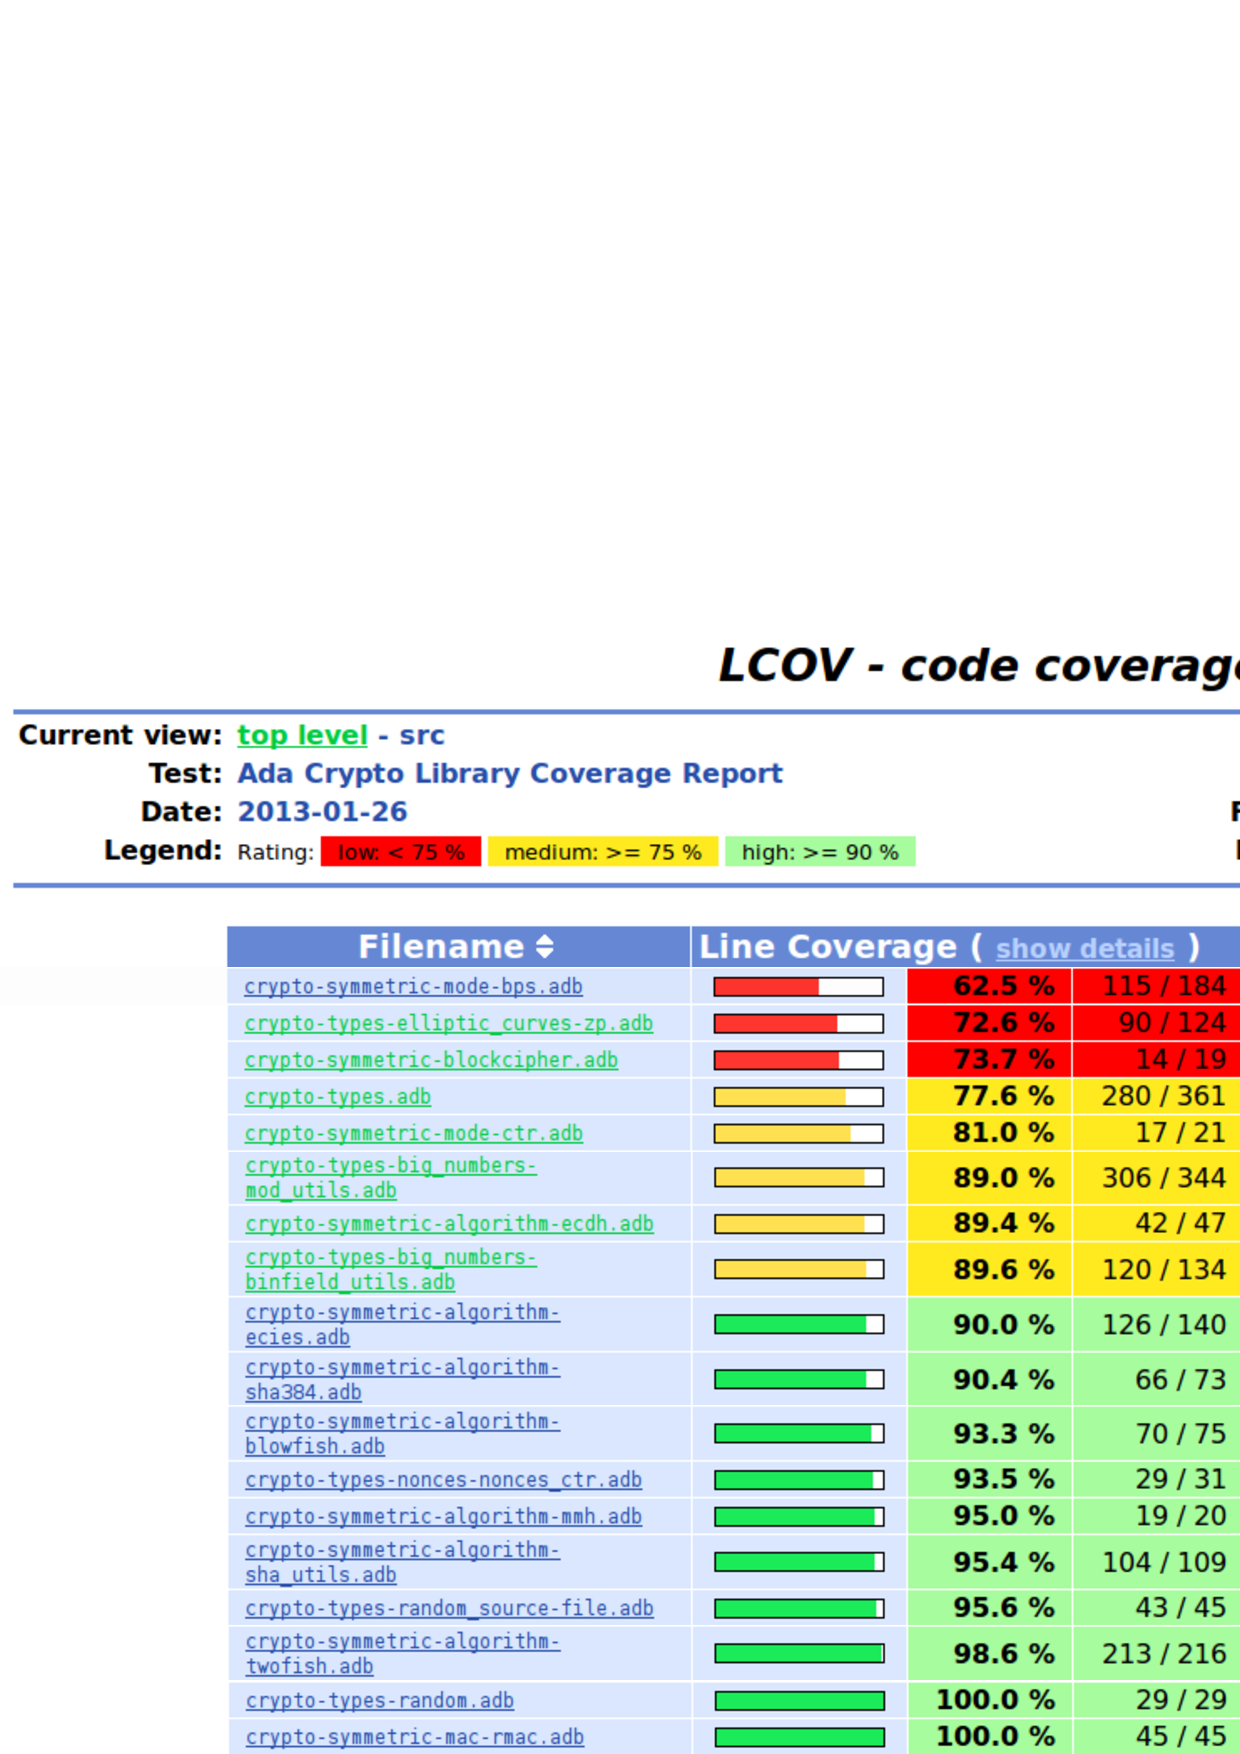
\includegraphics[scale=0.4]{Pictures/LCOV2.pdf} 
  \caption{The current test coverage of the ACL.}\label{LCOVS}
\end{figure}

\chapter{Regression Tests}
Figure \ref{ACLTEST} shows the layout of the test suites in the
ACL. To run the complete test, we need only run the file
\texttt{Test\_Tests}. Since the total test may last a few minutes, the
tests are additionally divided into five main categories:
\texttt{Test-Big\_Number}, \texttt{Test-Symmetric\_Ciphers},
\texttt{Test-Asymmetric\_Ciphers}, \texttt{Test-Hash} and
\texttt{Test-MISC}. All test cases for the big number library are in
\texttt{test\_suite\_big\_num1}, \texttt{test\_suite\_\-big\_num2},
\texttt{test\_suite\_big\_num3} and \texttt{test\_suite\_big\_num4},
the four suites are then collected in
\texttt{test\_suite\_big\_num\_all}.
\begin{figure}[h]
  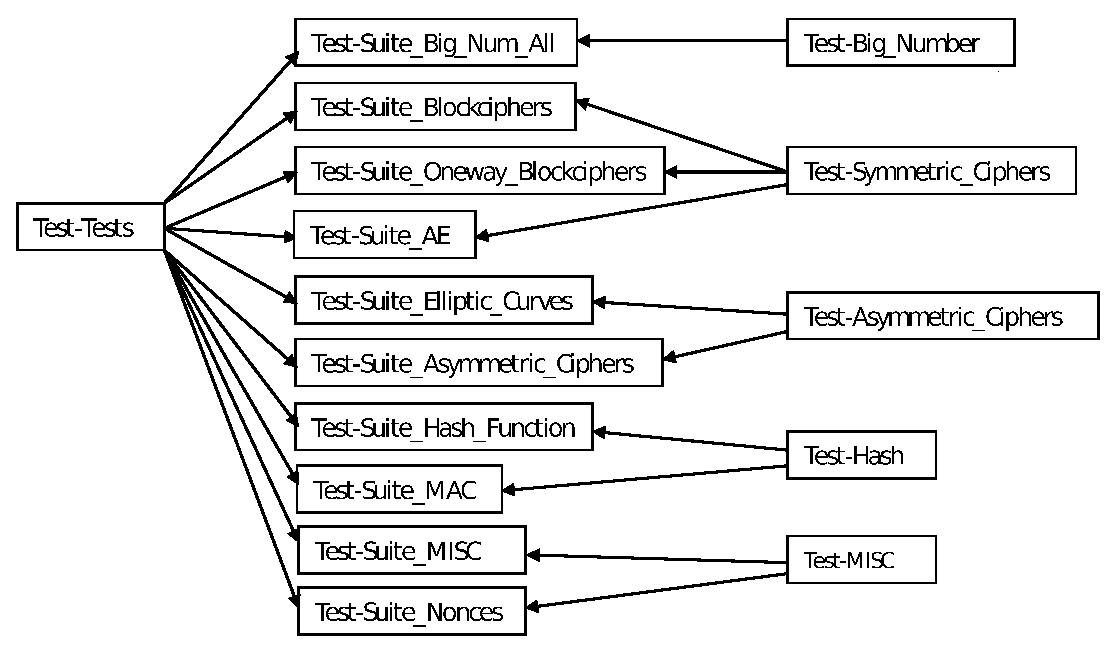
\includegraphics[scale=0.8]{./images/Layout_of_Test_Suite} 
  \caption{The structure of the ACL Test.}\label{ACLTEST}
\end{figure}

We start by writing a simple test case for the package
\texttt{Crypto.Types.Big\_Numbers}.
\begin{lstlisting}[numbers=left,caption={test-big\_number\_power.ads}\label{Big12}]
 with AUnit;
 with AUnit.Test_Cases;
 with Ada.Strings.Unbounded;  
 package Test.Big_Number_Power is
   use AUnit;
   use Ada.Strings.Unbounded;
   type Big_Number_Test is new Test_Cases.Test_Case with null record;
 
   procedure Register_Tests(T: in out Big_Number_Test);
   function Name(T: Big_Number_Test) return Test_String;
   procedure Big_Number_Test1(T: in out Test_Cases.Test_Case'Class);
 end Test.Big_Number_Power;
\end{lstlisting}

\begin{lstlisting}[numbers=left,caption={test-big\_number\_power.adb}\label{Big1}]
 with AUnit.Assertions; 
 with Crypto.Types.Big_Numbers;
 pragma Elaborate_All(Crypto.Types.Big_Numbers);
 package body Test.Big_Number_Power is
  package Big is new Crypto.Types.Big_Numbers(512);
  use Big;
  use Big.Utils;
  A: Big_Unsigned := To_Big_Unsigned("19");
  Result:Big_Unsigned:= To_Big_Unsigned("1978419655660313589123979");
	
  procedure Register_Tests(T : in out Big_Number_Test) is
	use Test_Cases.Registration;
  begin
	Register_Routine(T, Big_Number_Test1'Access,"Power");
  end Register_Tests;

  function Name(T : Big_Number_Test) return Test_String is
  begin
	return new String'("Big Number Tests");
  end Name;

  procedure Big_Number_Test1(T: in out Test_Cases.Test_Case'Class) is
    use AUnit.Assertions; 
  begin
    Assert(A ** A = Result, "Failed with A.");
  end Big_Number_Test1;
 end Test.Big_Number_Power;
\end{lstlisting}

Listing \ref{Big12} is the header file, which contains the definitions
of the types and operations required for the corresponding body
file. As shown in Listing \ref{Big1}, the function
\texttt{Register\_Tests()} (line 12) registsters the test case
\texttt{Big\_Number\_Test1}, and the function \texttt{Name()} (line
18) returns the name of the test case. The procedure
\texttt{Big\_Number\_Test1()} (line 23) contains the test case, which
tests if $19^{19}$ equals the result or not. The method
\texttt{Assert()} (line 26) checks the values, if the two values are
equal, then, the test is passed, else, the test case is failed with a
message "Failed with A." printed.

\begin{lstlisting}[numbers=left,caption={test-suite\_big\_number.ads}\label{BigS2}]
 with AUnit; use AUnit;
 with AUnit.Test_Suites;
 package Test.Suite_Big_Num is
   function Suite return Test_Suites.Access_Test_Suite;
 end Test.Suite_Big_Num;
\end{lstlisting}

\begin{lstlisting}[numbers=left,caption={test-suite\_big\_number.adb}\label{BigS}]
 with Test.Big_Number_Power;
 package body Test.Suite_Big_Num is
  Result	    : aliased Test_Suite;
  Test_Power : aliased Test.Big_Number_Power.Big_Number_Test;  
  function Suite return Access_Test_Suite is
  begin
    Add_Test(Result'Access, Test_Power'Access);    
    return Result'Access;
  end Suite;
 end Test.Suite_Big_Num;
\end{lstlisting}

Figure \ref{BigS2} is the header file of a test suite, and Figure
\ref{BigS} is the body file. As shown in Figure \ref{BigS}, the
function \texttt{Suite()} (line 5) gathers the test cases from the
file \texttt{Test.Big\_Number\_Power}.

\begin{lstlisting}[numbers=left,caption={test-big\_number.adb}\label{BigR}]
 with Test.Suite_Big_Num;
 with AUnit.Run;
 with AUnit.Reporter.Text;
 procedure Test.Big_Number is
   procedure Run is new AUnit.Run.Test_Runner_With_Results
   							(Test.Suite_Big_Num.Suite);
   Reporter : AUnit.Reporter.Text.Text_Reporter;
 begin
   Run(Reporter);
 end Test.Big_Number;
\end{lstlisting}

To run the tests, a runner (Figure \ref{BigR}) is created to provide a
routine that execute all the test cases in the suite. Test results are
reported using \texttt{Reporter}, which is specified when calling
\texttt{Run}. The final report is output once all test have been run,
so that they can be grouped (failed or passed).  We need only compile
the file \texttt{test-big\_Number.adb}.  Figure \ref{TEST} shows the
test result for the package \texttt{Crypto.Types.Big\_Numbers}.
\begin{figure}[h]
\centering
  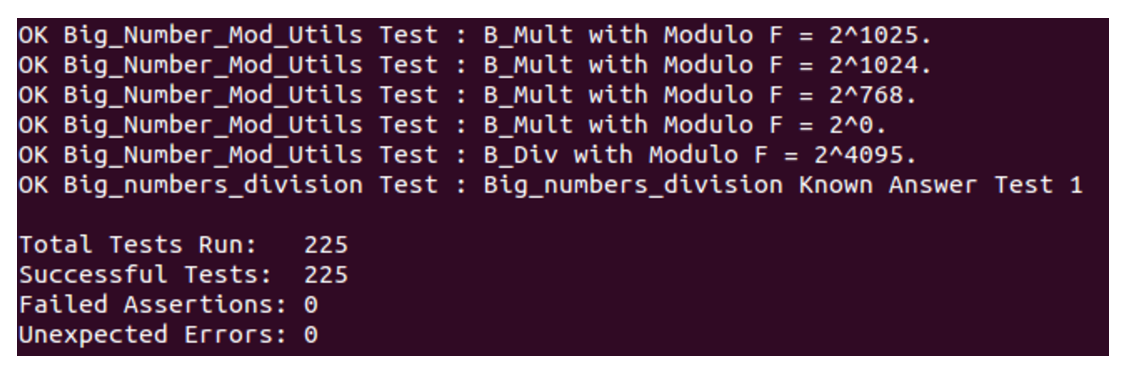
\includegraphics[scale=0.5]{./images/Big_Number}
  \caption{The result of a test.}\label{TEST}
\end{figure}

This is the same workflow when we do other tests. To run the whole
test cases, we need to compile the file \texttt{test-tests.adb}, it is
the runner, which collects all test suites for the ACL.

\bibliography{literature}
\end{document}